% Template for PLoS
%DIF LATEXDIFF DIFFERENCE FILE
%DIF DEL main_revised.tex   Mon May 21 13:34:56 2018
%DIF ADD main_final.tex     Sat Jun  2 11:24:45 2018
% Version 3.4 January 2017
%
% % % % % % % % % % % % % % % % % % % % % %
%
% -- IMPORTANT NOTE
%
% This template contains comments intended 
% to minimize problems and delays during our production 
% process. Please follow the template instructions
% whenever possible.
%
% % % % % % % % % % % % % % % % % % % % % % % 
%
% Once your paper is accepted for publication, 
% PLEASE REMOVE ALL TRACKED CHANGES in this file 
% and leave only the final text of your manuscript. 
% PLOS recommends the use of latexdiff to track changes during review, as this will help to maintain a clean tex file.
% Visit https://www.ctan.org/pkg/latexdiff?lang=en for info or contact us at latex@plos.org.
%
%
% There are no restrictions on package use within the LaTeX files except that 
% no packages listed in the template may be deleted.
%
% Please do not include colors or graphics in the text.
%
% The manuscript LaTeX source should be contained within a single file (do not use \input, \externaldocument, or similar commands).
%
% % % % % % % % % % % % % % % % % % % % % % %
%
% -- FIGURES AND TABLES
%
% Please include tables/figure captions directly after the paragraph where they are first cited in the text.
%
% DO NOT INCLUDE GRAPHICS IN YOUR MANUSCRIPT
% - Figs should be uploaded separately from your manuscript file. 
% - Figs generated using LaTeX should be extracted and removed from the PDF before submission. 
% - Figs containing multiple panels/subfigures must be combined into one image file before submission.
% For figure citations, please use "Fig" instead of "Figure".
% See http://journals.plos.org/plosone/s/figures for PLOS figure guidelines.
%
% Tables should be cell-based and may not contain:
% - spacing/line breaks within cells to alter layout or alignment
% - do not nest tabular environments (no tabular environments within tabular environments)
% - no graphics or colored text (cell background color/shading OK)
% See http://journals.plos.org/plosone/s/tables for table guidelines.
%
% For tables that exceed the width of the text column, use the adjustwidth environment as illustrated in the example table in text below.
%
% % % % % % % % % % % % % % % % % % % % % % % %
%
% -- EQUATIONS, MATH SYMBOLS, SUBSCRIPTS, AND SUPERSCRIPTS
%
% IMPORTANT
% Below are a few tips to help format your equations and other special characters according to our specifications. For more tips to help reduce the possibility of formatting errors during conversion, please see our LaTeX guidelines at http://journals.plos.org/plosone/s/latex
%
% For inline equations, please be sure to include all portions of an equation in the math environment.  For example, x$^2$ is incorrect; this should be formatted as $x^2$ (or $\mathrm{x}^2$ if the romanized font is desired).
%
% Do not include text that is not math in the math environment. For example, CO2 should be written as CO\textsubscript{2} instead of CO$_2$.
%
% Please add line breaks to long display equations when possible in order to fit size of the column. 
%
% For inline equations, please do not include punctuation (commas, etc) within the math environment unless this is part of the equation.
%
% When adding superscript or subscripts outside of brackets/braces, please group using {}.  For example, change "[U(D,E,\gamma)]^2" to "{[U(D,E,\gamma)]}^2". 
%
% Do not use \cal for caligraphic font.  Instead, use \mathcal{}
%
% % % % % % % % % % % % % % % % % % % % % % % % 
%
% Please contact latex@plos.org with any questions.
%
% % % % % % % % % % % % % % % % % % % % % % % %

\documentclass[10pt,letterpaper]{article}
\usepackage[top=0.85in,left=2.75in,footskip=0.75in]{geometry}

% % % % % % % % % % % % % % % % % % % % % % % %

%DIF 80c80
%DIF < % Extra symbols added
%DIF -------
% Extra symbols added (male and female) %DIF > 
%DIF -------
\usepackage{stix}
%DIF 82c82
%DIF < %Three part table - I think this is allowed
%DIF -------
%Three part table  %DIF > 
%DIF -------
\usepackage[flushleft]{threeparttable}

% % % % % % % % % % % % % % % % % % % % % % % %

% amsmath and amssymb packages, useful for mathematical formulas and symbols
\usepackage{amsmath}%amssymb

% Use adjustwidth environment to exceed column width (see example table in text)
\usepackage{changepage}

% Use Unicode characters when possible
\usepackage[utf8x]{inputenc}

% textcomp package and marvosym package for additional characters
\usepackage{textcomp,marvosym}

% cite package, to clean up citations in the main text. Do not remove.
\usepackage{cite}

% Use nameref to cite supporting information files (see Supporting Information section for more info)
\usepackage{nameref,hyperref}

% line numbers
\usepackage[right]{lineno}

% ligatures disabled
\usepackage{microtype}
\DisableLigatures[f]{encoding = *, family = * }

% color can be used to apply background shading to table cells only
\usepackage[table]{xcolor}

% array package and thick rules for tables
\usepackage{array}

% create "+" rule type for thick vertical lines
\newcolumntype{+}{!{\vrule width 2pt}}

% create \thickcline for thick horizontal lines of variable length
\newlength\savedwidth
\newcommand\thickcline[1]{%
  \noalign{\global\savedwidth\arrayrulewidth\global\arrayrulewidth 2pt}%
  \cline{#1}%
  \noalign{\vskip\arrayrulewidth}%
  \noalign{\global\arrayrulewidth\savedwidth}%
}

% \thickhline command for thick horizontal lines that span the table
\newcommand\thickhline{\noalign{\global\savedwidth\arrayrulewidth\global\arrayrulewidth 2pt}%
\hline
\noalign{\global\arrayrulewidth\savedwidth}}


% Remove comment for double spacing
%\usepackage{setspace} 
%\doublespacing

% Text layout
\raggedright
\setlength{\parindent}{0.5cm}
\textwidth 5.25in 
\textheight 8.75in

% Bold the 'Fig #' in the caption and separate it from the title/caption with a period
% Captions will be left justified
\usepackage[aboveskip=1pt,labelfont=bf,labelsep=period,justification=raggedright,singlelinecheck=off]{caption}
\renewcommand{\figurename}{Fig}

% Use the PLoS provided BiBTeX style
\bibliographystyle{plos2015}

% Remove brackets from numbering in List of References
\makeatletter
\renewcommand{\@biblabel}[1]{\quad#1.}
\makeatother

% Leave date blank
\date{}

% Header and Footer with logo
\usepackage{lastpage,fancyhdr,graphicx}
\usepackage[outdir=./]{epstopdf}
\pagestyle{myheadings}
\pagestyle{fancy}
\fancyhf{}
\setlength{\headheight}{27.023pt}
\lhead{
\includegraphics[width=2.0in]{PLOS-submission.eps}}
\rfoot{\thepage/\pageref{LastPage}}
\renewcommand{\footrule}{\hrule height 2pt \vspace{2mm}}
\fancyheadoffset[L]{2.25in}
\fancyfootoffset[L]{2.25in}
\lfoot{\sf PLOS}
%% Include all macros below

%for figure alignment
\usepackage[export]{adjustbox}

\newcommand{\lorem}{{\bf LOREM}}
\newcommand{\ipsum}{{\bf IPSUM}}


%reference equations in appendices
\usepackage{xr}
\externaldocument{S1Appendix_revised}
\externaldocument{S2Appendix_revised}
\externaldocument{S3Appendix_revised}

%for figures
%\usepackage{epstopdf}


%% END MACROS SECTION
%DIF PREAMBLE EXTENSION ADDED BY LATEXDIFF
%DIF UNDERLINE PREAMBLE %DIF PREAMBLE
\RequirePackage[normalem]{ulem} %DIF PREAMBLE
\RequirePackage{color}\definecolor{RED}{rgb}{1,0,0}\definecolor{BLUE}{rgb}{0,0,1} %DIF PREAMBLE
\providecommand{\DIFadd}[1]{{\protect\color{blue}\uwave{#1}}} %DIF PREAMBLE
\providecommand{\DIFdel}[1]{{\protect\color{red}\sout{#1}}}                      %DIF PREAMBLE
%DIF SAFE PREAMBLE %DIF PREAMBLE
\providecommand{\DIFaddbegin}{} %DIF PREAMBLE
\providecommand{\DIFaddend}{} %DIF PREAMBLE
\providecommand{\DIFdelbegin}{} %DIF PREAMBLE
\providecommand{\DIFdelend}{} %DIF PREAMBLE
%DIF FLOATSAFE PREAMBLE %DIF PREAMBLE
\providecommand{\DIFaddFL}[1]{\DIFadd{#1}} %DIF PREAMBLE
\providecommand{\DIFdelFL}[1]{\DIFdel{#1}} %DIF PREAMBLE
\providecommand{\DIFaddbeginFL}{} %DIF PREAMBLE
\providecommand{\DIFaddendFL}{} %DIF PREAMBLE
\providecommand{\DIFdelbeginFL}{} %DIF PREAMBLE
\providecommand{\DIFdelendFL}{} %DIF PREAMBLE
%DIF END PREAMBLE EXTENSION ADDED BY LATEXDIFF

\begin{document}
\vspace*{0.2in}

% Title must be 250 characters or less.
\begin{flushleft}
{\Large
\textbf\newline{Haploid selection, sex-ratio bias, and transitions between sex-determining systems} % Please use "sentence case" for title and headings (capitalize only the first word in a title (or heading), the first word in a subtitle (or subheading), and any proper nouns).
}
\newline
% Insert author names, affiliations and corresponding author email (do not include titles, positions, or degrees).
\\
Michael Francis Scott\textsuperscript{1\Yinyang*},
Matthew Miles Osmond\textsuperscript{2\Yinyang},
Sarah Perin Otto\textsuperscript{2}
\\
\bigskip
\textbf{1} UCL Genetics Institute, Department of Genetics, Evolution and Environment, University College London, Gower Street, London WC1E 6BT 
\\
\textbf{2} Department of Zoology, University of British Columbia, \#4200 - 6270 University Boulevard, Vancouver, BC, Canada V6T 1Z4
\\
\bigskip

% Insert additional author notes using the symbols described below. Insert symbol callouts after author names as necessary.
% 
% Remove or comment out the author notes below if they aren't used.
%
% Primary Equal Contribution Note
\Yinyang These authors contributed equally to this work.

% Additional Equal Contribution Note
% Also use this double-dagger symbol for special authorship notes, such as senior authorship.
%\ddag These authors also contributed equally to this work.

% Current address notes
%\textcurrency Current Address: Dept/Program/Center, Institution Name, City, State, Country % change symbol to "\textcurrency a" if more than one current address note
% \textcurrency b Insert second current address 
% \textcurrency c Insert third current address

% Deceased author note
%\dag Deceased

% Group/Consortium Author Note
%\textpilcrow Membership list can be found in the Acknowledgments section.

% Use the asterisk to denote corresponding authorship and provide email address in note below.
* m.f.scott@ucl.ac.uk

\end{flushleft}
% Please keep the abstract below 300 words
%DIF < currently 308 words
%DIF > %%%%%%%%%%%%%%%%%%%%%%%%%
\section*{Abstract}
%DIF > %%%%%%%%%%%%%%%%%%%%%%%%%
Sex determination is remarkably dynamic; many taxa display shifts in the location of sex-determining loci or the evolution of entirely new sex-determining systems. 
Predominant theories for why we observe such transitions generally conclude that novel sex-determining systems are favoured by selection if they equalise the sex ratio or increase linkage with a locus that experiences different selection in males vs.\ females. 
We use population genetic models to extend these theories in two ways: 
(1) We consider the dynamics of loci very tightly linked to the ancestral sex-determining loci, e.g., within the non-recombining region of the ancestral sex chromosomes. 
Variation at such loci can favour the spread of new sex-determining systems in which the heterogametic sex changes (XY to ZW or ZW to XY) and the new sex-determining region is less closely linked (or even unlinked) to the locus under selection. 
%DIF < , which is \textcolor{red}{not expected from previous theory}. 
(2) We consider selection upon haploid genotypes either during gametic competition (e.g., pollen competition) or meiosis (i.e., non-Mendelian segregation), which can cause the zygotic sex ratio to become biased. 
Haploid selection can drive transitions between sex-determining systems without requiring selection to act differently in diploid males vs.\ females. 
With haploid selection, we find that transitions between male and female heterogamety can evolve where linkage with the sex-determining locus is either strengthened or weakened. 
%DIF < Furthermore, we find that the selective strengths exerted by the sex-ratio and associations with selected alleles are often equivalent. 
Furthermore, we find that sex-ratio biases may increase or decrease with the spread of new sex chromosomes, which implies that transitions between sex-determining systems cannot be simply predicted by selection to equalise the sex ratio.
In fact, under many conditions, we find that transitions in sex determination are favoured equally strongly in cases where the sex ratio bias increases or decreases.
%DIF < Furthermore, we find that the selective forces to equalize the sex ratio are equally important to selective forces that generate skewed sex ratios when accounting for the spread of new sex chromosomes.
%DIF < This allows sex-ratio biases to increase or decrease with the spread of new sex chromosomes and implies that transitions between sex-determining systems cannot be simply predicted by selection to equalise the sex ratio. 
Overall, our models predict that sex determination systems should be highly dynamic, particularly when haploid selection is present, consistent with the evolutionary lability of this trait in many taxa.
%DIF < Overall, our models reveal that transitions between sex-determining systems, particularly transitions where the heterogametic sex changes, can be driven by loci in previously unpredicted genomic locations that experience selection during diploid and/or haploid phases.
%DIF < Our results predict conditions under which sex-determining systems are likely to be labile and draw connections with sex-ratio evolution.


% Please keep the Author Summary between 150 and 200 words
% Use first person. PLOS ONE authors please skip this step. 
% Author Summary not valid for PLOS ONE submissions.   
%DIF < currently 193 words
%DIF > %%%%%%%%%%%%%%%%%%%%%%%%%
\section*{Author summary}
%DIF > %%%%%%%%%%%%%%%%%%%%%%%%%
Systems of sex determination are strikingly diverse and labile in many clades. 
This poses the question: what drives transitions between sex-determining systems? 
Here, we use models to derive conditions under which new sex-determining systems spread. 
Prevailing views suggest that new sex-determining systems are favoured when they equalize the sex ratio and/or when they are more closely linked to genes that experience differential selection in males and females. 
Our models include selection upon haploid genotypes (meiotic drive or gametic competition), which biases the sex-ratio and occurs differently in male and female gametes. 
Surprisingly, we find the two forces (selection to equalize the sex ratio and the benefits of hitchhiking alongside driven alleles that distort the sex ratio) will often be equally strong, and thus neither is sufficient to explain the spread of new sex-determining systems in every case. 
We also find that new sex-determining alleles can spread despite being less closely linked to selected loci as long as initial linkage is tight or haploid selection is present.
Our models therefore predict that loci in previously unexpected genomic locations and/or experiencing various types of selection (including haploid selection) can now be implicated as drivers of transitions between sex-determining systems. 

\linenumbers

% Use "Eq" instead of "Equation" for equation citations.
%DIF > %%%%%%%%%%%%%%%%%%%%%%%%%
\section*{Introduction}
%DIF < TRANSITIONS ARE COMMON
%DIF > %%%%%%%%%%%%%%%%%%%%%%%%%
Animals and angiosperms exhibit extremely diverse sex-determining systems (reviewed in~\cite{Bull:1983vi,Charlesworth:2010it,Beukeboom:2014vb,Bachtrog:2014bx, Pennell2018}). 
Among species with genetic sex determination (GSD), some taxa have heterogametic males (XY) and homogametic females (XX), including %DIF < non-monotreme? I think monotremes have XY but tonnes of translocations, giving: X1,X2...X6 Y1
mammals and most dioecious plants~\cite{Ming:2011iy}; whereas other taxa have homogametic males (ZZ) and heterogametic females (ZW), including Lepidoptera and birds. 
Within several taxa, the chromosome that harbours the master sex-determining locus changes, due either to translocation of the master sex-determining locus or to the evolution of a new master locus.  
During these transitions, the heterogametic sex can remain the same (hereafter `cis-GSD transitions') as in Salmonids~\cite{Li:2011fm,Yano:2012di}, Diptera~\cite{Vicoso:2015hf}, and \textit{Oryzias}~\cite{Myosho:2012fv}. 
%DIF < Presentation at evolution found neo sex chromosome in birds, doesn't seem to be published or bioRxiv yet (consider pers com.), title: A previously unknown neo-sex chromosome mediates plumage divergence and speciation in hybridizing birds Jason Sardell; Elizabeth Cooper; J. Albert C. Uy. I wonder if this is actually a fusion event though?
Alternatively, species can switch between male and female heterogamety (XY$\leftrightarrow$ZW, hereafter `trans-GSD transitions'), as in snakes~\cite{Gamble2017}, lizards~\cite{Ezaz:2009tk}, eight of 26 teleost fish families~\cite{Mank:2006bt}, true fruit flies (Tephritids,~\cite{Vicoso:2015hf}), amphibians~\cite{Hillis:1990gu}, the angiosperm genus \textit{Silene}~\cite{Slancarova:2013dq}, the angiosperm family \textit{Salicaceae}~\cite{Pucholt2015,Pucholt2017} and Coleoptera and Hemiptera (plate 2~\cite{Beukeboom:2014vb}).
Indeed, in some cases, both male and female heterogametic sex-determining systems can be found in the same species, as reported in houseflies~\cite{Macdonald1978}, midges~\cite{Thompson1971}, frogs~\cite{Ogata:2007jm}, cichlid fish~\cite{Ser:2010iq}, tilapia~\cite{Lee2004}, sea bass~\cite{Vandeputte2007}, and lab-strains of Zebrafish~\cite{Liew2012,Wilson2014}.
In addition, multiple transitions have occurred between genetic and environmental sex-determining systems (GSD$\leftrightarrow$ESD), e.g., in reptiles and fishes~\cite{Conover:1987in,Mank:2006bt,Pokorna:2009ui,Ezaz:2009tk,Pen:2010kk,Holleley:2015hc, Pennell2018}.
In sum, accumulating evidence indicates that transitions between sex-determining systems are common~\cite{Bachtrog:2014bx}.

%DIF < MAJOR MECHANISMS
%DIF < (1) sex-ratio selection
%DIF < Predominant theories accounting for transitions between GSD systems by selection involve sex-ratio selection or selective differences between the sexes (e.g., sexually antagonistic selection)~\cite{Blaser2012, Beukeboom:2014vb,vanDoorn2014re}. 
%DIF < \citet{Bull:1977wt} shows that direct selection on new sex determination loci can allow them to spread and switch between male and female heterogamety. 
It has been suggested that sex-ratio selection is a particularly dominant force in the evolution of sex determination (e.g., Bull, 1983, p 66-67 ~\cite{Bull:1983vi}; Buekeboom and Perrin, 2014, Chapter 7~\cite{Beukeboom:2014vb}). 
Classic `Fisherian' sex-ratio selection favours a 1:1 zygotic sex ratio when assuming that males and females are equally costly to produce~\cite{Fisher:1930wy,Charnov:1982wg}. 
This follows from the fact that, for an autosomal locus, half of the genetic material is inherited from a male and half from a female~\cite{West:2009we}. 
Thus, if the sex ratio is biased, an individual of the rarer sex will, on average, contribute more genetic material to the next generation. 
Selection therefore typically favours mutants that increase investment in the rarer sex, including new sex determination systems.
%DIF < Because the sex ratio is directly determined by the sex-determining system, it has been suggested that sex-ratio selection is a particularly dominant force in the evolution of sex determination (e.g., Bull, 1983, p 66-67 ~\cite{Bull:1983vi}; Buekeboom and Perrin, 2014, Chapter 7~\cite{Beukeboom:2014vb}). 

%DIF < MAJOR MECHANISMS
%DIF < (2) sex-antagonism
The evolution of sex determination is also thought to be strongly influenced by differences in selection between the sexes ~\cite{Blaser2012, Beukeboom:2014vb,vanDoorn2014re}.
For example, loci experiencing sexual antagonism have been shown to favour the spread of new genetic sex-determining alleles that are closely linked~\cite{vanDoorn:2007eu,vanDoorn:2010hu,Muralidhar2018}. 
%DIF < van Doorn and Kirkpatrick~\cite{vanDoorn:2007eu,vanDoorn:2010hu} and Muralidhar and Veller~\cite{Muralidhar2018} have shown that new sex-determining alleles can be favoured if they arise at loci in close linkage with a locus that experiences sexual antagonism. 
Linkage allows a stronger favourable association to build up between a male-beneficial allele and a neo-Y allele, for example. 
Such associations can favour cis-GSD transitions~\cite{vanDoorn:2007eu}, trans-GSD transitions~\cite{vanDoorn:2010hu}, and new partially-masculinizing or partially-feminizing alleles in a population with ESD~\cite{Muralidhar2018}.
%DIF < However, any sexually-antagonistic loci that are more closely linked to the ancestral sex-determining locus should develop similar, favourable associations and are expected to hinder the spread of a new sex-determining system~\cite{vanDoorn:2007eu,vanDoorn:2010hu}. 
By similar logic, however, existing sexually-antagonistic alleles associated with the current sex-determining locus are expected to hinder the spread of a new sex-determining system~\cite{vanDoorn:2007eu,vanDoorn:2010hu}.

%DIF < Tight linkage Model Feature and Result
One novel feature of the models developed here is that we explicitly consider the maintenance of genetic variation around the ancestral sex-determining locus (e.g., within the non-recombining region of a sex chromosome).  
%DIF < during trans-GSD transitions
%DIF < , when considering loci in very tight linkage with the ancestral sex-determining locus (e.g., within the non-recombining region of a sex chromosome), 
%DIF < \textcolor{red}{[vDK2007 does "explicitly" consider this as well (although on pg 15 of their SOM they say they will ignore equilibrium A, as it is stable under a "limited range of biologically relevant parameter combinations"; perhaps haploid selection changes this impression), but only for cis-GSD transitions. They find that if equil B is stable the neo-Y never spreads when r=0. vDK2010 does not "explicitly" calculate pX and pY, which are required to see if their equation 7 is positive or negative, but nowhere do they seem to say that weaker linkage \textit{can't} evolve given r initially small.]}
%DIF < we explicitly calculate ancestral polymorphisms. 
%DIF < Our analysis reveals that, under various forms of selection, the ancestral-X can carry suboptimal alleles for females and/or the ancestral-Y can carry female-beneficial alleles. 
Counterintuitively, when linkage is tight between the sex-determining locus and a selected locus, an allele good for females can be at higher frequency on the ancestral-Y than on the ancestral-X under a variety of forms of selection.
In addition, selection on ancestral-X chromosomes in males can prevent the X from becoming optimally specialised for female-beneficial alleles. 
These factors, in turn, can favour a new ZW sex-determining locus that has weaker linkage with loci under selection, which was not revealed by previous theory \cite{vanDoorn:2010hu}. A similar argument applies to ZW$\rightarrow$XY transitions. 
Thus, we show that selected loci in very tight linkage with the ancestral GSD locus can favour trans-GSD transitions during which linkage associations are actually weakened. 

%DIF < Haploid selection model feature and discussion of why needed
Most significantly, we include haploid selection (gametic competition or meiotic drive) in models describing cis-GSD, trans-GSD, and GSD to ESD transitions.
This poses an apparent evolutionary problem. 
On one hand, haploid selection is typically sex-limited in that it usually occurs among gametes produced by one sex only~\cite{Mulcahy:1996ha,JOSEPH:2004haa,Ubeda:2005gw,Lindholm:2016cw}. 
Therefore, one might expect new sex-determining systems to benefit from close linkage with haploid selected loci, as found for loci that experience diploid-sex-differences in selection~\cite{vanDoorn:2007eu,vanDoorn:2010hu, Muralidhar2018}. 
On the other hand, associations between sex-determining loci and haploid selected loci generate biased zygotic sex ratios, which should generally hinder the spread of new sex-determining systems. 

%DIF < Previous models with haploid selection
Two previous studies have considered the spread of GSD with sex-limited meiotic drive~\cite{Kozielska:2010vm,Ubeda:2015fx} under a limited number of possible genetic architectures and diploid selective regimes. 
Ubeda et al. (2015)~\cite{Ubeda:2015fx} considered ancestral-ESD (with no sex-ratio bias) and numerically showed that new GSD alleles can spread if they arise in linkage with meiotic drive loci. 
For example, a masculinizing allele spreads in association with an allele that is favoured during male meiosis, causing sex ratios to become male-biased.
This suggests that the benefits of associating with driving alleles can overwhelm selection to balance the sex ratio.
%DIF < , at least when new sex-determining alleles are rare. 
However, Kozielska et al. (2010)~\cite{Kozielska:2010vm} considered an ancestral GSD system that is perfectly linked to a meiotic driver and therefore exhibiting an ancestral sex ratio bias. 
They found that a new, completely unlinked, GSD system can spread if it generates the rarer sex, creating a balanced sex ratio. 
This suggests that Fisherian sex-ratio selection can overwhelm the benefits of being associated with driving alleles. 
It is thus currently unclear when haploid selection favors increased versus decreased linkage between haploid selected loci and a new sex-determining locus. 
In addition, because the sex ratio is determined by linkage between haploid selected loci and the sex-determining locus, it is also unclear when Fisherian sex-ratio selection is the most important driver of transitions between sex-determining systems. 

%DIF < main results
Here, we analytically find the conditions under which new GSD or ESD systems spread in ancestral GSD systems with any degree of linkage between the loci involved and arbitrary forms of haploid and diploid selection. 
Doing so, we reconcile and generalize the results of Kozielska et al. (2010)~\cite{Kozielska:2010vm} and Ubeda et al. (2015)~\cite{Ubeda:2015fx} by deriving conditions for the spread of new GSD systems that alter linkage with haploid selected loci.
Our result is qualitatively distinct from those for diploid selection alone~\cite{vanDoorn:2007eu,vanDoorn:2010hu} and suggests that haploid selection is more likely to promote transitions between sex-determination systems. 
We also show that transitions involving haploid selection cannot be simply explained by invoking sex-ratio selection. 
In particular, under a wide range of conditions, we show that transitions in sex-determining system are favoured \textit{equally strongly} in situations where sex-ratio biases increase or decrease (and in situations where sex-ratio biases are ancestrally present or absent). 
Finally, we show that ESD may not evolve, even if the sex ratio is initially biased by haploid selection, which is not predicted by previous theories for transitions to ESD~\cite{Charnov:1982wg,Bull:1983vi,West:2009we}. 
%DIF < Together, our results suggest that neither selection to equalize the sex ratio nor the benefits of associating with haploid selected alleles is an overwhelming force driving transitions between sex-determining systems. 
Together, our results suggest that both selection to equalize the sex ratio and the benefits of associating with haploid selected alleles can drive transitions between sex-determining systems, leading to stronger or weaker sex-linkage and increased or decreased sex ratio bias. 

%DIF < Here we use mathematical models to find the conditions under which new sex-determining systems spread when individuals experience selection at both diploid and haploid stages, which allows fitness differences between the sexes and sex ratio biases to occur simultaneously
\DIFdelbegin %DIFDELCMD < 

%DIFDELCMD < %%%
%DIF < Haploid selection results
%DIFDELCMD < 

%DIFDELCMD < %%%
%DIF < The sex ratio is directly determined by the sex-determining system, and it has therefore been suggested that sex-ratio selection is a dominant force in the evolution of sex determination (e.g., Bull, 1983, p 66-67 ~\cite{Bull:1983vi}; Buekeboom and Perrin, 2014, Chapter 7~\cite{Beukeboom:2014vb}). 
%DIF < `Fisherian' sex-ratio selection favours a 1:1 zygotic sex ratio when assuming that males and females are equally costly to produce~\cite{Fisher:1930wy,Charnov:1982wg}.
%DIF < This follows from the fact that, for an autosomal locus, half of the genetic material is inherited from a male and half from a female~\cite{West:2009we}. 
%DIF < Thus, if the sex ratio is biased, an individual of the rarer sex will, on average, contribute more genetic material to the next generation. 
%DIF < Selection therefore favours mutants that increase investment in the rarer sex.
%DIFDELCMD < 

%DIFDELCMD < %%%
%DIF < The default mode of sex-ratio selection is `Fisherian' sex-ratio selection, which favours equal investment in male and female offspring \citep[i.e., a 1:1 zygotic sex ratio when assuming that males and females are equally costly to produce,][]{Fisher:1930wy,Charnov:1982wg}. 
%DIF < Given that the sex-determining system can directly affect the sex ratio, we might expect Fisherian sex-ratio selection to influence the spread of new sex-determining systems. 
%DIF < In the case of sex-chromosome evolution, Kozielska et al. (2010)~\cite{Kozielska:2010vm} consider systems in which the ancestral sex chromosomes experience meiotic drive (e.g., where driving X or Y chromosomes are inherited disproportionately often), which causes sex ratios to become biased~\cite{Hamilton:1967ts}. 
%DIF < They find that masculinizing or feminizing mutations that arise at a new, unlinked locus (i.e., neo-Y or neo-W chromosomes) can then spread, which restore an even sex ratio. 
%DIF < However, starting from ESD, Ubeda et al. (2015)~\cite{Ubeda:2015fx} have numerically shown that sex-specific meiotic drive can allow masculinizing and feminizing mutations to spread (i.e., ESD $\rightarrow$ GSD) despite causing a sex-ratio bias.
%DIFDELCMD < 

%DIFDELCMD < %%%
%DIF < HOLES IN CURRENT THEORY
%DIF < (1) haploid selection; it exists in many spp
%DIF < While both opposing selection in the diploid sexes and sex-ratio selection surely influence the evolution of new sex-determining factors, so too might selection in the haploid phase.
%DIFDELCMD < 

%DIFDELCMD < %%%
%DIF < HOLES IN CURRENT THEORY
%DIF < (2) haploid selection; it can complicate outcomes for SD transitions
%DIF < There are various ways by which haploid selection could influence transitions between sex-determining systems. 
%DIF < If we assume that haploid selection at any particular locus predominantly occurs in one sex (e.g., meiotic drive during spermatogenesis), then such loci experience a form of sex-specific selection. 
%DIF < In this respect, we might expect that haploid selection would affect transitions between sex-determining systems in a similar manner to sex-specific diploid selection (as explored in~\cite{vanDoorn:2007eu,vanDoorn:2010hu}). 
%DIF < That is, new masculinizing mutations (neo-Y alleles) could be favoured via associations with alleles that are beneficial in the male haploid stage (e.g., \cite{Ubeda:2015fx}). 
%DIF < Kozielska et al. (2010)~\cite{Kozielska:2010vm} have shown this to be theoretically possible for the special case of perfect linkage between the new sex-determining locus and a locus that experiences meiotic drive in one sex, under a limited number of forms of diploid selection.
%DIF < Similarly, Ubeda et al. (2015)~\cite{Ubeda:2015fx} numerically show that sex-specific meiotic drive can allow masculinizing and feminizing mutations to spread in an ancestrally environmental-sex-determination system, again under a limited number of forms of diploid selection. 
%DIF < On the other hand, sex ratios can also become biased by linkage between the sex-determining locus and a locus that harbours genetic variation in haploid fitness, as indeed occurs in the two examples above.
%DIF < There are also several known empirical cases of sex-ratio bias caused by sex-linked meiotic drive alleles (Burt and Trivers, 2006, Chapter 6~\cite{Burt:2006}) or selection among X- and Y-bearing pollen~\cite{Lloyd:1974tz,Conn:1981uw,Stehlik:2005ul,Stehlik:2006to,Field:2012fd,Field:2013cc}. 
%DIF < Sex-ratio selection can thus select against the spread of linked sex-determining alleles and favour the invasion of alternative, unlinked sex-determination systems \cite{Kozielska:2010vm,Ubeda:2015fx}.
%DIF < It is not yet clear when new sex-determining alleles are favoured by associations with haploid selected alleles vs. sex-ratio bias, especially under a wide range of possible diploid selection regimes (e.g., sex-antagonism, overdominance).	
%DIFDELCMD < 

%DIFDELCMD < %%%
%DIF < We consider both selected loci that are loosely linked to the sex-determining region (e.g., on an autosome) and selected loci that are in very tight linkage with the ancestral sex-determining locus (e.g., within the non-recombining sex-determining region).
%DIF < Our main findings are three:
%DIF < (1) transitions between sex-determining systems can decrease or increase sex-ratio bias, and with sufficiently loose linkage between the selected locus and the sex-determining locus, the selective force exerted by sex-ratio selection and favourable associations with haploid-selected alleles are exactly equivalent;
%DIF < (2) ancestrally-tight sex-linkage and haploid selection allow trans-GSD transitions that weaken sex-linkage; and
%DIF < (3) haploid selection removes the need for sex-antagonism, increasing the range of scenarios that select for transitions between sex-determining systems.
%DIFDELCMD < 

%DIFDELCMD < %%%
%DIF < MAIN FINDINGS IN GENERAL TERMS
%DIF < We find that the spread of novel sex-determining systems is influenced by both Fisherian sex-ratio selection and by selection on linked alleles. 
%DIF < We find that sex-ratio biases caused by haploid selection can exert Fisherian sex-ratio selection upon novel sex-determiners but that their spread is also determined by selection on genetically-associated alleles. 
%DIF < Indeed, it is only when haploid-selected loci are tightly linked to the ancestral sex-determining region (and so sex-ratio biases are initially large) that we see an asymmetry between selection for XY to ZW transitions and ZW to XY transitions (e.g., because haploid selection in males only causes biased zygotic sex ratios in an ancestrally XY system).
%DIF < Fisherian sex-ratio selection does not always dominate; it is possible for selection on linked alleles to drive turnover between sex-determining systems despite causing increasingly biased sex ratios, and our analytical results elucidate what is required for this to be so.
%DIF < Because sex-determining loci are often found within a region of suppressed recombination, there can be a significant number of tightly linked loci. 
%DIF < We find that loci tightly linked with the sex-determining locus can drive transitions in which the heterogametic sex changes, even when the new sex-determining locus is less closely linked to loci under selection (either including haploid selection or not). 
%DIFDELCMD < 

%DIFDELCMD < %%%
\DIFdelend %DIF > %%%%%%%%%%%%%%%%%%%%%%%%%
\section*{Model}
%DIF > %%%%%%%%%%%%%%%%%%%%%%%%%

%DIF < genetic system
We consider transitions between ancestral and novel sex-determining systems using a three-locus model, each locus having two alleles (Fig \ref{fig:model_outline}). A full description of our model, including recursion equations, is given in \nameref{app:recurs}. 
Locus $\mathbf{X}$ is the ancestral sex-determining region, with alleles X and Y (or Z and W).
Locus $\mathbf{A}$ is a locus under selection, with alleles $A$ and $a$.
Locus $\mathbf{M}$ is a novel sex-determining region, at which the null allele ($M$) is initially fixed in the population such that sex of zygotes is determined by the genotype at the ancestral sex-determining region, $\mathbf{X}$; XX genotypes become females and XY become males (or ZW become females and ZZ become males). 
To evaluate the evolution of new sex-determining systems, we consider the spread of a novel sex-determining allele ($m$) at the $\mathbf{M}$ locus. 
%DIF < We only do invasion analytically though (is this sentence still ok?)

Here, we assume that the $\mathbf{M}$ locus is `epistatically dominant' over the $\mathbf{X}$ locus such that zygotes with at least one $m$ allele develop as females with probability $k$ and as males with probability $1-k$, regardless of the $\mathbf{X}$ locus genotype. 
With $k=0$, the $m$ allele is a masculinizer (a neo-Y allele) and with $k=1$ the $m$ allele is a feminizer (a neo-W allele). 
With intermediate $k$, we can interpret $m$ as an environmental sex-determination (ESD) allele, such that zygotes develop as females in a proportion ($k$) of the environments they experience. 
The assumption that derived sex-determining loci are epistatically dominant is motivated by empirical systems in which multiple sex determining alleles segregate (i.e., X, Y, Z, and W alleles present), such as, cichlid fish~\cite{Ser:2010iq}, platyfish (\textit{Xiphophorus maculatus}~\cite{Kallman1968}), houseflies (\textit{Musca domestica}~\cite{Dubendorfer2002}), western clawed frogs (\textit{Xenopus tropicalis}~\cite{Roco2015}) and \textit{Rana rugosa}~\cite{Ogata:2007jm}.  
Nevertheless, our supplementary analysis file (\nameref{file:Mathematica}) allows other dominance relationships between loci to be specified (see also \cite{vanDoorn:2007eu} supplementary material for a numerical analysis). 
%DIF < See also the supplementary material in \cite{vanDoorn:2007eu} for a numerical analysis that relaxes the assumption of epistatic dominance.
%DIF < We also analyze a model of maternally-controlled environmental sex-determination, where mothers with at least one $m$ allele produce daughters with probability $k$. 

%DIF < %%%%%%%%%%%%%%%%%%%%%%%%%%%%%%%%%%%%%%%%%%%%%%%%%%%%%%%%
%DIF < Model Outline
%DIF < %%%%%%%%%%%%%%%%%%%%%%%%%%%%%%%%%%%%%%%%%%%%%%%%%%%%%%%%
\begin{figure}[!h]
%\centering
\DIFdelbeginFL %DIFDELCMD < \centerline{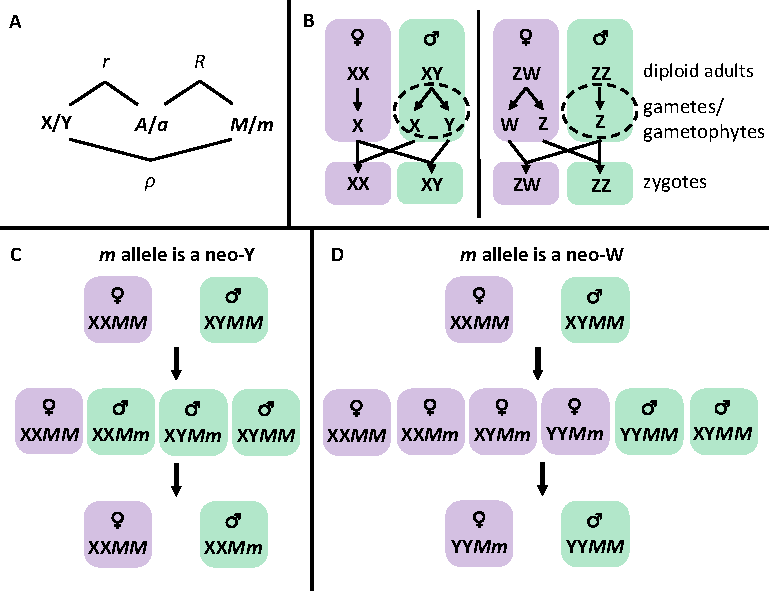
\includegraphics[width=0.9\linewidth]{../Plots/Sex_determination_outline.pdf}}
%DIFDELCMD < %%%
\DIFdelendFL %DIF > \centerline{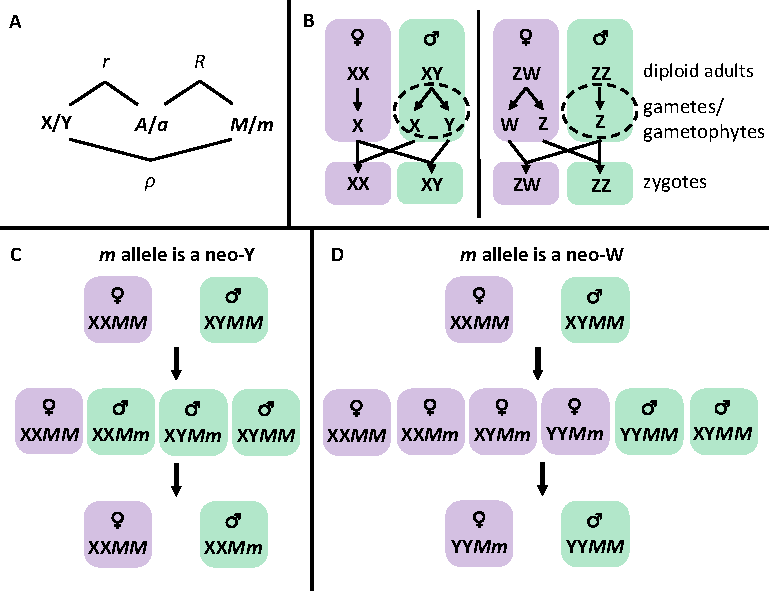
\includegraphics[width=0.9\linewidth]{../Plots/Sex_determination_outline.pdf}}
\caption{
{\bf Outline of model features.}
Panel A: Recombination rate parameters between the ancestral-sex-determining locus ($\mathbf{X}$, here assumed to have alleles X and Y), a locus under selection ($\mathbf{A}$, with alleles $A$ and $a$), and a new sex-determining locus ($\mathbf{M}$, with alleles $M$ and $m$). 
%DIF < If $r<1/2$, then associations between ancestral sex-determining alleles and selected alleles can be present in new male gametes/gametophytes. 
Panel B: Haploid selection is often sex-limited, occurring during haploid production or competition in one sex (shown here in males by dashed circles). 
If X or Y alleles are linked with alleles that experience haploid selection in males ($r<1/2$), then zygotic sex ratios can become biased because either X- or Y-bearing male gametes/gametophytes will be more abundant after haploid selection. 
Similarly, zygotic sex-ratio biases can arise if haploid selected alleles are linked with new sex-determining alleles ($R<1/2$). 
However, the zygotic sex ratio is not biased by male haploid selection in ZW sex-determining systems. 
Panel C: During cis-GSD transitions (XY to XY or ZW to ZW), a neo-Y allele ($m$) spreads to pseudo-fixation (i.e, all males bear the neo-Y) and the ancestral Y allele is lost. 
Panel D: During trans-GSD transitions (XY to ZW or ZW to XY), a neo-W allele ($m$) spreads to pseudo-fixation (i.e, all females bear the neo-W) and the ancestral X allele is lost. 
Neo-W alleles allow Y-associated alleles into females, which may impede or aid their spread. 
}
\label{fig:model_outline}
\end{figure}
%DIF < %%%%%%%%%%%%%%%%%%%%%%%%%%%%%%%%%%%%%%%%%%%%%%%%%%%%%%%%

We consider two forms of selection upon haploid genotypes, `gametic competition' and `meiotic drive'. 
During gametic competition, we assume that a representative sample of all gametes/gametophytes (hereafter gametes) compete with others of the same sex for fertilization, which implies a polygamous mating system. 
Relative fitnesses in sex $\circ \in \{\female,\male\}$ during gametic competition are given by $w_A^\circ$ and $w_a^\circ$ (see Table \ref{tab:fitnesstable}).
On the other hand, meiotic drive in our model only affects the segregation of gametes produced by heterozgotes.
Specifically, gametes produced by $Aa$ heterozgotes of sex $\circ$ bear allele $A$ with probability $\alpha^\circ$. 
We note that competition between sperm produced by a single male (e.g., in a monogamous mating system) would be appropriately modelled as male meiotic drive, as only the frequency of gametes produced by heterozygotes would be affected. 
However, we do not consider scenarios in which there is competition among gametes produced by a small number of males/females (e.g.,~\cite{Holman:2015en}).

In each generation, we census the genotype frequencies in male and female gametes before gametic competition. 
%DIF < Below, it is convenient to follow the ancestral equilibrium frequency of the $A$ allele among female gametes (eggs), $\hat{p}^\female_X$, and among X-bearing, $\hat{p}^\male_X$, and among Y-bearing, $\hat{p}^\male_Y$, male gametes (sperm/pollen). 
%DIF < We also track the ancestral fraction of male gametes that are Y-bearing, $\hat{q}_{Y}$, which may deviate from $1/2$ due to meiotic drive in males. 
%DIF < 
After gametic competition, conjugation between male and female gametes occurs at random.
The resulting zygotes develop as males or females, depending on their genotypes at the $\mathbf{X}$ and $\mathbf{M}$ loci. 
%DIF < (and the $\mathbf{M}$ genotype of their mother in the case of maternal control).
Diploid males and females then experience viability and/or individual-based fertility selection, with relative fitnesses $w_{AA}^{\circ}$, $w_{Aa}^{\circ}$, and $w_{aa}^{\circ}$. 
%DIF < where $g$ is the diploid genotype at the $\mathbf{A}$ locus ($g \in \{AA, Aa, aa\}$).  
We do not consider fertility selection that depends on the mating partner, e.g., sexual selection with variation in choosiness. 
The next generation of gametes is produced by meiosis, during which recombination and sex-specific meiotic drive can occur. 
Recombination (i.e., an odd number of cross-overs) occurs between loci $\mathbf{X}$ and $\mathbf{A}$ with probability $r$, between loci $\mathbf{A}$ and $\mathbf{M}$ with probability $R$, and between loci $\mathbf{X}$ and $\mathbf{M}$ with probability $\rho$.
Any linear order of the loci can be modelled with appropriate choices of $r$, $R$, and $\rho$ (see Fig \ref{fig:model_outline}A and \nameref{tab:chisubstitutions}). 
Our model is entirely deterministic and hence ignores chance fluctuations in allele frequencies due to genetic drift.
%DIF < During the , the $\mathbf{A}$ locus can experience sex-specific gametic competition, diploid selection, and/or meiotic drive.

\begin{table}[ht]
%DIF < \centering
\smallskip
\caption{{\bf Relative fitness of different genotypes in sex, $\circ \in \{\female,\male\}$ } }
\begin{tabular}{l c }
\hline\hline
  Genotype & Relative fitness during gametic competition \\ [0.5ex] \hline
  $A$ & $w_{A}^\circ = 1+t^\circ$ \\
  $a$ & $w_{a}^\circ = 1$ \\ [0.5ex] \hline
  Genotype & Relative fitness during diploid selection \\ [0.5ex] \hline
  $AA$ & $w_{AA}^\circ = 1+ s^\circ$ \\
  $Aa$ & $w_{Aa}^\circ = 1+h^\circ s^\circ$ \\
  $aa$ & $w_{aa}^\circ = 1$ \\ [0.5ex] \hline
  Genotype & Transmission during meiosis in $Aa$ heterozygotes \\ [0.5ex] \hline
  $A$ & $\alpha^\circ=1/2+\alpha_{\Delta}^{\circ}/2$ \\
  $a$ & $1-\alpha^\circ=1/2-\alpha_{\Delta}^{\circ}/2$ \\
  \hline \hline
  \label{tab:fitnesstable}
 \end{tabular}
\end{table}

The model outlined above describes both ancestral XY and ZW sex-determining systems. 
%DIF < if we relabel the two sexes as being ancestrally `heterogametic' or ancestrally `homogametic'. 
Without loss of generality, we refer to the ancestrally heterogametic sex as male and the ancestrally homogametic sex as female.
That is, we primarily describe an ancestral XY sex-determining system but our model is equally applicable to an ancestral ZW sex-determining system (relabelling the ancestrally heterogametic sex as female and the ancestrally homogametic sex as male and switching the labels of males and females throughout). 
We use a superscript to specify the ancestral sex-determining system described, e.g., $^{(XY)}$ for ancestral XY sex-determination.

In the ancestral population, it is convenient to follow the frequency of the $A$ allele among female gametes (eggs), $p^\female_X$, and among X-bearing, $p^\male_X$, or among Y-bearing, $p^\male_Y$, male gametes (sperm/pollen). 
We also track the fraction of male gametes that are Y-bearing, $q$, which may deviate from $1/2$ due to meiotic drive in males. 
We consider only equilibrium frequencies of alleles, $\hat{p}^\circ_i$, and Y-bearing male gametes, $\hat{q}_{Y}$, when determining the invasion of new sex-determining factors.
We use $\zeta$ to measure the sex ratio (fraction male) among zygotes, which is determined by the allele frequencies and haploid selection coefficients (\nameref{tab:meanfitnesses}).

%%%%%%%%%%%%%%%%%%%%%%%%%%
\section*{Results}
%%%%%%%%%%%%%%%%%%%%%%%%%

We begin by describing the general conditions under which new genetic sex determining alleles can spread within a population, without explicitly specifying ancestral allele frequencies.
These general conditions then allow us to consider several special cases of interest in subsequent sections, where equilibrium ancestral allele frequencies are explicitly calculated.
Finally, we consider the spread of alleles that specify environmental sex determination. 

\subsection*{Generic invasion by a neo-Y or neo-W}

The evolution of a new sex-determining system requires that a rare mutant allele, $m$, at the novel sex-determining locus, $\mathbf{M}$, increases in frequency when rare. 
Specifically, $m$ invades when $\lambda_m^{(XY)}>1$, where $\lambda_m^{(XY)}$ is the leading eigenvalue of the system of eight equations describing $m$-bearing gamete frequencies, \ref{eq:recursions}. 
%DIF < This is determined by the leading eigenvalue ($\lambda_m^{(XY)}$) of the system of eight equations describing the frequency of eggs and sperm carrying the $m$ allele in the next generation (equations \ref{eq:recursions}). 
This system simplifies substantially for an epistatically dominant neo-Y ($k=0$) or neo-W ($k=1$), see \nameref{app:inv_cond} for details. 
 %DIF < We will consider only equilibrium frequencies of alleles, $\hat{p}^\circ_i$, and Y-bearing male gametes, $\hat{q}_{Y}$, when calculating the eigenvalues.  

Invasion by a neo-Y or a neo-W primarily depends on the ``haplotypic growth rates'' (denoted by $\Lambda_{mi}^{(XY)}$) of the neo-sex determination allele $m$ on background $i\in\{A,a\}$ without accounting for loss due to recombination ($R=0$), see Table \ref{tab:haplotype_growth}.
If both haplotypic growth rates are greater than one ($\Lambda_{mA}^{(XY)}, \Lambda_{ma}^{(XY)}>1$), then the new sex-determining allele invades regardless of the rate of recombination between the new sex-determining locus and the selected locus ($R$).
Conversely, if both haplotypic growth rates are less than one ($\Lambda_{mA}^{(XY)}, \Lambda_{ma}^{(XY)}<1$), then invasion can never occur.  
Finally, if only one haplotypic growth rate is greater than one, the new sex-determining allele can always invade when arising at a locus that is tightly linked to the selected locus ($R\approx0$).  
Furthermore, it can be shown that the leading eigenvalue declines with recombination rate, $R$, and invasion requires that $R$ is sufficiently small such that: 
\begin{equation}\label{eq:lambdasGen}
%DIF < \frac{\chi_{mA}}{\Lambda_{mA}-1}+\frac{\chi_{ma}}{\Lambda_{ma}-1}>0.
\chi_{ma}^{(XY)}/\left(\Lambda_{ma}^{(XY)} - 1\right) + \chi_{mA}^{(XY)}/\left(\Lambda_{mA}^{(XY)} - 1\right) < 1.
\end{equation}
\noindent 
Here $\chi_{mi}^{(XY)}>0$ is the rate at which mutant haplotypes on background $i\in\{A,a\}$ recombine onto the other $\mathbf{A}$ locus background in heterozygotes (which is proportional to $R$,  see Table \ref{tab:haplotype_growth}).
This is a ``dissociative force" that breaks down linkage disequilibrium.

Condition \ref{eq:lambdasGen} may or may not be satisfied for the full range of locations of the new sex-determining locus, including $R=1/2$ (e.g., on an autosome), depending on the nature of selection.  
Interpreting this condition, if we assume that only the $mA$ haplotype would increase in frequency when $R=0$ (i.e., $\Lambda_{ma}^{(XY)}<1<\Lambda_{mA}^{(XY)}$), then the first term on the left-hand side of \DIFaddbegin \DIFadd{Eq }\DIFaddend \eqref{eq:lambdasGen} is negative and invasion requires that growth rate of $mA$ haplotypes ($\Lambda_{mA}^{(XY)}-1>0$) and the rate at which they are produced by recombination ($\chi_{ma}^{(XY)}$) are sufficiently large relative to the rate of decline of $ma$ haplotypes ($1-\Lambda_{ma}^{(XY)}>0$) and the rate at which $m$ and $A$ are dissociated by recombination ($\chi_{mA}^{(XY)}$).

%DIF < The leading eigenvalue for a rare neo-Y or neo-W allele, $m\in\{Y',W'\}$, is the largest value of $x$ that solves $x^2+ b x + c = 0$.  %$(\lambda_m^{(i)})^2+ b \lambda_m^{(i)} + c =0$. 
%DIF < The coefficients are $b= - (\Lambda_{mA}^{(XY)} + \Lambda_{ma}^{(XY)})+(\chi_{mA}^{(XY)} + \chi_{ma}^{(XY)})$ and $c = (\Lambda_{mA}^{(XY)} - \chi_{mA}^{(XY)}) (\Lambda_{ma}^{(XY)} - \chi_{ma}^{(XY)}) - \chi_{mA}^{(XY)} \chi_{ma}^{(XY)}$, where $\Lambda_{mi}^{(XY)}>0$ is the multiplicative growth rate (which we will call the ``haplotypic growth rate'') of the neo-sex determination allele $m$ on background $i\in\{A,a\}$ without accounting for loss due to recombination ($R=0$), and $\chi_{mi}^{(XY)}>0$ is the rate at which mutant haplotypes on background $i\in\{A,a\}$ recombine onto the other $\mathbf{A}$ locus background in heterozygotes (proportional to $R$; we call this the ``dissociative force" as it breaks down linkage disequilibrium), see Table \ref{tab:haplotype_growth}.
%DIF < In the ancestral population, it is convenient to follow the frequency of the $A$ allele among female gametes (eggs), $p^\female_X$, and among X-bearing, $p^\male_X$, and among Y-bearing, $p^\male_Y$, male gametes (sperm/pollen). 
%DIF < We also track the fraction of male gametes that are Y-bearing, $q$, which may deviate from $1/2$ due to meiotic drive in males. 
%DIF < We will consider only equilibrium frequencies of alleles, $\hat{p}^\circ_i$, and Y-bearing male gametes, $\hat{q}_{Y}$, when calculating the eigenvalues.  
\DIFdelbegin %DIFDELCMD < 

%DIFDELCMD < %%%
%DIF < The evolution of a new sex-determining system depends on the growth rate of a rare mutant allele, $m$, at the novel sex-determining locus, $\mathbf{M}$. %, increases in frequency when rare. 
%DIF < This growth rate is determined by the leading eigenvalue ($\lambda_m^{(XY)}$) of the system of eight equations describing the frequency of eggs and sperm carrying the $m$ allele in the next generation (equations \ref{eq:recursions}). %, evaluated at the above equilibrium.
%DIF < Thus, the system describing the change in frequency of the $m$ allele consists of eight recursion equations. 
%DIF < This system simplifies substantially for an epistatically dominant neo-Y ($k=0$) or neo-W ($k=1$), see \nameref{app:inv_cond}. 
%DIF < The leading eigenvalue for a rare neo-Y or neo-W allele, $m\in\{Y',W'\}$, is the largest value of $x$ that solves $x^2+ b x + c = 0$, where $b= - (\Lambda_{mA}^{(XY)} + \Lambda_{ma}^{(XY)})+(\chi_{mA}^{(XY)} + \chi_{ma}^{(XY)})$ and $c = (\Lambda_{mA}^{(XY)} - \chi_{mA}^{(XY)}) (\Lambda_{ma}^{(XY)} - \chi_{ma}^{(XY)}) - \chi_{mA}^{(XY)} \chi_{ma}^{(XY)}$.
%DIF < The variable $\Lambda_{mi}^{(XY)}>0$ is the multiplicative growth rate of the neo-sex-determining allele $m$ on background $i\in\{A,a\}$ without accounting for loss due to recombination ($R=0$).
%DIF < We will call  $\Lambda_{mi}^{(XY)}$ the ``haplotypic growth rate''.
%DIF < The variable $\chi_{mi}^{(XY)}>0$ is the rate at which mutant haplotypes on background $i\in\{A,a\}$ recombine onto the other $\mathbf{A}$ locus background in heterozygotes (proportional to $R$).
%DIF < We call $\chi_{mi}^{(XY)}$ the ``dissociative force", as it breaks down linkage disequilibrium.
%DIF < Both variables are listed in Table \ref{tab:haplotype_growth} for neo-Y and neo-W mutants.
%DIFDELCMD < 

%DIFDELCMD < %%%
\DIFdelend \begin{table}[!ht]
\centering
\smallskip
%DIF < \caption{Parameters determining invasion (equation \ref{eq:charpoly_neoY}) for neo-Y or neo-W alleles}
\caption{ {\bf Parameters determining invasion of mutant neo-Y and neo-W alleles into an ancestrally XY system}}
\begin{tabular}{l}
\hline\hline
   \noalign{\vskip 0.5ex}
   $m$ is a neo-Y ($k=0$) \\ [0.5ex] \hline \noalign{\vskip 1ex}
  $\Lambda_{Y'A}^{(XY)} = {\left( 2 \zeta \right)}^{-1} \left[\hat{p}_X^\female w_{A}^{\female} w_{A}^{\male} w_{AA}^{\male} + (1-\hat{p}_X^\female) w_{a}^{\female} w_{A}^{\male} w_{Aa}^{\male} (1+\alpha_{\Delta}^{\male}) \right]/ \left( \bar{w}_H^\female \bar{w}_H^\male \bar{w}^{\male}_{D} \right) $\\ [0.5ex] \noalign{\vskip 0.5ex}
  $\Lambda_{Y'a}^{(XY)} = {\left( 2 \zeta \right)}^{-1} \left[(1-\hat{p}_X^\female) w_{a}^{\female} w_{a}^{\male} w_{aa}^{\male} + \hat{p}_X^\female w_{A}^{\female} w_{a}^{\male} w_{Aa}^{\male}(1 - \alpha_{\Delta}^{\male}) \right]/ \left( \bar{w}_H^\female \bar{w}_H^\male \bar{w}^{\male}_{D} \right) $ \\ [0.5ex] \noalign{\vskip 0.5ex}
  $\chi_{Y'A}^{(XY)} = R {\left( 2 \zeta \right)}^{-1} \left[ (1-\hat{p}_X^\female) w_{a}^{\female} w_{A}^{\male} w_{Aa}^{\male} (1+\alpha_{\Delta}^{\male}) \right]/  \left( \bar{w}_H^\female \bar{w}_H^\male \bar{w}^{\male}_{D} \right)   $\\ [0.5ex] \noalign{\vskip 0.5ex}
  $\chi_{Y'a}^{(XY)} = R {\left( 2 \zeta \right)}^{-1} \left[   \hat{p}_X^\female w_{A}^{\female} w_{a}^{\male} w_{Aa}^{\male} (1 - \alpha_\Delta^{\male}) \right]/ \left( \bar{w}_H^\female \bar{w}_H^\male \bar{w}^{\male}_{D} \right)  $\\ [1ex] \hline 
  \noalign{\vskip 0.5ex}
  $m$ is a neo-W ($k=1$) \\ [0.5ex] \hline \noalign{\vskip 1ex}
  $\Lambda_{W'A}^{(XY)} = {\left[ 2 (1 - \zeta) \right]}^{-1} \left[ \bar{p}^{\male} w_{A}^{\male} w_{A}^{\female} w_{AA}^{\female}+(1-\bar{p}^{\male}) w_{a}^{\male} w_{A}^{\female} w_{Aa}^{\female}(1+\alpha_{\Delta}^{\female})\right]/ \left(\bar{w}_H^\female \bar{w}_H^\male \bar{w}^{\female}_{D} \right) $ \\ [0.5ex] \noalign{\vskip 0.5ex}
  $\Lambda_{W'a}^{(XY)} = {\left[ 2 (1 - \zeta) \right]}^{-1} \left[ (1-\bar{p}^{\male}) w_{a}^{\male} w_{a}^{\female} w_{aa}^{\female}+\bar{p}^{\male} w_{A}^{\male} w_{a}^{\female} w_{Aa}^{\female}(1-\alpha_{\Delta}^{\female})\right] / \left(\bar{w}_H^\female \bar{w}_H^\male \bar{w}^{\female}_{D} \right) $ \\ [0.5ex] \noalign{\vskip 0.5ex}
  $\chi_{W'A}^{(XY)} = R {\left[ 2 (1 - \zeta) \right]}^{-1} \left[ (1-\bar{p}^{\male}) w_{a}^{\male} w_{A}^{\female} w_{Aa}^{\female} (1+\alpha_{\Delta}^{\female}) \right] / \left(\bar{w}_H^\female \bar{w}_H^\male \bar{w}^{\female}_{D} \right)  $\\ [0.5ex] \noalign{\vskip 0.5ex}
  $\chi_{W'a}^{(XY)} = R {\left[ 2 (1 - \zeta) \right]}^{-1} \left[ \bar{p}^{\male} w_{A}^{\male} w_{a}^{\female} w_{Aa}^{\female} (1-\alpha_{\Delta}^{\female}) \right] / \left(\bar{w}_H^\female \bar{w}_H^\male \bar{w}^{\female}_{D} \right) $ \\ [1ex]
  \hline \hline 
   \end{tabular}
   \begin{flushleft} 
$\bar{p}^{\male}=(1-\hat{q}_{Y})\hat{p}_X^\male + \hat{q}_{Y}\hat{p}_Y^\male$ is the average frequency of the $A$ allele among X- and Y-bearing male gametes.
$\hat{q}_{Y}$ is the frequency of Y-bearing male gametes. 
%DIF <       \item $R$ is the probability of recombination between loci $\mathbf{A}$ and $\mathbf{M}$.
$\zeta$ is the zygotic sex ratio (fraction male).
$\bar{w}^{\circ}_{D}$ is the mean fitness of diploids of sex $\circ$ $\in\{\female,\male\}$.
$\bar{w}_H^\circ$ is the mean fitness of haploids from sex $\circ$, see \nameref{tab:meanfitnesses}.
$R$ is the rate of recombination between the neo-sex-determiner and the selected locus.
Selection terms ($w_i^\circ$, $\alpha_\Delta^\circ$) are described in Table \ref{tab:fitnesstable}. 
\end{flushleft}
  \label{tab:haplotype_growth}
\end{table}

%DIF < The new sex-determining allele increases in frequency when rare when the largest eigenvalue is greater than one ($\lambda_m^{(XY)}>1$). 
%DIF < If the average change in frequency of the two haplotypes that carry the $m$ allele ($Am$ and $am$) is positive, invasion will always occur, i.e., if $(\Lambda_{mA} + \Lambda_{ma})/2 > 1$ then $\Lambda > 1$. 
%DIF < The leading eigenvalue is the largest solution of $f(\lambda_m^{(i)})=(\lambda_m^{(i)})^2+b\lambda_m^{(i)}+c=0$ and the Perron-Frobenius theorem guarantees that it is positive, unique, and real.  
%DIF < Since $f(\Lambda_{mA}^{(i)})$ and $f(\Lambda_{ma}^{(i)})$ are of opposite signs, the leading eigenvalue must fall between these two quantities and is the larger of them when $R = 0$ (see \nameref{file:Mathematica}).  
%DIF < If both haplotypic growth rates are greater than one ($\Lambda_{mA}^{(XY)}, \Lambda_{ma}^{(XY)}>1$), then the new sex-determining allele invades regardless of the rate of recombination between the new sex-determining locus and the selected locus ($R$), see \nameref{app:inv_cond} for details.
%DIF < Conversely, if both haplotypic growth rates are less than one ($\Lambda_{mA}^{(XY)}, \Lambda_{ma}^{(XY)}<1$), then invasion can never occur.  
%DIF < Finally, if only one haplotypic growth rate is greater than one, the new sex-determining allele can always invade when arising at a locus that is tightly linked to the selected locus ($R\approx0$).  
%DIF < Furthermore, it can be shown that the leading eigenvalue declines with $R$, and invasion requires that $R$ is sufficiently small such that: 
%DIF < \begin{equation}\label{eq:lambdasGen}
%DIF < \frac{\chi_{mA}}{\Lambda_{mA}-1}+\frac{\chi_{ma}}{\Lambda_{ma}-1}>0.
%DIF < \chi_{ma}^{(XY)}/\left(\Lambda_{ma}^{(XY)} - 1\right) + \chi_{mA}^{(XY)}/\left(\Lambda_{mA}^{(XY)} - 1\right) < 1.
%DIF < \end{equation}
%DIF < \noindent 
%DIF < This condition may or may not be satisfied for the full range of locations of the new sex-determining locus, including $R=1/2$, depending on the nature of selection.  
%DIF < Interpreting this condition, if we assume that only the $mA$ haplotype would increase in frequency when $R=0$ ($\Lambda_{ma}^{(XY)}<1<\Lambda_{mA}^{(XY)}$) then the first term on the left-hand side of \eqref{eq:lambdasGen} is negative and invasion requires that growth rate of $mA$ haplotypes ($\Lambda_{mA}^{(i)}-1>0$) and the rate at which they are produced by recombination ($\chi_{ma}^{(i)}$) are sufficiently large relative to the rate of decline of $ma$ haplotypes ($1-\Lambda_{ma}^{(i)}>0$) and the rate at which $m$ and $A$ are dissociated by recombination ($\chi_{mA}^{(i)}$).
\DIFdelbegin %DIFDELCMD < 

%DIFDELCMD < %%%
\DIFdelend The haplotypic growth rates and dissociative forces are listed in Table \ref{tab:haplotype_growth} for a neo-Y and neo-W invading an ancestrally XY system.
From this table and the arguments above we draw four main points about the generic invasion of neo-Y and neo-W mutations (without specifying the ancestral equilibrium):
(1) Fisherian sex-ratio selection will favour the spread of a neo-W and inhibit the spread of a neo-Y if the ancestral zygotic sex ratio is biased towards males (i.e., the first factor of the $\Lambda_{mi}^{(XY)}$ is greater than one for a neo-W and less than one for a neo-Y when $\zeta>1/2$).
Thus, neo-sex-determining alleles that specify the rarer sex are favoured by Fisherian sex ratio selection. 
(2) In addition, the new sex determining allele has associations with alleles favored by either haploid or diploid selection (terms in square brackets).    
Importantly, invasion by a neo-Y (neo-W) does not directly depend on the fitness of female (male) diploids. 
This is because a dominant neo-Y (neo-W) is always found in males (females), and therefore the frequency of the neo-Y (neo-W), $m$, only changes in males (females), Fig \ref{fig:model_outline}C,D.
%DIF < Beyond the direct effects of selection, there are also indirect effects caused by past selection molding the equilibrium allele frequencies ($\hat{p}^\circ_i$ terms), which generally do depend on selection in both sexes. 
(3) Haploid selection thus plays two roles, generating Fisherian selection to equalize the ancestral sex-ratio (through $\zeta$) and generating selection for the neo-Y/neo-W through associations with haploid selected loci, which can distort the sex ratio. 
Each role influences the invasion dynamics of a new sex-determining allele, allowing the sex ratio to become more or less biased during a transition (as previously found in two special cases; \cite{Kozielska:2010vm,Ubeda:2015fx}). 
(4) Finally, Table \ref{tab:haplotype_growth} shows that the genetic contexts that arise during cis- and trans-GSD transitions are qualitatively different.
This is because, in an ancestrally XY system, a gamete with the neo-Y always pairs with a female gamete containing an X, Fig \ref{fig:model_outline}C.
By contrast, a gamete with a neo-W can pair with an X- or Y-bearing male gamete, Fig \ref{fig:model_outline}D.
Consequently, neo-W-bearing females obtain a different frequency of $A$ alleles from mating compared to ancestral ($MM$) females ($\bar{p}^\male$ versus $\hat{p}_X^\male$, respectively). 
This can inhibit or favour the spread of a neo-W.

In order to explicitly determine the conditions under which a new sex-determining allele spreads, we next calculate the equilibrium frequency of the $A$ allele (i.e., $\hat{p}^\female_X$, $\hat{p}^\male_X$, and $\hat{p}^\male_Y$) and Y-bearing male gametes ($\hat{q}_{Y}$) in the ancestral population. 
Because only the $\mathbf{A}$ locus experiences selection directly, any deterministic evolution requires that there be a polymorphism at the $\mathbf{A}$ locus. 
Polymorphisms can be maintained by mutation-selection balance or occur transiently during the spread of beneficial alleles. 
%DIF < However, polymorphisms maintained by selection can maintain alleles at intermediate allele frequencies for longer periods. 
Here, however, we focus on polymorphisms maintained by selection for longer periods. 
%DIF < where the $A$ allele reaches a stable intermediate equilibrium frequency under the ancestral sex-determining system before the new sex-determining allele ($m$) arises. 
Such polymorphisms can be maintained by heterozygote advantage, sexually-antagonistic selection, ploidally-antagonistic selection, or a combination~\cite{Immler:2012tl}.
We analytically calculate equilibrium frequencies using two alternative simplifying assumptions: 
(1) the $\mathbf{A}$ locus is tightly linked to the non-recombining region around the ancestral sex-determining locus ($r \approx 0$) or (2) selection is weak relative to recombination ($s^\circ$, $t^\circ$, $\alpha_{\Delta}^\circ$ $<<$ $r$).
The ancestral equilibria and their stability conditions are given in \nameref{app:eq_stab}. 

%DIF < \textcolor{red}{note: vD\&K (2010) use a QLE and therefore point out that their results does not require equilibria maintained by sexually antagonistic selection, only differences in fitness between male and females ($s^\male\neq s^\female$). e.g., during a sweep of a positive beneficial mutation, a new SDR can spread because it generates a stronger association with the sex that is favoured the most (e.g., putting the selected allele more often in females and  $s^\male< s^\female$). This is only transient, and most of the time during sweeps or mutation-selection balance, $V_A$ is small so the importance is probably small. }
\DIFdelbegin %DIFDELCMD < 

%DIFDELCMD < %%%
\DIFdelend \subsection*{Tight linkage with the ancestral sex-determining locus ($r \approx 0$)}

When there is complete linkage between the ancestral sex-determining locus and the selected locus $\mathbf{A}$ ($r=0$), either the $A$ allele or the $a$ allele must be fixed in gametes containing a Y allele (\nameref{app:eq_stab}). 
%DIF <  because selection on the Y is effectively haploid an incapably of maintaining a polymorphism in the absence of frequency dependent selection. 
Because the labelling of alleles is arbitrary, we will assume that the $a$ locus is fixed in gametes with a Y ($p^\male_Y=0$), without loss of generality. 
If there are two alleles maintained at the $\mathbf{A}$ locus, the $A$ allele can be fixed ($\hat{p}^\female_X=\hat{p}^\male_X=1$) or segregating at an intermediate frequency (0<$\hat{p}^\female_X, \hat{p}^\male_X$<1) in gametes with an X. 
%DIF < However, because the X is present in both males and females, there are distinct selection pressures on X's in females and X's in males, which will always be paired with an $A$ allele from the Y. 

We find that a neo-Y allele can never invade an ancestral XY system that already has tight linkage with the locus under selection ($\lambda_{Y'}^{(XY)} \leq 1$ when $r=0$; for details see \nameref{file:Mathematica}). 
%DIF < When $R=0$, a neo-Y haplotype with the same allele as the ancestral Y is neutral ($\Lambda_{Y'a}^{(XY)}=1$) and does not change in frequency.
%DIF < The other neo-Y haplotype will not spread ($\Lambda_{Y'A}^{(XY)}<1$) given that the initial equilibrium is stable. 
%DIF < Therefore, a neo-Y mutation cannot spread in an ancestral XY system ($\lambda_{Y'}^{(XY)} \leq 1$, regardless of $R$) where selected loci are within or very near the non-recombining region around the sex-determining locus.
In essence, through tight linkage with the $\mathbf{A}$ locus, the ancestral Y becomes strongly specialized on the allele that has the highest fitness across male haploid and diploid phases. 
It is thus not possible for a neo-Y to create males that have higher fitness than the ancestral Y, and cis-GSD transitions are never favoured. 

Neo-W alleles, on the other hand, can invade an ancestral XY system (the full invasion conditions are given in \nameref{app:inv_cond}; \DIFdelbegin \DIFdel{equations }\DIFdelend \DIFaddbegin \DIFadd{Eqs }\DIFaddend \ref{Binvasion} and \ref{Ainvasion}).
Invasion occurs when neo-W females can have higher fitness than the XX females in the ancestral population.
Neo-W invasion is possible under all forms of selection that can maintain a polymorphism (sexually-antagonistic selection, overdominance, ploidally-antagonistic selection, or some combination, e.g., \nameref{fig:temporalOverdominance}, \nameref{fig:SexAntagTighterMaleDrive}, and \nameref{fig:regionPloidAntag}). Thus, 
\vspace{0.5cm}

\noindent\textit{Conclusion 1:}
%DIF < \textbf{selection on loci within the non-recombining region around the sex-determining locus ($r\approx0$) allows the invasion of less closely linked sex-determining alleles ($r<R\leq1/2$) during a trans-GSD transition} (XY $\leftrightarrow$ ZW).
\textbf{Selection on loci in or near the non-recombining region around the ancestral sex-determining locus ($r\approx0$) prevents cis-GSD transitions (XY $\leftrightarrow$ XY, ZW $\leftrightarrow$ ZW) but can spur trans-GSD transitions (XY $\leftrightarrow$ ZW).}
%DIF < \textcolor{red}{[Not clear from van Doorn \& Kirkpatrick 2007, 2010]}
\vspace{0.5cm}

%DIF < Essentially, neo-W alleles are able to invade (even with $R>r$) because the ancestral X experiences selection in males. 
%DIF < This can lead to (1) XX females having lower than maximum fitness ($\Lambda_{W'A}^{(XY)}>1$) and/or (2) the Y carrying alleles that are beneficial in females. 
\noindent 
To clarify conditions under which trans-GSD transitions can occur, we focus here on cases where there is no haploid selection (and hence no sex-ratio bias) and discuss the additional effect of haploid selection in \nameref{app:inv_cond}. 
Broadly, it is possible for neo-W females to have higher fitness than XX females for two reasons.
Firstly, because the ancestral X experiences selection in both males and females, the X may be unable to specialize strongly on an allele favoured in females.
Secondly, an allele can be associated with the Y and yet favoured in females.
In turn, a neo-W can spread because (a) it is only found in females and is therefore unleashed from counterselection in males (corresponding to $\Lambda_{W'A}^{(XY)}>1$), (b) it allows Y-associated alleles into females (corresponding to $\Lambda_{W'a}^{(XY)}>1$).

We first give an example where neo-W-$A$ haplotypes can spread because the neo-W is unleashed from counterselection in males (case (a), where $\Lambda_{W'A}^{(XY)}>1$).
When $A$ is female beneficial and $a$ is male beneficial, the $A$ allele can be fixed ($\hat{p}^\female_X=\hat{p}^\male_X=1$) or polymorphic (0<$\hat{p}^\female_X, \hat{p}^\male_X$<1) on the X. 
In this case, polymorphism on the ancestral-X indicates suboptimal specialisation for females fitness, which occurs because the $A$ allele is counterselected in males (requires that $w^\male_{Aa}$  sufficiently small relative to $w^\male_{aa}$). 
Neo-Ws, however, spend no time in males and can build stronger associations with the female-beneficial $A$ allele, allowing them to spread (see gray region in Fig \ref{fig:regionplots}A).

We next give an example where neo-W-$a$ haplotypes can spread because they bring in female beneficial alleles associated with the Y (case (b), where $\Lambda_{W'a}^{(XY)}>1$). 
When there is overdominance in males, X-$A$ Y-$a$ males have high fitness and the $A$ allele is favoured by selection on the X background in males.
Therefore, the $A$ allele can be polymorphic or even fixed on the X background despite selection favouring the $a$ allele in females (e.g., see non-hatched region in Fig \ref{fig:regionplots}B and~\cite{Lloyd1977,Otto2014}). 
In such cases, neo-W-$a$ haplotypes can spread because they create more $Aa$ and $aa$ females when pairing with an X-bearing gamete from males and because they bring more of the Y-$a$ haplotype into females, where it has higher fitness (Fig \ref{fig:model_outline}D). 

%DIF < %%%%%%%%%%%%%%%%%%%%%%%%%%%%%%%%%%%%%%%%%%%%%%%%%%%%%%%%
%DIF < Both neo-W haplotypes can spread, in the absence of haploid selection, when there is overdominance
%DIF < %%%%%%%%%%%%%%%%%%%%%%%%%%%%%%%%%%%%%%%%%%%%%%%%%%%%%%%%
\begin{figure}[!h]
\centering
%DIF < \centerline{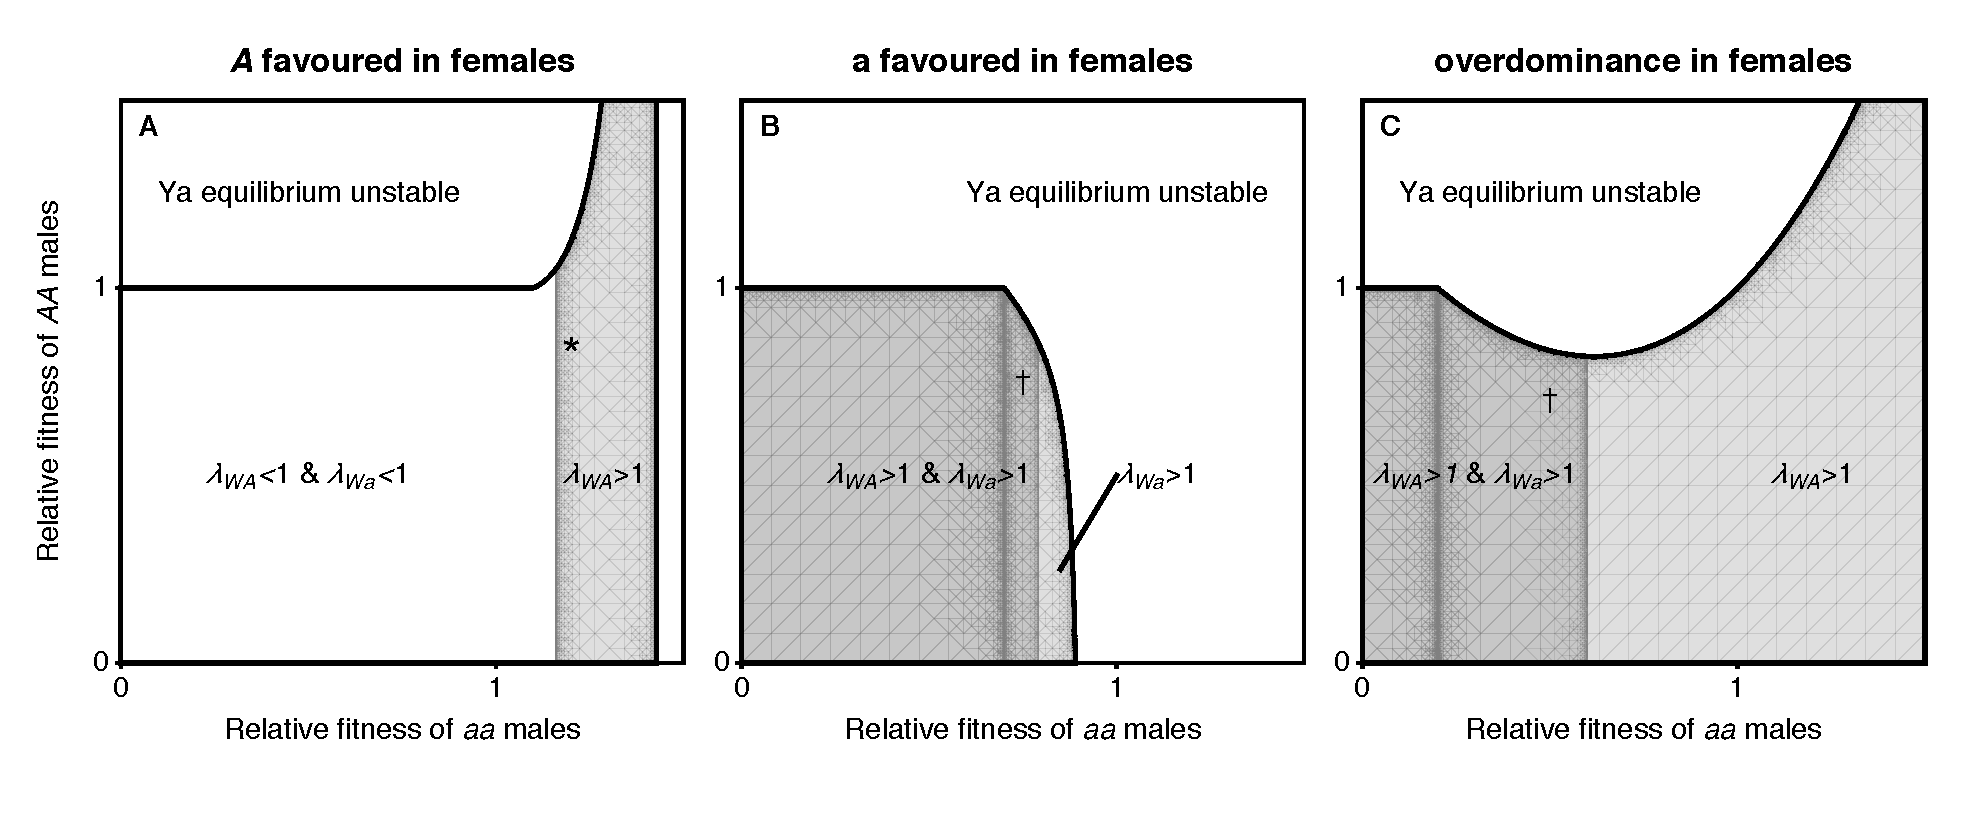
\includegraphics[width=1.25\linewidth]{Region_plot_combined_Mike}}
\DIFdelbeginFL %DIFDELCMD < \centerline{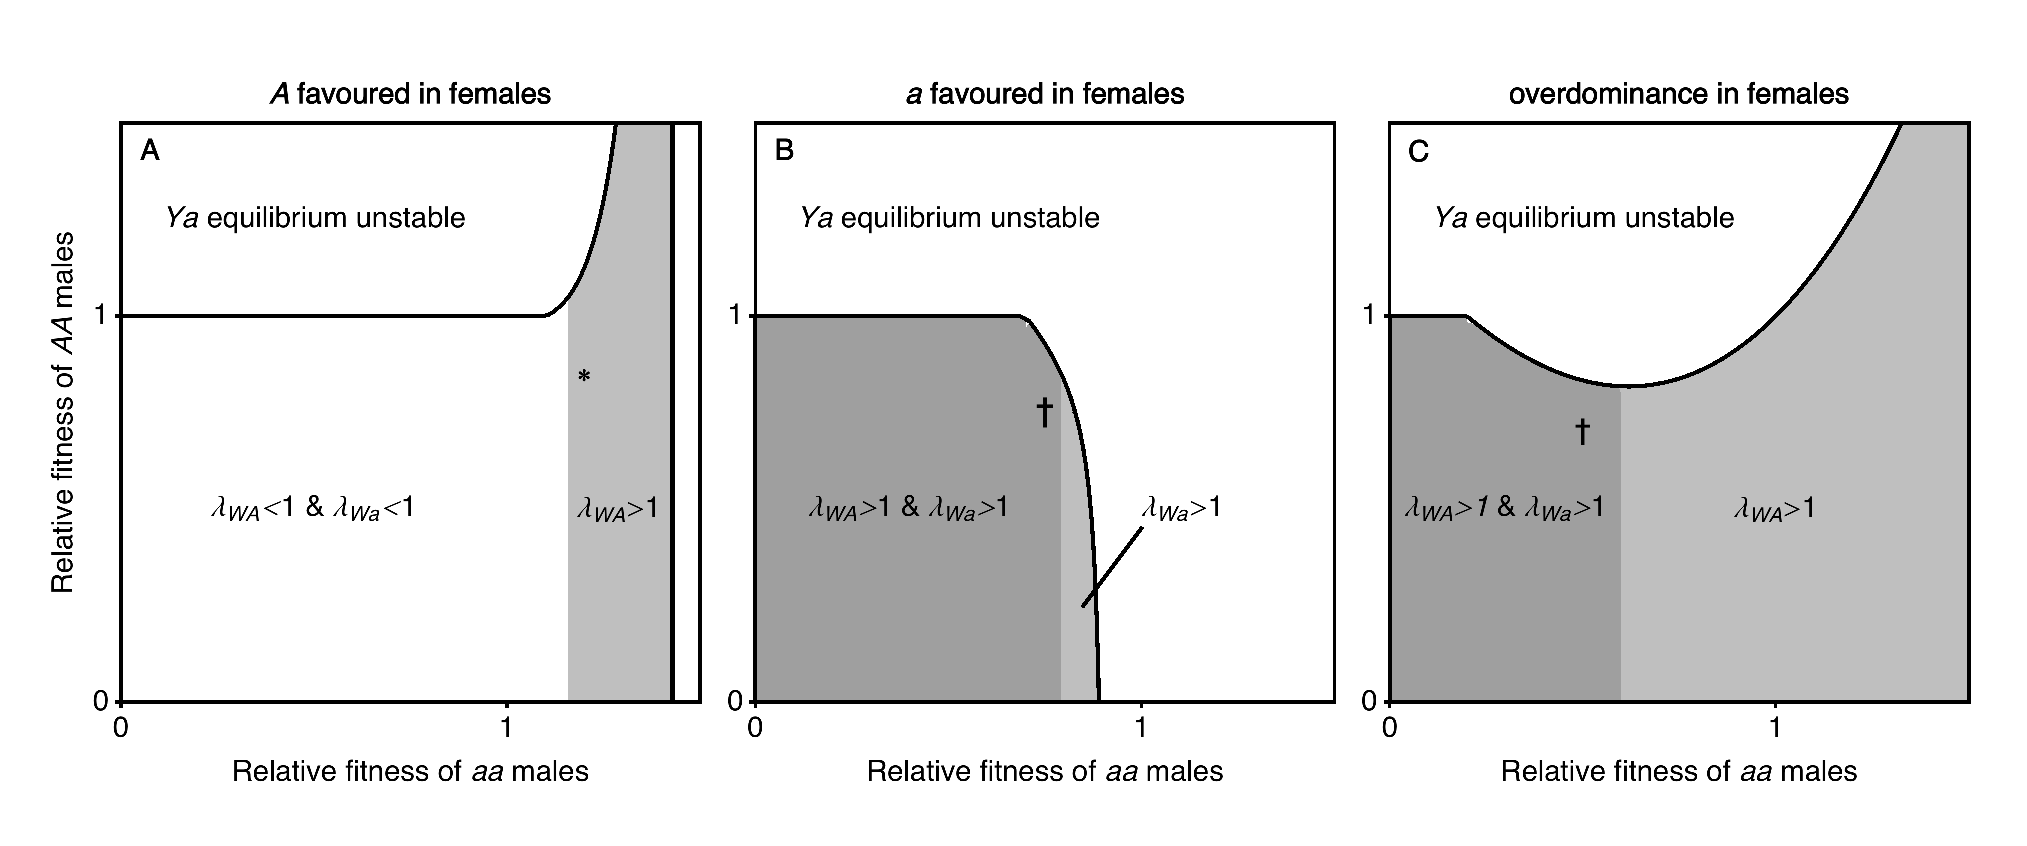
\includegraphics[width=1.4\linewidth, right]{../Plots/Region_plot_combined.eps}}
%DIFDELCMD < %%%
\DIFdelendFL %DIF > \centerline{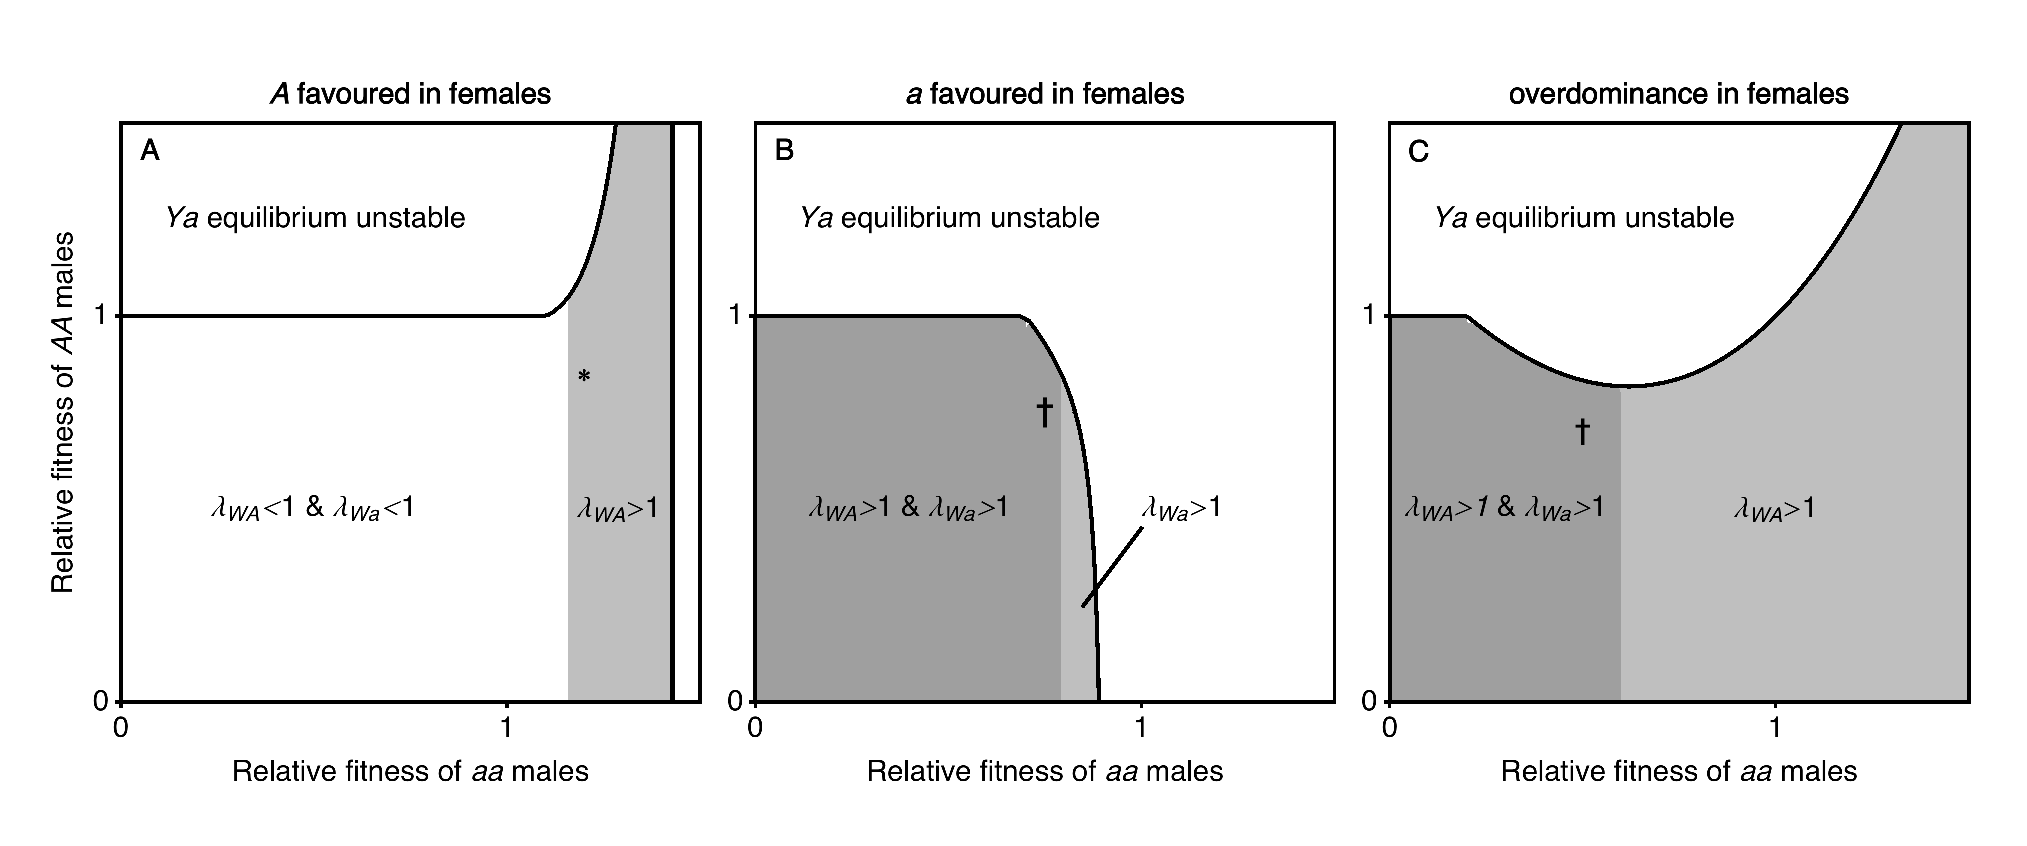
\includegraphics[width=1.4\linewidth, right]{../Plots/Region_plot_combined.eps}}
\caption{
{\bf When the ancestral XY locus is tightly linked to a locus under selection ($r=0$), one or both neo-W haplotypes can spread (no haploid selection).}
We vary the fitness of male homozygotes relative to heterozygotes ($w_{Aa}^\circ=1$) and only consider stable equilibria at which both $\mathbf{A}$ locus alleles are maintained and the $a$ allele is initially fixed on the Y (non-hatched region). 
Here, selection in females can favour the $A$ allele (panel A, $w_{aa}^\female=0.85$, $w_{AA}^\female=1.05$), favour the $a$ allele (panel B, $w_{aa}^\female=1.05$, $w_{AA}^\female=0.85$), or be overdominant (panel C, $w_{aa}^\female=w_{AA}^\female=0.6$). 
If either haplotypic growth rate ($\Lambda_{W'A}^{(XY)}$ or $\Lambda_{W'a}^{(XY)}$) is greater than one, then a rare neo-W allele can spread for, at least, some values of $R>r$ (grey regions). 
The parameter values marked with an asterisk correspond to the fitnesses used in Fig \ref{fig:SexAntagTighter}C. 
%DIF < Where both haplotypic growth rates are greater than one, a neo-W will spread when rare, regardless of linkage with the selected locus (for any $R$). 
\nameref{fig:positionOverdominance} shows the dynamics arising with the parameters marked with a dagger. 
%DIF < Here, there is no haploid selection $t^\circ = \alpha^\circ_\Delta = 0$.
}
\label{fig:regionplots}
\end{figure}

In some cases, both neo-W-$A$ and neo-W-$a$ haplotypes can spread.
For example, when $AA$ individuals have low fitness in females yet the $A$ is polymorphic or fixed on the X background due to overdominance in males (Fig \ref{fig:regionplots}B and \ref{fig:regionplots}C), both neo-W-$A$ and neo-W-$a$ haplotypes produce fewer unfit $AA$ females.
This is true for the neo-W-$A$ haplotype because it can pair with a Y-$a$ haplotype and still be female. 
Whenever both haplotypic growth rates are greater than one, invasion by a neo-W is expected regardless of its linkage with the selected locus (i.e., for any $R$), see \nameref{fig:positionOverdominance} and \nameref{fig:temporalOverdominance} for examples. 
As a consequence, evolution can favor a new sex determination system on a different chromosome ($R = 1/2$), despite the fact that this unlinks the sex-determining locus from the selected locus.

When only one neo-W haplotype has growth rate greater than one (see Fig \ref{fig:regionplots}), a neo-W allele can invade as long as Eq \eqref{eq:lambdasGen} is satisfied, which may require that the recombination rate, $R$, is small enough.
Nevertheless, because we assume here that $r$ is small, these results indicate that a more loosely linked sex-determining region ($r<R$) can spread.
For example, tightly sex-linked loci that experience sexually-antagonistic selection can drive trans-GSD transitions in which the new sex-determining locus is less closely linked ($R>r$, Fig \ref{fig:SexAntagTighter}), but the analysis in \nameref{file:Mathematica} indicates that a new unlinked sex-determining allele ($R=1/2$) cannot invade when selection is purely sexually-antognistic (directional selection in each sex and no haploid selection).

%DIF < %%%%%%%%%%%%%%%%%%%%%%%%%%%%%%%%%%%%%%%%%%%%%%%%%%%%%%%%
%DIF < Tight linkage allows looser sex-linkage to evolve, even in absence of haploid selection
%DIF < %%%%%%%%%%%%%%%%%%%%%%%%%%%%%%%%%%%%%%%%%%%%%%%%%%%%%%%%
\begin{figure}[!h]
\centering
\DIFdelbeginFL %DIFDELCMD < \centerline{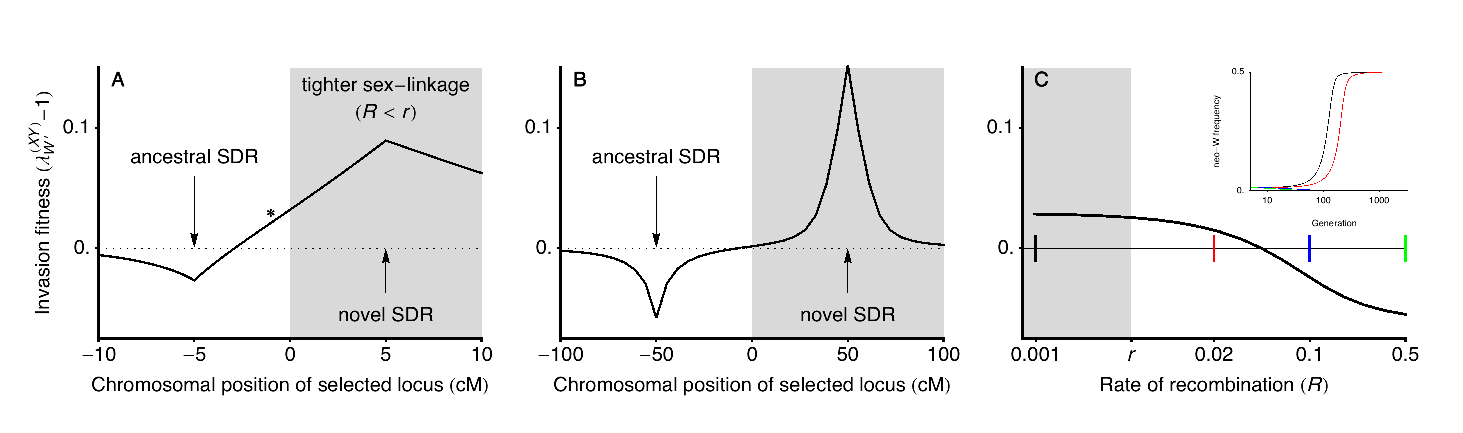
\includegraphics[width=1.4\linewidth, right]{../Plots/PositionPlot_SexAntagTighter.eps}}
%DIFDELCMD < %%%
\DIFdelendFL %DIF > \centerline{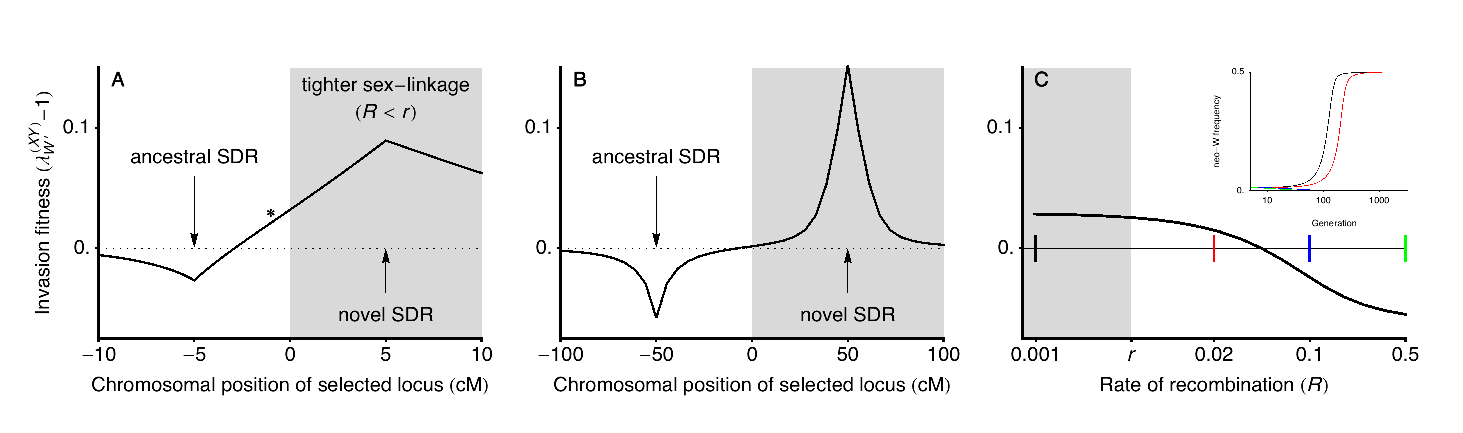
\includegraphics[width=1.4\linewidth, right]{../Plots/PositionPlot_SexAntagTighter.eps}}
\caption{
{\bf Transitions between XY and ZW systems can occur even when the new sex-determining locus is less tightly linked to a locus under sexually-antagonistic selection (no haploid selection).}
In panel A, linkage is initially tight relative to selection and a neo-W can invade even when it is less tightly linked with the selected locus ($r<R$; unshaded region around \textbf{*}).
In panel B, linkage is loose enough relative to selection that the analytical results assuming weak selection hold, and a neo-W allele can only invade when it arises at a locus more tightly linked with the selected locus ($R<r$; shaded region).
In panel C we vary the recombination rate between the neo-W and the selected locus ($R$) for a fixed recombination rate between the ancestral sex-determining locus and the selected locus ($r=0.005$). 
Coloured markers show recombination rates for which the temporal dynamics of invasion are plotted in the inset (frequency of females carrying a neo-W), demonstrating that neo-W alleles can reach fixation if they are more (black) or less (red) closely linked to a locus experiencing sexually-antagonistic selection. 
A very loosely linked neo-W does not spread in this case (blue and green lines overlap and go to 0 in inset). 
Fitness parameters are: $w_{AA}^\female = 1.05$, $w_{aa}^\male = 1.2$, $w_{aa}^\female = w_{AA}^\male = 0.85$, $w_{Aa}^\circ = 1$.
%DIF < ,  $t^\circ = \alpha^\circ_\Delta = 0$.
%DIF < \textcolor{red}{consider removing panel A, which is repeated in Fig 3.}
%DIF < \textcolor{blue}{probably better to remove from panel 3, eh?}
}
\label{fig:SexAntagTighter}
\end{figure}
%DIF < %%%%%%%%%%%%%%%%%%%%%%%%%%%%%%%%%%%%%%%%%%%%%%%%%%%%%%%%

Assuming selection is weak relative to recombination, van Doorn and Kirkpatrick~\cite{vanDoorn:2010hu} showed that invasion by a neo-W allele occurs under the same conditions as its fixation in females.
%DIF < `pseudo-fixation' (at pseudo-fixation the neo-W reaches its maximum frequency among eggs, which is usually 1/2, but can deviate from 1/2 when there is haploid selection before censusing). 
An equivalent analysis is not possible where recombination rates are low. 
However, numerical simulations demonstrate that, with tight sex linkage, neo-Y or neo-W alleles do not necessarily reach fixation in males or females, respectively, which can lead to the stable maintenance of a mixed sex-determining system, in which X, Y, and neo-W alleles all segregate (e.g., \nameref{fig:freqAll}B,C).

From the arguments above we reach:
\vspace{0.5cm}

\noindent\textit{Conclusion 2:}
\textbf{
With tight linkage between a selected locus and the ancestral sex-determining locus ($r\approx0$), trans-GSD transitions (XY $\leftrightarrow$ ZW) can be favoured by selection \textit{even if they weaken sex-linkage} ($r<R$), potentially shifting sex determination to a different chromosome ($R=1/2$). 
Such transitions can also lead to the maintenance of multifactorial sex-determination systems.
}
\vspace{0.5cm} 

\noindent
With haploid selection, Conclusions 1 \& 2 continue to apply (\nameref{app:inv_cond}). 
The parameters for which neo-W-$A$ and neo-W-$a$ haplotypes spread under various forms of haploid selection are plotted in \nameref{fig:regionMaleDrive}, \nameref{fig:regionMaleGS}, \nameref{fig:regionFemaleDrive}, \nameref{fig:regionFemaleGS}.
In particular, we note that adding haploid selection allows shifts in sex determination to a different chromosome ($R=1/2$) even when selection is sexually antagonistic with directional selection in each diploid sex, e.g., \nameref{fig:SexAntagTighterMaleDrive}.  
Furthermore, haploid selection allows variation to be maintained by ploidally-antagonistic selection, under which trans-GSD transitions may also be favoured, \nameref{fig:regionPloidAntag}.
Some cases of XY $\rightarrow$ ZW transitions where $r=0$, $R=1/2$, and selection is ploidally-antagonistic (meiotic drive in males opposed by diploid selection) were studied by Kozielska et al. \cite{Kozielska:2010vm}, who found that sex-ratio biases are reduced during these transitions. 
However, such transitions are not always driven by selection to reduce sex-ratio bias. 
For example, with XY sex determination and haploid selection in females, sex ratios are not ancestrally biased yet a neo-W can invade (\nameref{fig:regionPloidAntag}). 
We further discuss how the spread of neo-sex-determining alleles is influenced by associations with haploid selected loci in the next section. 

\subsection*{Loose linkage with the ancestral sex-determining region}

Here we assume that selection is weak ($s^\circ$, $t^\circ$, $\alpha_{\Delta}^\circ$ of order $\epsilon$, where $\epsilon$ is some number much less than one) and thus implicitly assume that all recombination rates ($r$, $R$ and $\rho$) are large relative to selection.
%DIF < , we denote the leading eigenvalues describing the invasion of a neo-Y ($k=0$) and a neo-W ($k=1$) into an ancestrally XY system by $\lambda_{Y',XY}$ and $\lambda_{W',XY}$, respectively. 
To leading order in selection,

\begin{equation}
\lambda_{Y'}^{(XY)} = 1 + \frac{1}{4}\bar{p}(1-\bar{p}){S_{A}}^2\frac{ \left( r-R \right) }{r R}+O\left(\epsilon^3 \right) 
\label{eq:lambda_neoY}
\end{equation}

\noindent 
and 

\begin{equation}
\lambda_{W'}^{(XY)} =\lambda_{Y'}^{(XY)}+\left[\left(2\alpha_{\Delta}^\male-2\alpha_{\Delta}^\female+t^\male-t^\female \right) \left( \hat{p}^\male_Y-\hat{p}^\male_X \right)/2\right]
+O\left(\epsilon^3 \right)
\label{eq:lambda_neoW}
\end{equation}

\noindent
where $\bar{p}$ is the frequency of $A$, to leading-order (Eq \ref{eq:pAve}), and $S_{A}=(\bar{s}^\male +\alpha_{\Delta}^\male+t^\male) - (\bar{s}^\female+\alpha_{\Delta}^\female+t^\female)$ describes sex differences in selection for the $A$ versus $a$ allele across diploid selection, meiosis, and gametic competition.
The diploid selection term, $\bar{s}^\circ=\big{[} \bar{p}s^\circ+(1-\bar{p})h^\circ s^\circ\big{]} -\big{[} \bar{p}h^\circ s^\circ+(1-\bar{p}) \big{]}$, is the difference in fitness between $A$ and $a$ alleles in diploids of sex $\circ \in \{\female,\male\}$. 
The difference in $A$-allele-frequency among Y-bearing sperm versus X-bearing sperm is, at equilibrium, $\hat{p}^\male_Y-\hat{p}^\male_X=\bar{p}(1-\bar{p})S_{A}(1-2r)/(2r)$. 

%DIF < The new sex-determining allele, $m$, will spread in an XY system if $\lambda_{m}^{(XY)}>1$. 
Eq \eqref{eq:lambda_neoY} demonstrates that, under weak selection, a neo-Y allele will invade an XY system ($\lambda_{Y'}^{(XY)}>1$) if and only if it is more closely linked to the selected locus than the ancestral sex-determining locus (i.e., if $R<r$). 
%DIF < ; note that $\bar{p}(1-\bar{p})S_{A}^2$ is strictly positive as long as $\mathbf{A}$ is polymorphic). 
This echoes our results above where a neo-Y could never invade if $r\approx0$. 
It is also consistent with the results of \cite{vanDoorn:2007eu}, who considered diploid selection only and also found that cis-GSD transitions can only occur when the new sex-determining locus is more closely linked to a locus under sexually-antagonistic selection. 
%DIF < Because tighter linkage between the sex-determining region and a selected locus evolves during these transitions, stronger associations between selected alleles and diploid sexes can build up by selection (e.g., between male-beneficial alleles and the male-determining allele, Y).%, increasing diploid mean fitness (Fig \ref{fig:Combination_MeanFit}). 

\vspace{0.5cm}
\noindent\textit{Conclusion 3A:}\
\textbf{New sex-determining alleles (causing cis-GSD transitions, XY $\leftrightarrow$ XY or ZW $\leftrightarrow$ ZW) are favoured if they arise more closely linked with a locus that experiences (haploid and/or diploid) selection than the ancestral-sex-determining locus ($R<r$).}
\vspace{0.5cm}

\noindent
%DIF < Similarly, a neo-W is typically favoured when it is more closely linked to the selected locus than the ancestral sex-determining region is, ($R<r$).
Similarly, in the absence of haploid selection ($t^\circ=\alpha^\circ_{\Delta}=0$), Eq \eqref{eq:lambda_neoW} indicates that trans-GSD transitions can occur if and only if the new sex-determining locus is more closely linked to a locus under selection, $R<r$, as found by \cite{vanDoorn:2010hu}. 
With haploid selection, a neo-W is also usually favoured when it is more closely linked to the selected locus than the ancestral sex-determining region is, ($R<r$, e.g., Figs \ref{fig:SexAntagTighter}B and \ref{fig:Combination_Centimorgans}); this is true unless the last term in Eq \eqref{eq:lambda_neoW} is negative and dominant over the first, which requires relatively restrictive combinations of selection and recombination parameters. 
For example, with haploid selection, a neo-W will always be favoured if it arises in linkage with a selected locus ($R<1/2$) that is ancestrally autosomal ($r=1/2$, leading to $ \hat{p}^\male_Y-\hat{p}^\male_X =0$). 

\vspace{0.5cm}
\noindent\textit{Conclusion 3B:}\
\textbf{New sex-determining alleles (causing trans-GSD transitions, XY $\leftrightarrow$ ZW) are usually favoured if they arise more closely linked with a locus that experiences (haploid and/or diploid) selection than the ancestral-sex-determining locus ($R<r$).
}
\vspace{0.5cm}

\noindent
However, with haploid selection and some ancestral sex-linkage ($r<1/2$; allowing allele frequency differences on the X and Y), the term in square brackets in Eq \eqref{eq:lambda_neoW} can be positive.
This leads to 

\vspace{0.5cm}
\noindent\textit{Conclusion 3C:}\
\textbf{With haploid selection, new sex-determining alleles (causing trans-GSD transitions, XY $\leftrightarrow$ ZW) can spread even if they arise less closely linked with a locus that experiences selection than the ancestral-sex-determining locus ($r<R$).}
\vspace{0.5cm}

%DIF < %%%%%%%%%%%%%%%%%%%%%%%%%%%%%%%%%%%%%%%%%%%%%%%%%%%%%%%%
%DIF < A neo-W can invade an XY system under a large number of selective regimes
%DIF < %%%%%%%%%%%%%%%%%%%%%%%%%%%%%%%%%%%%%%%%%%%%%%%%%%%%%%%%
\begin{figure}[!h]
\centering
\DIFdelbeginFL %DIFDELCMD < 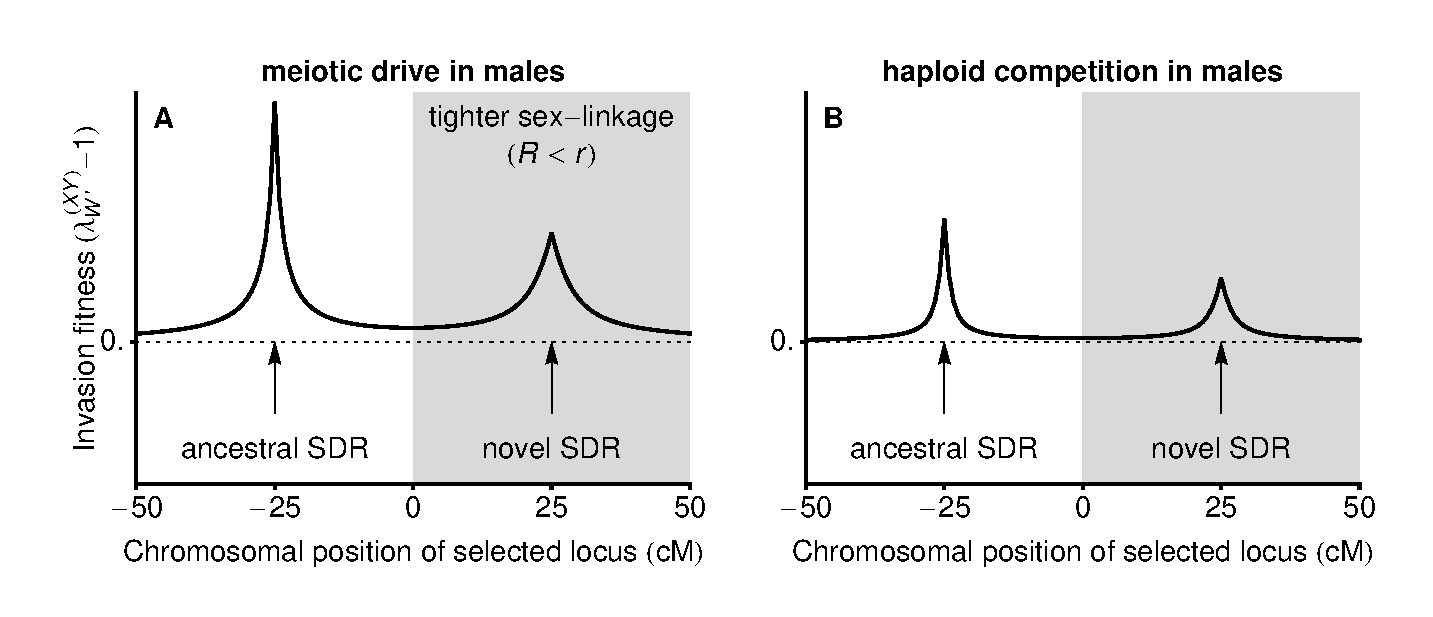
\includegraphics[width=\linewidth]{../Plots/PositionPlot.eps}
%DIFDELCMD < %%%
\DIFdelendFL %DIF > 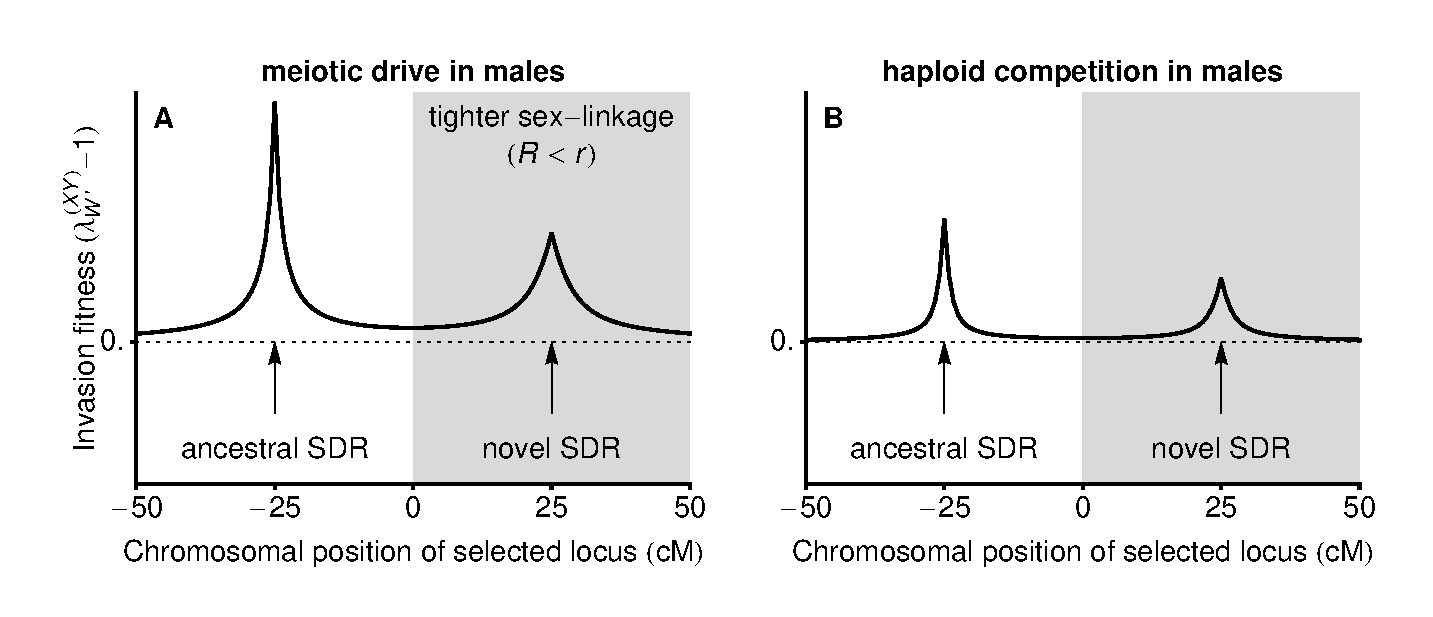
\includegraphics[width=\linewidth]{../Plots/PositionPlot.eps}
\caption{
{\bf Ploidally-antagonistic selection allows a less tightly linked neo-W allele to invade.}
In panel A, male drive ($\alpha^\male_{\Delta} = -1/20$, $t^\circ = \alpha^\female_{\Delta} = 0$) opposes selection in diploids (no sex-differences: $s^\circ = 1/10$, $h^\circ = 7/10$).   
%DIF < , in which case the new sex-determining allele can invade regardless of its linkage with the selected locus ($R$).   
In panel B, gametic competition in males ($t^\male = -1/10$, $t^\female = \alpha^\circ_{\Delta} = 0$) opposes selection in diploids (sex-differences: $s^\male = 3/20$, $s^\female = 1/20$, $h^\circ = 7/10$).
In either case the new sex-determining allele can invade regardless of $R$, even when linkage to the selected locus is reduced (white regions).
}
\label{fig:Combination_Centimorgans}
\end{figure}
%DIF < %%%%%%%%%%%%%%%%%%%%%%%%%%%%%%%%%%%%%%%%%%%%%%%%%%%%%%%%

To clarify the parameter space under which neo-W alleles spread despite looser linkage with the selected locus ($R>r$), we focus on cases where dominance coefficients are equal in the two sexes, $h^\female=h^\male$, and haploid selection only occurs in one sex (e.g., during male meiosis only).
Table \ref{tab:specialcases} then gives the conditions required for unlinked ($R=1/2$) neo-W invasion when there is some ancestral sex-linkage ($r<1/2$; e.g., the selected locus is on the ancestral sex chromosome and the novel sex-determining locus arises on an autosome). 
These special cases indicate that neo-W invasion occurs for a large fraction of the parameter space, even though the neo-W uncouples the sex-determining locus from a locus under selection. 
Fig \ref{fig:Combination_Centimorgans} then demonstrates that under these conditions neo-W alleles can spread when they are more loosely \textit{or} more closely linked to the locus that experiences haploid selection, i.e., Conclusions 3B and 3C (c.f., Fig \ref{fig:SexAntagTighter}A for diploid sexually-antagonistic selection alone). 
%DIF < When the neo-W is more closely linked to the haploid selected locus its invasion increases (or creates anew) sex-ratio bias (Fig \ref{fig:SexRatioBad}A).
%DIF < Under the same selection scenario (drive in males), a neo-Y would invade an ancestrally ZW system
%DIF <  shows that when a neo-W invades that increases linkage with a haploid selected locus, it biases the sex-ratio.
%DIF < , while those that decrease sex-linkage equalize the sex-ratio. 
%DIF < When sex-linkage decreases ($R>r$), neo-W alleles can benefit from Y-associated alleles that have higher fitness in the female diploid phase but then dissociate from these alleles through recombination before any subsequent haploid selection. 

%DIF < When there is no gametic competition and meiotic drive is in one sex only, an unlinked neo-W can invade as long as the same allele is favoured during diploid selection in males and females ($s^\female s^\male>0$, see Fig \ref{fig:Combination_Centimorgans}A and Fig \ref{fig:SexRatioBad}B). %, which is 50\% of the parameter space. 
%DIF < When there is no meiotic drive and gametic competition occurs in one sex only, an unlinked neo-W can invade as long as the same allele is favoured in male and female diploid selection and there are sex differences in selection of one type (e.g., $s^\female(s^\male-s^\female)>0$, see Fig \ref{fig:Combination_Centimorgans}B). %, which is 25\% of the parameter space. 
%DIF < These special cases indicate that neo-W invasion occurs for a relatively large fraction of the parameter space, even if the neo-W uncouples the sex-determining locus from a locus under selection. 
\DIFdelbegin %DIFDELCMD < 

%DIFDELCMD < %%%
\DIFdelend \begin{table}[!ht]
\centering
\smallskip
\caption{Invasion conditions for a neo-W allele at an unlinked locus ($R=1/2$) into an ancestral XY system with linkage ($r<1/2$) and a single form of haploid selection}
\begin{tabular}{l l c }
\hline\hline
Scenario &  Assumptions & neo-W spreads ($\lambda_{W'}^{(XY)}>1$) if \\ [0.5ex] \hline
%DIF <   $r=1/2$, $R<1/2$ & Always \\ [0.5ex] \hline
%DIF <   $r<1/2$, $R=1/2$ &  \\ [0.5ex] \hline
\noalign{\vskip 1mm}
  male drive only & $h^\male=h^\female$, $t^\female=t^\male=\alpha^\female_{\Delta}=0$ & $s^\female s^\male>0$ \\ [0.5ex]
 female drive only & $h^\male=h^\female$, $t^\female=t^\male=\alpha^\male_{\Delta}=0$ & $s^\female s^\male>0$ \\ [0.5ex]
 male gametic competition only &  $h^\male=h^\female$, $t^\female=\alpha^\female_{\Delta}=\alpha^\male_{\Delta}=0$ & $s^\female(s^\male-s^\female)>0$ \\ [0.5ex]
  female gametic competition only & $h^\male=h^\female$, $t^\male=\alpha^\female_{\Delta}=\alpha^\male_{\Delta}=0$ & $s^\male(s^\female-s^\male)>0$ \\ [0.5ex]
  \hline \hline
  \label{tab:specialcases}
 \end{tabular}
\end{table}

We can also compare transitions in genetic sex-determination where sex-ratio bias increases, decreases, or remains equal. 
For example, if there is meiotic drive in males only ($\alpha^\male_\Delta \neq 0$, $\alpha^\female_\Delta=0$), without gametic competition ($t^\female=t^\male=0$) the zygotic sex ratio is initially biased only when the ancestral sex-determining system is XY (Figs \ref{fig:model_outline}B and \ref{fig:SexRatioBad}A) and not ZW (Figs \ref{fig:model_outline}B and \ref{fig:SexRatioBad}B).
%DIF < If the ancxestral sex-determining system is ZW, the zygotic sex ratio will be 1:1 because diploid sex is determined by the proportion of Z-bearing versus W-bearing eggs and meiosis in females is fair (Fig \ref{fig:Combination_Turnover}D).
If Fisherian sex-ratio selection were dominant, we would thus expect a difference in the potential for XY to ZW and ZW to XY transitions. 
%DIF < However, to leading order with selection weak relative to recombination, we find that sex-ratio selection favours the spread of a neo-W by an amount equl to the spread of a neo-Y into a ZW system (relabeling XY as the heterogametic sex and reversing the labels of males and females in Table \ref{tab:specialcases})
However, invasion by a neo-W allele into an XY system and invasion by a neo-Y allele into a ZW system occur under the same conditions ($\lambda_{Y'}^{(XY)} = \lambda_{W'}^{(ZW)}$ and $\lambda_{W'}^{(XY)}=\lambda_{Y'}^{(ZW)}$, at least to order $\epsilon^2$), implying that,
%DIF <  surprisingly,
\vspace{0.5cm}

\noindent\textit{Conclusion 4:}
\textbf{When selection is weak relative to recombination, \DIFaddbegin \DIFadd{trans-GSD transitions in }\DIFaddend the presence of haploid selection \DIFdelbegin \DIFdel{equally favors the spread of new sex determination systems that reduce }\DIFdelend \DIFaddbegin \DIFadd{are favoured as often and as strongly whether they erase ancestral }\DIFaddend sex-ratio bias (benefiting from Fisherian sex ratio selection) or \DIFdelbegin \DIFdel{that }\DIFdelend generate \DIFdelbegin \DIFdel{a }\DIFdelend sex-ratio bias (benefiting from associations with selected alleles). } 
\vspace{0.5cm}
%DIF < \noindent\textcolor{red}{\textit{Conclusion 3:}
%DIF < \textbf{when selection is weak relative to recombination, sex-ratio selection is exactly equal in magnitude to the selection imposed by associations with selected alleles. } }
%DIF < %\textcolor{red}{[new result]}
%DIF < \vspace{0.5cm}

\noindent For example, in Fig \ref{fig:SexRatioBad}A neo-W alleles invade an ancestral-XY system where females are initially rare, equalizing the sex ratio (as occurs in \cite{Kozielska:2010vm}).
However, Fig \ref{fig:SexRatioBad}B shows that a neo-Y can invade the resulting ZW system under the same conditions. 
When $R<1/2$, the invading neo-Y becomes associated with the male meiotic drive allele and the zygotic sex ratio evolves to become male-biased (as occurs in \cite{Ubeda:2015fx}, beginning from ESD). 
In this case, the neo-Y spreads because it is often found in males and can, if it carries the driven allele $a$, benefit from haploid selection in males (Fig \ref{fig:SexRatioBad}B).

%DIF < %%%%%%%%%%%%%%%%%%%%%%%%%%%%%%%%%%%%%%%%%%%%%%%%%%%%%%%%
%DIF < sex-ratio selection is not a good predictor of neo-W invasion into an XY system
%DIF < %%%%%%%%%%%%%%%%%%%%%%%%%%%%%%%%%%%%%%%%%%%%%%%%%%%%%%%%
\begin{figure}[!h]
\centering
\DIFdelbeginFL %DIFDELCMD < 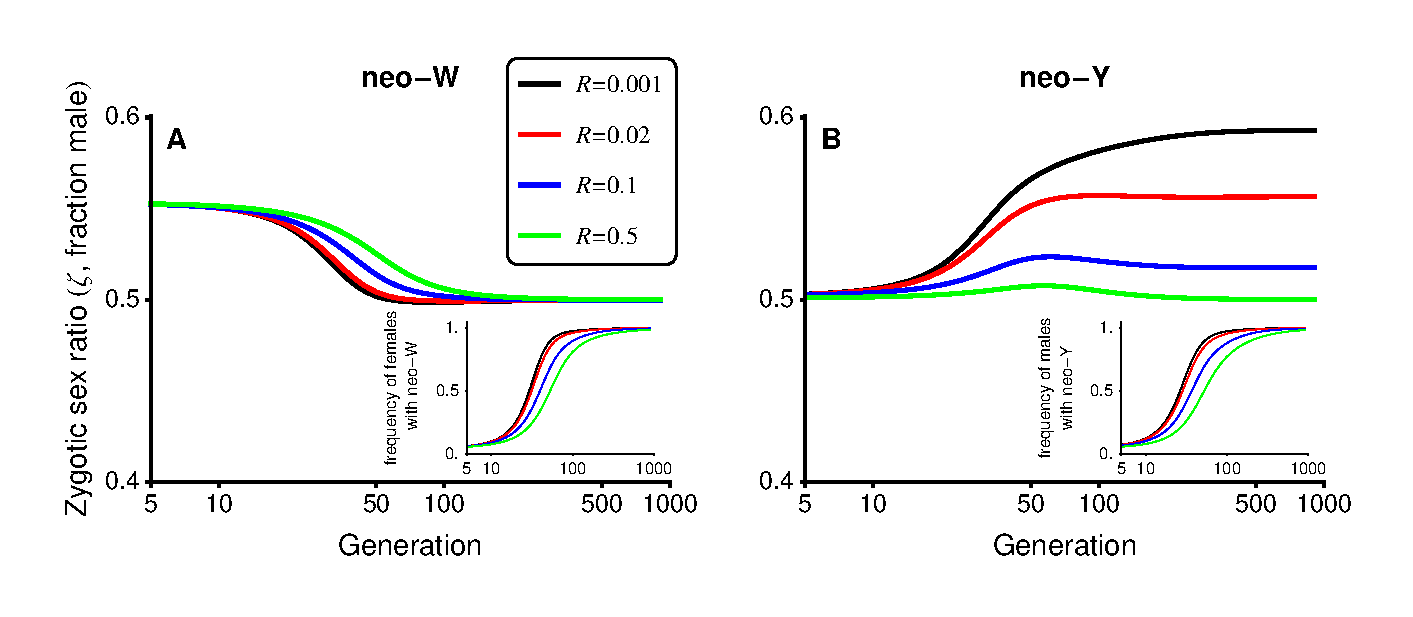
\includegraphics[width=\linewidth]{../Plots/Temporal_SR.eps}
%DIFDELCMD < %%%
\DIFdelendFL %DIF > 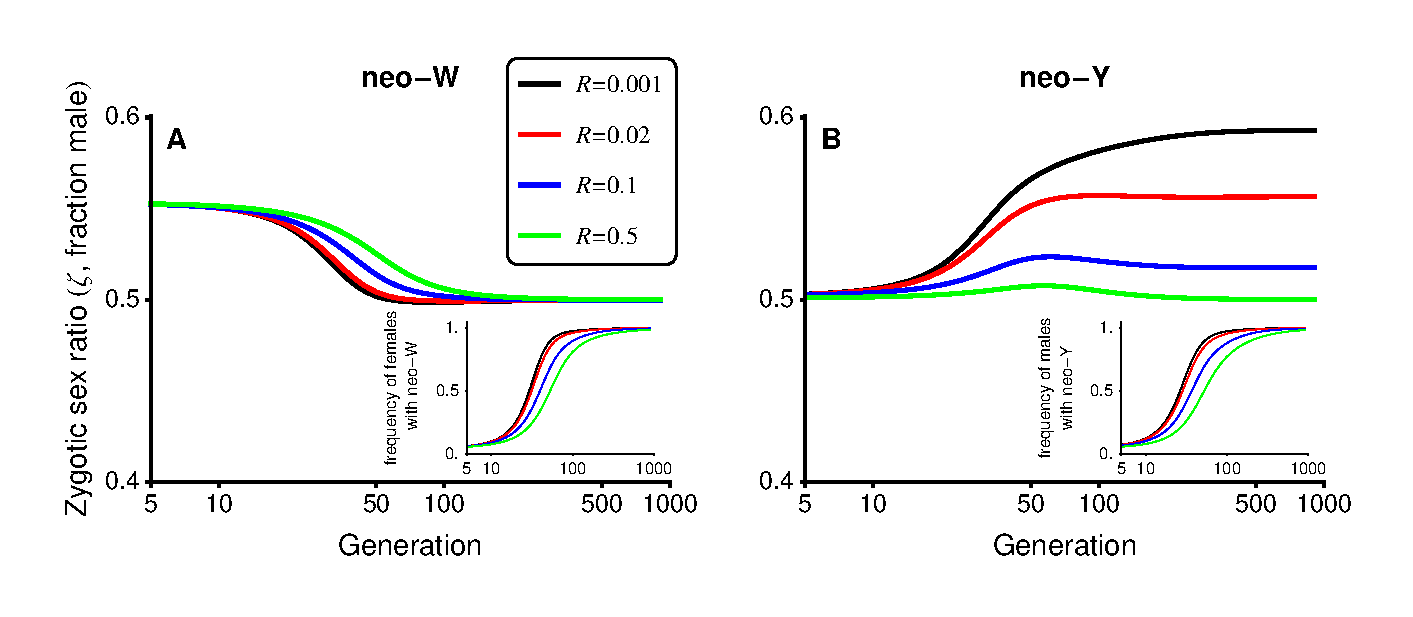
\includegraphics[width=\linewidth]{../Plots/Temporal_SR.eps}
\caption{
{\bf Fisherian sex-ratio selection alone is not a good predictor of turnover between sex-determining systems.}
In this figure, selection is ploidally antagonistic with haploid selection favouring the $a$ allele during male meiosis.
In panel A, male meiotic drive in an ancestral XY system causes a male bias (see Fig \ref{fig:model_outline}B), allowing a neo-W to invade and replace the ancestral sex-determining system (inset shows the frequency of females carrying a neo-W), which balances the zygotic sex ratio.
In panel B, male drive in an ancestral ZW system has no effect on the zygotic sex ratio (50:50 at generation 0), yet a neo-Y can invade and replace the ancestral sex-determining system (inset shows the frequency of males carrying a neo-Y). 
%DIF < When $R<1/2$, the neo-Y becomes associated with the allele favoured by drive, causing the zygotic sex ratio to become biased, hence the frequency of the neo-Y at pseudo-fixation can be higher than $0.5$ (inset).
Parameters:  $s^\female =s^\male = 0.2$, $h^\female = h^\male = 0.7$, $t^\female = t^\male = \alpha^\female_\Delta = 0$, $\alpha^\male_\Delta = -0.1$, $r=0.02$.
}
\label{fig:SexRatioBad}
\end{figure}
%DIF < %%%%%%%%%%%%%%%%%%%%%%%%%%%%%%%%%%%%%%%%%%%%%%%%%%%%%%%%

%DIF < 
%DIF < As selection becomes stronger (or linkage becomes tighter), this symmetry between sex-ratio selection and haploid selection is lost, causing differences in the strength of selection favouring the two heterogametic transitions (compare red to black near -25cM and 25 cM in Fig \ref{fig:Combination_Centimorgans}). \textcolor{red}{normalise fitness in sexually antagonistic case}
%DIF < 
%DIF < Why can new sex-determining regions invade when they are more loosely linked to selected loci ($R>r$)?  
%DIF < Consider first the case where both sex-determining-loci are linked to the selected locus ($r<R<1/2$). 
%DIF < In an ancestral-XY system, haploid selection in males can facilitate the spread of a neo-W because the zygotic sex ratio is ancestrally male biased and the W produces more of the rarer sex (Fig \ref{fig:SexRatioBad}A). 
%DIF < A new sex determining region can also, however, benefit from becoming more associated with drive. 
%DIF < For example in an ancestral-ZW system with the same selection regime (haploid selection in males), a neo-Y can spread despite the fact that the zygotic sex is initially even; in this case, the neo-Y spreads because it is often found in males and can, if it carries the driven allele $a$, benefit from haploid selection in males (Fig \ref{fig:SexRatioBad}B). 
\DIFdelbegin %DIFDELCMD < 

%DIFDELCMD < %%%
\DIFdelend While equalizing the sex ratio and benefiting from associations with selected alleles are two primary reasons why haploid selection spurs sex chromosome transitions, more complex situations also arise.  
For example with $R=1/2$ in Fig \ref{fig:SexRatioBad}B (green curve), the neo-Y allele spreads despite the fact that it cannot benefit from drive because free recombination moves it randomly between driven and non-driven backgrounds.  
Nevertheless, the unlinked neo-Y can spread because males bearing it more often carry the non-driven allele $A$ and have higher average diploid fitness compared to ZZ males, which bear a high frequency of the driven allele, $a$, from their mothers.

\subsection*{Environmental sex determination}

We next consider the case where the new sex-determining allele, $m$, causes sex to be determined probabilistically or by heterogeneous environmental conditions (environmental sex determination, ESD).
In particular, we assume individuals carrying allele $m$ develop as females with probability $k\in(0,1)$.
%DIF < \textcolor{red}{In our deterministic model this means the fraction female is exactly $k$, even when $m$ is rare (exploring the effect of the variance induced by ESD would also be interesting).}
In our deterministic model this means the fraction female in the subpopulation containing $m$ is exactly $k$, even when $m$ is rare (i.e., ESD does not introduce any additional variance in sex determination). 
We also assume that the environmental conditions that determine sex do not differentially affect the fitness of males versus females. 
Such correlations can favour environmental sex-determining systems by allowing each sex to be produced in the environment in which it has highest fitness; in the absence of these correlations previous theory would predict that ESD is favoured when it produces more equal sex ratios than the ancestral system (see reviews by~\cite{Charnov:1982wg,Bull:1983vi,West:2009we}). 
%DIF < (e.g., maternal condition, mate quality, age, or host size)  

The characteristic polynomial determining the leading eigenvalue (\DIFdelbegin \DIFdel{equations }\DIFdelend \DIFaddbegin \DIFadd{Eqs }\DIFaddend \ref{eq:recursions}) does not factor for ESD ($0<k<1$) as it does for a neo-Y ($k=0$) or neo-W ($k=1$) allele. 
We therefore focus on weak selection here, where the leading eigenvalue is

\begin{equation}
\begin{split}
\lambda_{ESD'}^{(XY)} =& 1 + \frac{{(1-2k)}^2}{4}\bar{p}(1-\bar{p}){S_{A}}^2\frac{r-R}{r R} \\
&+\frac{k(\hat{p}^\male_Y-\hat{p}^\male_X)}{2}\left[ k \left(2\alpha_{\Delta}^\male-2\alpha_{\Delta}^\female+t^\male-t^\female \right) -2(1-k)S_{A}\right]+O\left(\epsilon^3\right).
\end{split}
\label{eq:lambda_ESD_k}
\end{equation}

\noindent
This reduces to $\lambda_{Y'}^{(XY)}$ when $k=0$ and $\lambda_{W'}^{(XY)}$ when $k=1$. 
\DIFdelbegin %DIFDELCMD < 

%DIFDELCMD < %%%
%DIF < Under Fisherian sex-ratio selection, autosomal modifiers favour equal investment in male and female offspring, i.e., a 1:1 sex ratio~\cite{Fisher:1930wy,Charnov:1982wg,West:2009we}. 
%DIF < A novel environmental sex-determiner that causes half of its carriers to become female and half to become male ($k=1/2$) will be in males half of the time and in females half of the time (like an autosome).
%DIF < In addition, these novel sex-determination alleles equalize the sex ratio and therefore one might expect them to be favoured by Fisherian sex-ratio selection when the resident sex ratio is biased.
%DIF < However, assuming weak selection, we find that the growth rate of a rare, dominant offspring-controlled neo-ESD allele that produces males or females with equal probability ($k=1/2$) is
\DIFdelend Of particular interest are ESD mutations that cause half of their carriers to develop as females and half as males ($k=1/2$), creating equal sex ratios.
The spread of such mutations is determined by
\begin{equation}
\lambda_{ESD'}^{(XY)} =1+ \frac{1}{2}\frac{(\lambda_{Y'\rvert R=1/2}^{(XY)}-1) + (\lambda_{W'\rvert R=1/2}^{(XY)}-1)}{2} + O\left(\epsilon^3\right),
%DIF < V_A \frac{r}{1-2r}  \frac{s_{f} \left( s^\male - 3 s^\female\right) }{8 {\left( s_{f} + s_{m} \right)}^2} t_{m}^2.
\label{eq:lambda_ESD}
\end{equation}
\noindent
where $\lambda_{Y'\rvert R=1/2}^{(XY)}$ and $\lambda_{W'\rvert R=1/2}^{(XY)}$ represent $\lambda_{Y'}^{(XY)}$ and $\lambda_{W'}^{(XY)}$ when evaluated at $R=1/2$ (\DIFdelbegin \DIFdel{Equations }\DIFdelend \DIFaddbegin \DIFadd{Eqs }\DIFaddend \ref{eq:lambda_neoY} and \ref{eq:lambda_neoW}).
That is, ESD with $k=1/2$ behaves as if the $\mathbf{M}$ and $\mathbf{A}$ loci were unlinked, regardless of the actual value of $R$.
This is because sex is randomized each generation in individuals bearing the $m$ allele, preventing associations from building up between it and alleles at locus $\mathbf{A}$. 
Eq \eqref{eq:lambda_ESD} shows that the ESD mutation gets half of the fitness of a feminizing mutation (neo-W) and half of the fitness of a masculinizing mutation (neo-Y), but only has an effect one half of the time (the other half of the time it produces the same sex as the ancestral system would have). 
As discussed above, $\lambda_{Y'\rvert R=1/2}^{(XY)}$ is necessarily less than or equal to one when selection is weak (Conclusion 3A), but $\lambda_{W'\rvert R=1/2}^{(XY)}$ can be greater than one if there is haploid selection (see Conclusion 3C).
That is, with haploid selection, an allele causing environmental-sex-determination can invade an ancestrally-XY system because it generates females that are either rare or have high fitness, in the same manner as a neo-W (likewise, ESD invades a ZW system for the same reasons that a neo-Y can).
%DIF < An important result from Eq \eqref{eq:lambda_ESD} is that ESD can invade if there is haploid selection. 
%DIF < When evaluated at $R=1/2$, $\Lambda_{Y',XY}$ is necessarily less than one, but $\Lambda_{W',XY}$ can be greater than one if there is haploid selection, as discussed above. 
%DIF < Previous studies where ESD is favoured have typically assumed that environmental conditions (e.g., maternal condition, mate quality, age, or host size) can differentially affect the fitness of males versus females such that ESD invades because it allows sex determination to depend on the environment \citep[reviewed in][]{Charnov:1982wg,Bull:1983vi,West:2009we}. 
%DIF < Here, ESD mutations can spread because they generate females that are either rare or have high fitness, in the same manner as a neo-W. 

Significantly, Eq \eqref{eq:lambda_ESD} is the same whether ESD is invading an ancestrally XY or ZW system (because $\lambda_{Y'}^{(XY)} = \lambda_{W'}^{(ZW)}$ and $\lambda_{W'}^{(XY)} = \lambda_{Y'}^{(ZW)}$).
Thus, focusing solely on Fisherian selection to equalize the sex-ratio does not fully explain GSD to ESD transitions.
For example, when the ancestral sex-determining system is XY the sex ratio is biased by male haploid selection.
When the ancestral sex-determining system is ZW the sex ratio is not biased.
Nevertheless, ESD is equally likely to invade both XY (through $\lambda_{W'}^{(XY)}$) and ZW (through $\lambda_{Y'}^{(ZW)}$) systems, equalizing the zygotic sex ratio in the former case but not in the latter. 
%DIF < This is again because haploid selection can facilitate the turnover of sex chromosomes either through sex-ratio biases or through associations between the new sex determining region with selected alleles. 
%DIF < With weak selection, these two forces are nearly equal in strength. 
In addition, we note that ESD may not invade, even if the sex ratio is initially biased (e.g., with drive in males only, $r<1/2$, $h^\female=h^\male$, and $s^\female s^\male<0$, then $\lambda_{W'}^{(XY)}<1$, see Table \ref{tab:specialcases}). 
We conclude that, as with neo-W and neo-Y mutations:
\vspace{0.5cm}

\noindent\textit{Conclusion 5:}
\textbf{
Transitions from genetic to environmental sex-determination are not straightforwardly predicted by selection to balance the zygotic sex ratio when haploid selection is present. 
}
%DIF < \textcolor{red}{[new result]}

%DIF < \textcolor{red}{
%DIF < Somehow need to add two further conclusions suggested by review 2:
%DIF < \vspace{0.5cm}
%DIF < \\
%DIF < \noindent\textit{Conclusion 6: sex-antagonism and tighter sex linkage not required for transitions.}
%DIF < \vspace{0.5cm}
%DIF < \\
%DIF < \noindent\textit{Conclusion 7: haploid selection makes conditions for transitions permissive.}
%DIF < \vspace{0.5cm}
%DIF < \\
%DIF < \noindent Or are these evident from the first 5 conclusions?
%DIF < }
\DIFdelbegin %DIFDELCMD < 

%DIFDELCMD < %%%
\DIFdelend %DIF > %%%%%%%%%%%%%%%%
\section*{Discussion}
%DIF > %%%%%%%%%%%%%%%%

New sex-determination systems are typically expected to spread when they equalise the sex ratio and/or when they increase linkage with loci that experience sex-differences in selection~\cite{Blaser2012, vanDoorn2014re}.
In accordance with the latter mechanism, we find that sex-differences in selection at the haploid stage can favour cis- or trans-GSD transitions that tighten sex-linkage (Conclusion 3A \&3B). 
%DIF < , as exemplified in~\cite{Ubeda:2015fx} for ESD-GSD transitions. 
Contrary to this expectation, however, we find that trans-GSD transitions can be favoured that loosen linkage with the sex-determining locus, either when linkage is initially tight (Conclusions 1 \& 2, Figs \ref{fig:regionplots} \& \ref{fig:SexAntagTighter}) or when there is haploid selection (Conclusion 3C, Figs \ref{fig:Combination_Centimorgans} \& \ref{fig:SexRatioBad}). 
Furthermore, we show that the spread of new sex-determination systems is not dominated by selection to balance the sex ratio (Conclusions 4 \& 5, Fig \ref{fig:SexRatioBad}). 

%DIF < We find that the spread of new sex-determining systems cannot be simply predicted from their effect on the sex ratio. 
On the one hand, sex-ratio biases caused by haploid selection can facilitate trans-GSD transitions or transitions from genetic to environmental sex determination~\cite{Kozielska:2010vm}. 
For instance, alleles favoured by haploid selection in males often become associated with the Y allele, which leads to an ancestral male-biased zygotic sex ratio.
This male bias increases the potential for a neo-W or ESD allele to invade (Table \ref{tab:haplotype_growth}), equalizing the sex ratio (e.g., see Fig \ref{fig:SexRatioBad}B, for related examples see~\cite{Kozielska:2010vm}).
%DIF < We find that sex-ratio biases caused by haploid selection can also affect transitions between sex-determining systems (e.g., see $\zeta$ terms in Table \ref{tab:haplotype_growth}). 
%DIF < However, the neo-W may not equalize the sex ratio (e.g., if the driving allele also drives in females or affects competition among eggs)
On the other hand, sex-ratio selection can be overwhelmed by additional selective effects, preventing a neo-W or ESD allele from invading, even if it would balance the sex ratio (e.g., when selection also acts in opposite directions in male and female diploids, Table \ref{tab:specialcases}).
%DIF < and equalizing the sex ratio.
Indeed, transitions between sex-determining systems can generate stronger sex-ratio biases (e.g., Fig \ref{fig:SexRatioBad}A and step 1 in~\cite{Ubeda:2015fx}).
Significantly, with weak selection, we find that there is no difference in conditions allowing XY to ZW and ZW to XY transitions (Conclusion 4) 
even when haploid selection always acts in the same sex (e.g., males).  
That is, the sex-ratio bias created by male haploid selection facilitates the spread of a neo-W allele into an XY system to the same degree that male haploid selection drives the spread of a neo-Y into a ZW system with a 1:1 sex ratio (Fig \ref{fig:SexRatioBad}).
%DIF < Thus, haploid selection can favour trans-GSD transitions both via sex-ratio selection and via selection on alleles associated with the new sex-determining allele, and these selective pressures are often predicted to be of equal magnitude. 


%DIF < Our results indicate that haploid selection could be an important factor driving the evolution of new sex-determining systems. 
Because both Fisherian selection to equalize the sex ratio and the benefits of hitchhiking with driven alleles can facilitate transitions among sex chromosome systems, we predict that haploid selection should increase the lability of sex determination systems.
Even in animal and plant species that have much larger and more conspicuous diploid phases than haploid phases, many loci have been shown to experience haploid selection through gamete competition and/or meiotic drive~\cite{Mulcahy:1996ha,JOSEPH:2004haa, Lalanne2004,Ubeda:2005gw,Fishman2005,Leppala2008,Leppala2013,Didion2015,Didion2016,Lindholm:2016cw}, which can generate biased sex-ratios~\cite{Jaenike:2001vb,Burt:2006,Lloyd:1974tz,Conn:1981uw,Stehlik:2005ul,Stehlik:2006to,Field:2012fd,Field:2013cc}. 
In animals, a relatively small proportion of all genes are thought to be expressed and selected during competition in animal sperm~\cite{Zheng:2001fi,JOSEPH:2004haa,Vibranovski:2010et}.
Nevertheless, recent studies have demonstrated that sperm competition, even within a single ejaculate, can alter haploid allele frequencies and increase offspring fitness~\cite{Immler:2014im,Alavioon2017}.
Expression in the gamete is not required for haploid selection if the fitness of a gamete depends on its ability to condense DNA~\cite{Immler2018}. 
Furthermore, expression during gamete production often underlies systems of meiotic drive~\cite{Tau2007,Cocquet2012,Helleu2016}, which may be a common form of haploid selection in animals~\cite{Bachtrog2018}.
In plants, competition among gametophytes may be particularly important. 
It is estimated that 60-70\% of all genes are expressed in the male gametophyte, and these genes exhibit stronger signatures of selection than randomly-chosen genes~\cite{Borg:2009jpa,Arunkumar:2013iq,Gossmann:2014dua}. 
Furthermore, artificial selection pressures applied to male gametophytes are known to cause a response to selection (e.g.,~\cite{Hormaza:1996cv,Ravikumar:2003uo,Hedhly:2004iv,Clarke:2004ir}). 

%DIF < HAPLOID SELECTION (genomic location of haploid selected loci and comparative patterns) 
Linking haploid expression with the evolution of sex-determination, a recent transcriptome analysis in \textit{Rumex} shows that pollen-biased expression (relative to expression in flower buds or leaves) is enhanced among XY-linked genes compared to autosomal genes or compared to hemizygous genes that are only linked to the X 
\cite{Sandler264382}. 
In addition, Y-linked genes are over-expressed relative to X-linked genes in pollen (but not in flower buds or leaves). 
This suggests that the spread of neo-Y chromosomes in this clade could have been favoured through linkage with haploid selected genes rather than those under sexually antagonistic selection. 
%DIF < maybe add a flag here for switching to clade-level expectations:

%DIF < In general, we predict that haploid selection increases lability of sex-determining systems, particularly because haploid selection can cause transitions that increase or decrease sex-linkage (Conclusion 2A \& 2B, e.g., the final state of the red line in Fig \ref{fig:SexRatioBad}B is the starting state in Fig \ref{fig:SexRatioBad}A). 
Frequent turnovers driven by haploid selection may help to explain the relative rarity of heteromorphic sex chromosomes in plants.
If haploid selection is strong but selective differences between male and female diploids are weak, we specifically predict that trans-GSD transitions are favoured more strongly than cis-GSD transitions, with transitions to ESD intermediate (e.g., with $|\bar{s}^\male - \bar{s}^\female| << |\alpha_\Delta^\male - \alpha_\Delta^\female + t^\male - t^\female|$ we have $\lambda_{W'}^{(XY)} > \lambda_{Y'}^{(XY)}$; Eq \ref{eq:lambda_neoW}). 
Among the relatively few dioecious clades in which multiple species have well characterized sex chromosomes~\cite{Ming:2011iy}, trans-GSD transitions have been inferred in \textit{Silene} subsection \textit{Otites}~\cite{Slancarova:2013dq} and in \textit{Salicaceae}~\cite{Pucholt2015,Pucholt2017}.
Assuming that transitions from dioecy to hermaphroditism (equal parental investment in male and female gametes) are favoured in a similar manner to the ESD examined here (equal probability of zygotes developing as males or females), our results suggest that competition among haploid pollen could drive transitions between dioecy and hermaphroditism, which are frequent in plants~\cite{Kafer2017, Goldberg2017}. 
To further examine this link, future theory could also include inbreeding, which is an important consideration during transitions between dioecy and hermaphroditism~\cite{Charlesworth1978}. 
Future empirical studies could look for evidence of haploid selection acting on former sex chromosomes in hermaphroditic species (e.g., a study such as \cite{Sandler264382} on ancestral, rather than derived, sex chromosomes). 

New sex-determining alleles have previously been shown to spread when they arise in linkage with loci that experience sex differences in selection because beneficial associations build up between alleles that determine sex and alleles that are favoured in that sex~\cite{vanDoorn:2007eu,vanDoorn:2010hu,Ubeda:2015fx,Muralidhar2018}. 
In support of this hypothesis, researchers have identified genes on recently derived sex chromosomes that might be under sexually-antagonistic selection~\cite{Lindholm:2002dw,Tripathi:2009cw,Roberts2009,Ser:2010iq}. 
However, we show that, if selected loci are tightly linked to the ancestral sex-determining locus, they can drive trans-GSD transitions that reduce sex-linkage (Conclusions 1 \& 2), thus widening the range of genomic locations where selection could be driving observed trans-GSD transitions.
In addition, we find that polymorphic sex determining systems (X, Y, and neo-W alleles all segregating) can be maintained when a selected locus is tightly linked to the ancestral sex-determining system (e.g., \nameref{fig:freqAll}B and \nameref{fig:freqAll}C), which is not possible with loose linkage~\cite{vanDoorn:2010hu}. 
This pair of conclusions apply in cases with or without haploid selection. 

Our tight linkage result, in particular the prediction that invasion can lead to polymorphic sex determination, is consistent with empirical data from species in which new feminizing mutations are found segregating with ancestral XY loci.
For example, in the platyfish (\textit{Xiphophorus maculatus}), X,Y, and W alleles segregate at one locus (or two closely-linked loci) near to potentially sexually-antagonistic genes for pigmentation and sexual maturity~\cite{Kallman1965,Kallman1968, Volff2001, Schultheis2006}.
Furthermore, several rodent species maintain feminizing alleles along with the ancestral X and Y sex-determination alleles (reviewed in~\cite{Fredga1994}). 
In nine \textit{Akadon} rodent species, it appears that male-determining-\textit{sry} expression is suppressed by an autosomal feminizing allele (a neo-W allele), creating XY females~\cite{Bianchi2002,Sanchez2010}. 
XY females have increased fitness relative to XX females~\cite{Hoekstra2001}. 
However, it is not yet clear whether loci linked to the feminizing factor or the ancestral Y cause this effect. 
Most convincingly, in \textit{Mus minutoides}, females can have XX, XX$^\ast$ or X$^\ast$Y genotypes~\cite{Veyrunes2010}. 
Previous theory would predict that the dominant X$^\ast$ chromosome (potentially an autosome that has fused with the sex chromosome) harbours female beneficial alleles, driving its spread. 
However, XX and XX$^\ast$ females have similar fitness, whereas X$^\ast$Y female fitness is enhanced~\cite{Saunders2014,Saunders2016, Veyrunes2017}. 
Although Y-linkage of female-beneficial alleles is counterintuitive, our model suggests that it can be stably maintained when linkage is initially tight between the sex determining region and the selected locus, subsequently favoring new feminizing mutations, which would be a parsimonious explanation for the spread of feminizing alleles in this case. 

%DIF < Limitation 1: DEGENERATE Y
Our models assume that sex-determining alleles do not experience direct selection except via their associations with sex and selected alleles.
However, in some cases, there may be significant degeneration around the sex-limited allele (Y or W) in the ancestral sex-determining region because recessive deleterious mutations and/or deletions accumulate in the surrounding non-recombining regions~\cite{Rice:1996ke,Charlesworth:2000cc,Bachtrog:2006ed,Marais:2008hm}. 
During trans-GSD transitions, but not cis-GSD transitions, any recessive deleterious alleles linked to the Y or W are revealed to selection in YY or WW individuals~\cite{Bachtrog:2014bx}. 
This phenomenon was studied by van Doorn and Kirkpatrick (2010)~\cite{vanDoorn:2010hu}, who found that degeneration can prevent fixation of a neo-W or a neo-Y allele, leading to a mixed sex-determining system where the ancestral and new sex-determining loci are both segregating. 
However, they noted that very rare recombination events around the ancestral sex-determining locus can allow the completion of trans-GSD transitions.  
%DIF < While not explicitly studied, we also predict that Y or W degeneration would prevent fixation of the new sex-determining genes considered here.
Degeneration around the Y or W could explain why trans-GSD transitions are not observed to be much more common than cis-GSD transitions despite the fact that our models demonstrate that they are favoured under a wider range of conditions, especially with haploid selection. 
For example, there are a dozen sex chromosome configurations among Dipteran species but only one transition between male and female heterogamety~\cite{Vicoso:2015hf}, but Y degeneration or absence is also very common among \textit{Diptera}~\cite{Vicoso:2015hf}. 

%DIF < Limitation 3: don't consider m alleles with similar k to ancester, no ancestral ESD considered
In this study, we have only considered new sex-determining alleles of large effect. 
However, we expect similar selective forces to act on masculinizing/feminizing alleles of weaker effect.
For example, small effect masculinizing/feminizing alleles within a threshold model of sex determination can be favoured when linked to loci that experience sexually-antagonistic selection~\cite{Muralidhar2018}. 
These results echo those for large-effect neo-Y/neo-W alleles~\cite{vanDoorn:2007eu,vanDoorn:2010hu}.
It should be noted, however, that the dynamics of sex-determining alleles with very weak effect will be influenced by genetic drift, which itself has been shown to bias transitions towards epistatically-dominant sex-determining systems when there is no direct selection \cite{Veller2017}.

%DIF < Limitation 2: TWO ALLELE DRIVE
%DIF < Another simplification that we made is that meiotic drive involves only a single locus with two alleles. 
%DIF < However, many meiotic drive systems involve an interaction with another locus at which alleles may `suppress' the action of meiotic drive \citep[][]{Burt:2006,Lindholm:2016cw}.
%DIF < Thus, the dynamics of meiotic drive alleles can be heavily dependent on the interaction between two loci and the recombination rate between them, which in turn can be affected by sex-linkage if there is reduced recombination between sex chromosomes~\cite{Hurst:1991uh}.
%DIF < Furthermore, in some cases, a driving allele may act by killing any gametes that carry a `target' allele at another locus, in which case there can be fertility effects that alter the equilibrium frequency of a meiotic drive allele~\cite{Holman:2015en}. 
%DIF < In polygamous mating systems, the intensity of pollen/sperm competition can depend on the density of males available to donate pollen/sperm, which can itself depend on the sex ratio~\cite{Taylor:2002wu}. 
%DIF < In terms of our model, this implies that the strength of gametic competition ($t^\male$) may both determine and be determined by the sex ratio. 
%DIF < How the evolution of new sex-determining mechanisms could be influenced by two-locus meiotic drive and/or by ecological feedbacks under different mating systems remains to be studied.
\DIFdelbegin %DIFDELCMD < 

%DIFDELCMD < %%%
\DIFdelend %DIF > %%%%%%%%%%%%%%%%%
\section*{Conclusion}
%DIF > %%%%%%%%%%%%%%%%%

We have shown that tight sex-linkage and haploid selection can drive previously unexpected transitions between sex-determining systems.
In particular, both can select for new sex-determining loci that are more loosely linked to loci under selection (Conclusions 2 \& 3C). 
In addition, haploid selection can cause transitions in GSD analogous to those caused by purely sexually-antagonistic selection, eliminating the need for differences in selection between male and female diploids (Conclusion 3A, 3B \& 3C).
We conclude that haploid selection should be considered as a pivotal factor driving transitions between sex-determining systems. 
Further, transitions involving haploid selection can eliminate or generate sex-ratio biases; to leading order, selection to balance the sex ratio and the benefits of hitch-hiking with haploid selected alleles, leading to a biased sex ratio, are of equal magnitude (Conclusions 4 \& 5). 
Overall, our results suggest several novel scenarios under which new sex-determining systems are favoured, which could help to explain why the evolution of sex-determining systems is so dynamic. 

% For figure citations, please use "Fig" instead of "Figure".

% Place figure captions after the first paragraph in which they are cited.

% Results and Discussion can be combined.

% Place tables after the first paragraph in which they are cited.

%PLOS does not support heading levels beyond the 3rd (no 4th level headings).

%DIF > %%%%%%%%%%%%%%%%%
\section*{Supporting information}
%DIF > %%%%%%%%%%%%%%%%%

\paragraph*{S1 File.}
\label{file:Mathematica}
{\bf Supplementary \textit{Mathematica} file.}  This file can be used to re-derive our results and generate figures. 

\DIFaddbegin \paragraph*{\DIFadd{S2 File.}}
\label{file:MathematicaCDF}
{\bf \DIFadd{Supplementary }\textit{\DIFadd{Mathematica}} \DIFadd{file in CDF form.}}  \DIFadd{This file can be used to re-derive our results and generate figures with a free online viewer (}\hyperref[www.wolfram.com/cdf-player/]{www.wolfram.com/cdf-player/}\DIFadd{). 
}

\paragraph*{\DIFadd{S3 File.}}
\label{file:MathematicaPDF}
{\bf \DIFadd{Supplementary }\textit{\DIFadd{Mathematica}} \DIFadd{file in PDF form.}}  \DIFadd{This file can be used to see how we have derived our results and have generated figures with any PDF viewer. 
}

\DIFaddend \paragraph*{S1 Table}
\label{tab:chisubstitutions}
{\bf Substitutions for different loci orders assuming no interference.}

\paragraph*{S2 Table}
\label{tab:meanfitnesses}
{\bf Mean fitnesses and zygotic sex ratio in the resident population ($M$ fixed, XY sex determination). }

\paragraph*{S1 Appendix.}
\label{app:recurs}
{\bf Recursion equations and complete model description.} 

\paragraph*{S2 Appendix.}
\label{app:eq_stab}
{\bf Equilibria and stability conditions when $M$ allele is fixed. } 

\paragraph*{S3 Appendix.}
\label{app:inv_cond}
{\bf Invasion conditions for the $m$ allele.} 

% Include only the SI item label in the paragraph heading. Use the \nameref{label} command to cite SI items in the text.
\paragraph*{S1 Fig.}
\label{fig:positionOverdominance}
{\bf With overdominance, loci near to the ancestral sex-determining locus ($r\approx0$) can favour neo-W alleles that are less tightly linked ($R>r$).} 
In panels A and B, the $a$ allele is favoured in females ($w_{aa}^\female=1.05$, $w_{Aa}^\circ=1$, $w_{AA}^\female=0.85$) and selection in males is overdominant ($w_{aa}^\male=w_{AA}^\male=0.75$).
In panels C and D, selection in males and females is overdominant ($w_{aa}^\female=w_{AA}^\female=0.6$, $w_{aa}^\male=0.5$, $w_{AA}^\male=0.7$, $w_{Aa}^\circ=1$).
There is no haploid selection $t^\circ = \alpha^\circ_\Delta = 0$.
These parameters are marked by daggers in Fig \ref{fig:regionplots}B and C, which show that neo-W invasion is expected for any $R$ ($\Lambda_{W'A}^{(XY)},\Lambda_{W'a}^{(XY)}>1$) if the $a$ allele is nearly fixed on the Y (black lines in this figure; not stable for $r>>0$). 
Equilibria where the $A$ allele is more common among Y-bearing male gametes can also be stable and allow neo-W invasion for these parameters (blue lines). 
%DIF < The weak selection approximation holds when all recombination rates are large relative to selection (around 0 in panels A and C), in which case, in the absence of haploid selection, neo-W alleles should spread if and only if they are more tightly linked to the selected locus (positive invasion fitness if and only if the selected locus is in the grey region). 
%DIF < However, when recombination rates are small (panels B and D and when the selected locus is near the SDRs in all panels), this weak selection prediction can break down. 

\paragraph*{S2 Fig.}
\label{fig:temporalOverdominance}
{\bf Following invasion by a neo-W allele, there can be a complete transition to a new sex-determining system, maintenance of both ancestral-XY and neo-ZW sex determining systems, or loss of the new sex-determining allele.}  
Here, we plot the frequency of the neo-W allele among female gametes.
%DIF < ; as the neo-W reaches frequency $0.5$, polymorphism at the ancestral XY locus is lost with Y becoming fixed such that sex is determined only be the ZW allele carried by a female gamete. 
Panels A, C and D show cases where a steady state is reached with the neo-W at a frequency below $0.5$, in which case ancestral-X and Y alleles also both segregate. 
In all cases, we assume that the $a$ allele is initially more common than the $A$ allele on the Y background (Y-$a$ is fixed when $r=0$). 
When $r>0$ (panels B and D), Y-$A$ haplotypes created by recombination can become more common than Y-$a$ haplotypes as the neo-W spreads.
In B, this leads to loss of the neo-W and the system goes to an equilibrium with X-$a$ and Y-$A$ haplotypes fixed (equilibrium $A'$), such that all females have the high fitness genotype $aa$ and all males are $Aa$. 
For the parameters in B, neo-W alleles have negative invasion fitness when the Y-$A$ haplotype is ancestrally more common than Y-$a$ (compare blue to black curves in \nameref{fig:positionOverdominance}A and  \nameref{fig:positionOverdominance}B near the ancestral sex-determining locus). 
In contrast, the neo-W is not lost in panel D as it is favoured regardless of whether Y-$A$ or Y-$a$ haplotypes predominate (again, compare blue to black curves in \nameref{fig:positionOverdominance}C and  \nameref{fig:positionOverdominance}D). 
%DIF < Fitness parameters are the same as in \nameref{fig:positionOverdominance}; in panels A and B the $a$ allele is favoured in females ($w_{aa}^\female=1.05$, $w_{Aa}^\circ=1$, $w_{AA}^\female=0.85$) while there is overdominance in males ($w_{aa}^\male=w_{AA}^\male=0.75$) and in panels C and D, there is overdominance in both sexes ($w_{aa}^\female=w_{AA}^\female=0.6$, $w_{aa}^\male=0.5$, $w_{AA}^\male=0.7$, $w_{Aa}^\circ=1$). 
%DIF < These parameters are marked by a dagger in Fig \ref{fig:regionplots}. 
%DIF < Here, there is no haploid selection $t^\circ = \alpha^\circ_\Delta = 0$.

\paragraph*{S3 Fig.}
\label{fig:SexAntagTighterMaleDrive}
{\bf  When there is sexually-antagonistic selection and haploid selection, a neo-W allele may invade for any $R$.}
Panel A shows that the invasion fitness of a neo-W is positive, even when $r<R$ (unshaded region).
In panel B, we vary the recombination rate between the neo-W and the selected locus ($R$) for a fixed recombination rate between the ancestral sex-determining locus and the selected locus ($r=0.005$).
Coloured markers show recombination rates for which the temporal dynamics of neo-W invasion are plotted in panel C (black $R=0.001$, red $R=0.02$, blue $R=0.1$, green $R=0.5$). 
The diploid selection parameters used in this plot are the same as in Fig \ref{fig:SexAntagTighter}. 
There is also meiotic drive in males favouring $a$ ($\alpha_{\Delta}^\male=-0.08$), this full set of parameters is marked by an asterisk in \nameref{fig:regionMaleDrive}A.
When $R=0.5$ (green curve), the neo-W does not reach fixation and X, Y, Z, and W alleles are all maintained in the population, see \nameref{fig:freqAll}C.

\paragraph*{S4 Fig.}
\label{fig:regionMaleDrive}
{\bf Parameters for which neo-W-$A$ and neo-W-$a$ haplotypes spread when there is male meiotic drive at a locus that is tightly linked to the ancestral XY locus ($r=0$).}
This figure is equivalent to Fig \ref{fig:regionplots} but with meiotic drive in males.
%DIF < We vary the fitness of male homozygotes relative to heterozygotes ($w_{Aa}^\circ=1$) and only consider stable equilibria at which both $\mathbf{A}$ locus allele are maintained and the $a$ allele is initially fixed on the Y, region outlined. 
In panels A-C, meiotic drive in males favours the $a$ allele ($\alpha_{\Delta}^\male=-0.16$), creating male-biased sex ratios and generally increasing $\Lambda_{W'A}^{(XY)}$ and $\Lambda_{W'a}^{(XY)}$. 
By contrast, $\Lambda_{W'A}^{(XY)}$ and $\Lambda_{W'a}^{(XY)}$ tend to be reduced when meiotic drive in males favours the $A$ allele ($\alpha_{\Delta}^\male=0.16$), panels D-F. 
%DIF < We consider three forms of selection in females: directional selection in favour of the $A$ allele (panels A and D, $w_{aa}^\female=0.85$, $w_{AA}^\female=1.05$), direction selection in favour of the $a$ allele (panels B and E, $w_{aa}^\female=1.05$, $w_{AA}^\female=0.85$), and overdominance (panels C and F, $w_{aa}^\female=w_{AA}^\female=0.6$).

\paragraph*{S5 Fig.}
\label{fig:regionMaleGS}
{\bf Parameters for which neo-W-$A$ and neo-W-$a$ haplotypes spread when there is male gametic competition at a locus that is tightly linked to the ancestral XY locus ($r=0$).}
This figure is equivalent to Fig \ref{fig:regionplots} but with gametic competition in males.
%DIF < Diploid selection parameters ($w_{ij}^\circ$) are the same as those in \nameref{fig:regionMaleDrive}. 
The $a$ allele is favoured during male gametic competition in Panels A-C ($w_{a}^\male=1.16$, $w_{A}^\male=1$), which creates male biased sex ratios and increases $\Lambda_{W'A}^{(XY)}$ and $\Lambda_{W'a}^{(XY)}$. 
By contrast, $\Lambda_{W'A}^{(XY)}$ and $\Lambda_{W'a}^{(XY)}$ tend to be reduced when the $A$ allele is favoured during male gametic competition, panels D-F.
Compared to the meiotic drive parameters in \nameref{fig:regionMaleDrive}, the effect of these male gametic competition parameters on the sex ratio is smaller. 
For example, in \nameref{fig:regionMaleDrive}A-C, the ancestral sex ratio is $\alpha^\male=0.58$ at equilibrium (B) and in panels A-C of this plot, the ancestral sex ratio is $w_{a}^\male/(w_{A}^\male+w_{a}^\male)=0.537$ at equilibrium (B). 

\paragraph*{S6 Fig.}
\label{fig:regionFemaleDrive}
{\bf Parameters for which neo-W-$A$ and neo-W-$a$ haplotypes spread when there is female meiotic drive at a locus that is tightly linked to the ancestral XY locus ($r=0$).}
This figure is equivalent to Fig \ref{fig:regionplots} but with meiotic drive in females.
%DIF < Diploid selection parameters ($w_{ij}^\circ$) are the same as those in \nameref{fig:regionMaleDrive} and \nameref{fig:regionMaleGS}. 
The $a$ allele is favoured by meiotic drive in females in Panels A-C ($\alpha_{\Delta}^\female=-0.16$), which increases $\Lambda_{W'a}^{(XY)}$ and decreases $\Lambda_{W'A}^{(XY)}$. 
Female meiotic drive in favour of the $A$ allele (panels D-F, $\alpha_{\Delta}^\female=-0.16$) has the opposite effect. 

\paragraph*{S7 Fig.}
\label{fig:regionFemaleGS}
{\bf Parameters for which neo-W-$A$ and neo-W-$a$ haplotypes spread when there is female gametic competition at a locus that is tightly linked to the ancestral XY locus ($r=0$).}
This figure is equivalent to Fig \ref{fig:regionplots} but with gametic competition in females.
%DIF < Diploid selection parameters ($w_{ij}^\circ$) are the same as those in \nameref{fig:regionMaleDrive}, \nameref{fig:regionMaleGS}, and \nameref{fig:regionFemaleDrive}. 
The $a$ allele is favoured during female gametic competition in females in Panels A-C ($w_{a}^\female=1.16$, $w_{A}^\female=1$), which increases $\Lambda_{W'a}^{(XY)}$ and decreases $\Lambda_{W'A}^{(XY)}$. 
The $A$ allele is favoured during gametic competition in panels D-F ($w_{a}^\female=1$, $w_{A}^\female=1.16$), giving the opposite effect on $\Lambda_{W'a}^{(XY)}$ and $\Lambda_{W'A}^{(XY)}$. 

\paragraph*{S8 Fig.}
\label{fig:regionPloidAntag}
{\bf Ploidally-antagonistic selection can drive the spread of neo-W alleles. }
A-D show when each of the neo-W haplotypes invades an internally stable equilibrium with $a$ fixed on the Y (found by setting $r=0$).
The y-axis shows directional selection in diploids of both sexes, $s^\female=s^\male$, and the x-axes show sex-limited drive, $\alpha_\Delta^\circ$, or haploid competition, $t^\circ$.
The top left and bottom right quadrants therefore imply ploidally-antagonistic selection (and these are the only places where neo-W haplotypes can invade).
Dominance is equal in both sexes, $h^\female=h^\male=3/4$. 
E-F show the temporal dynamics of neo-W frequency in females with parameters given by the asterisks in the corresponding A-D plot, with $r=1/200$, for four different $R$.
Black $R=1/1000$, Red $R=2/100$, Blue $R=1/10$, Green $R=1/2$.  

\paragraph*{S9 Fig.}
\label{fig:freqAll}
{\bf Pseudo-fixation of neo-W or maintenance of multiple sex-determining alleles. }
The curves show the frequencies of the neo-W (red), ancestral Y (blue), and $A$ allele (black) among female gametes (solid curves) and among male gametes (dashed curves). 
In panel A, there is a complete transition from XY sex determination (XX-ZZ females and XY-ZZ males) to ZW sex determination (YY-ZW females and YY-ZZ males).  
In panels B and C a polymorphism is maintained at both the ancestral XY locus and the new ZW locus, such that there are males with genotypes XY-ZZ and YY-ZZ and females with genotypes XX-ZZ, XX-ZW, XY-ZW, and YY-ZW. 
In panel A, selection is ploidally-antagonistic with drive in males (parameters as in the green curve in Fig \ref{fig:SexRatioBad}B).
In panel B, there is overdominance in both sexes and no haploid selection (parameters as in the green curve in \nameref{fig:temporalOverdominance}C).
In panel C, there is sexually-antagonistic selection in diploids with drive in males (parameters as in the green curve in \nameref{fig:regionMaleDrive}C).
In all cases, the initial equilibrium frequency has $a$ near fixation on the Y.

%DIF > %%%%%%%%%%%%%%%%%
\section*{Acknowledgments}
%DIF > %%%%%%%%%%%%%%%%%
We thank Georgy Sandler and Stephen Wright for sharing their results with us \DIFdelbegin \DIFdel{, }\DIFdelend and we thank Bret Payseur \DIFdelbegin \DIFdel{and three anonymous reviewers }\DIFdelend for helpful comments on \DIFaddbegin \DIFadd{a previous version of }\DIFaddend this manuscript. 
%This project was supported by the Natural Sciences and Engineering Research Council of Canada (CGS-D 6564 to MMO; RGPIN-2016-03711 to SPO). 

\nolinenumbers

% Either type in your references using
% \begin{thebibliography}{}
% \bibitem{}
% Text
% \end{thebibliography}
%
% or
%
% Compile your BiBTeX database using our plos2015.bst
% style file and paste the contents of your .bbl file
% here. See http://journals.plos.org/plosone/s/latex for 
% step-by-step instructions.
%DIF <  
\DIFdelbegin %DIFDELCMD < \bibliography{sex_chromosomes}
%DIFDELCMD < %%%
\DIFdelend 

%DIF < \newpage
%DIF < 
%DIF < \setcounter{equation}{0}
%DIF < \renewcommand{\theequation}{S1.\arabic{equation}}
%DIF < 
%DIF < \section*{S1 Appendix}
%DIF < 
%DIF < \subsection*{Recursion equations}
%DIF < 
%DIF < 
%DIF < In each generation we census the genotype frequencies in male and female gametes/gametophytes (hereafter, gametes) between meiosis (and any meiotic drive) and gametic competition. 
%DIF < At this stage we denote the frequencies of X- and Y-bearing gametes from males and females $x_{i}^{\circ}$ and $y_{i}^{\circ}$.
%DIF < The superscript $\circ \in \{\male,\female\}$ specifies the sex of the diploid that the gamete came from. 
%DIF < The subscript $i\in\{1,2,3,4\}$ specifies the genotype at the selected locus $\mathbf{A}$ and at the novel sex-determining locus $\mathbf{M}$, where $1=AM$, $2=aM$, $3=Am$, and $4=am$. 
%DIF < The gamete frequencies from each sex sum to one, $\sum_{i}x_{i}^{\circ}+y_{i}^{\circ}=1$. 
%DIF < 
%DIF < Competition then occurs among gametes of the same sex (e.g., among eggs and among sperm separately) according to the genotype at the $\mathbf{A}$ locus ($w_{1}^\circ=w_{3}^\circ=w_{A}^\circ$, $w_{2}^\circ=w_{4}^\circ=w_{a}^\circ$, see Table \ref{tab:fitnesstable}).
%DIF < The genotype frequencies after gametic competition are $x_{i}^{\circ,s}= w_{i}^{\circ}x_{i}^{\circ}/\bar{w}_{H}^{\circ}$ and $y_{i}^{\circ,s}= w_{i}^{\circ}y_{i}^{\circ}/\bar{w}_{H}^{\circ}$, where $\bar{w}_{H}^{\circ}=\sum_{i} w_{i}^{\circ}x_{i}^{\circ}+w_{i}^{\circ}y_{i}^{\circ}$ is the mean fitness of male ($\circ=\male$) or female ($\circ=\female$) gametes. 
%DIF < 
%DIF < Random mating then occurs between gametes to produce diploid zygotes.
%DIF < %To shorten notation we now use index $i$ (and $j$) to denote the alleles at both the $\mathbf{A}$ and $\mathbf{M}$ loci and label $MA=1$, $Ma=2$, $mA=3$, and $ma=4$, such that $i,j\in\{1,2,3,4\}$.
%DIF < The frequencies of XX zygotes are then denoted as $xx_{ij}$, XY zygotes as $xy_{ij}$, and YY zygotes as $yy_{ij}$, where $\mathbf{A}$ and $\mathbf{M}$ locus genotypes are given by $i,j\in\{1,2,3,4\}$, as above. 
%DIF < In XY zygotes, the haplotype inherited from an X-bearing gamete is given by $i$ and the haplotype from a Y-bearing gamete is given by $j$. 
%DIF < In XX and YY zygotes, individuals with diploid genotype $ij$ are equivalent to those with diploid genotype $ji$; for simplicity, we use $xx_{ij}$ and $yy_{ij}$ with $i\neq j$ to denote the average of these frequencies, $xx_{ij}=(x_{i}^{\female,s}x_{j}^{\male,s}+x_{j}^{\female,s}x_{i}^{\male,s})/2$ and $yy_{ij}=(y_{i}^{\female,s}y_{j}^{\male,s}+y_{j}^{\female,s}y_{i}^{\male,s})/2$. 
%DIF < 
%DIF < 
%DIF < Denoting the $\mathbf{M}$ locus genotype by $b \in \{MM, Mm, mm\}$ and the $\mathbf{X}$ locus genotype by $c \in \{XX, XY, YY\}$, zygotes develop as females with probability $k_{bc}$. 
%DIF < Therefore, the frequencies of XX females are given by $xx_{ij}^{\female}=k_{bc}xx_{ij}$, XY females are given by $xy_{ij}^{\female}=k_{bc}xy_{ij}$, and YY females are given by $yy_{ij}^{\female}=k_{bc}yy_{ij}$. 
%DIF < Similarly, XX male frequencies are $xx_{ij}^{\male}=(1-k_{bc})xx_{ij}$, XY male frequencies are $xy_{ij}^{\male}=(1-k_{bc})xy_{ij}$, and YY males frequencies are $yy_{ij}^{\male}=(1-k_{bc})yy_{ij}$.
%DIF < This notation allows both the ancestral and novel sex-determining regions to determine zygotic sex according to an XY system, a ZW system, or an environmental sex-determining system. 
%DIF < In addition, we can consider any epistatic dominance relationship between the two sex-determining loci. 
%DIF < Here, we assume that the ancestral sex-determining system ($\mathbf{X}$ locus) is XY ($k_{MMXX}=1$ and $k_{MMXY}=k_{MMYY}=0$) or ZW ($k_{MMZZ}=0$ and $k_{MMZW}=k_{MMWW}=1$) and epistatically recessive to a dominant novel sex-determining locus, $\mathbf{M}$ ($k_{Mmc}=k_{mmc}=k$). 
%DIF < 
%DIF < 
%DIF < Selection among diploids then occurs according to the diploid genotype at the $\mathbf{A}$ locus, $l \in \{AA, Aa, aa\}$, for an individual of type $ij$ (see Table \ref{tab:fitnesstable}). 
%DIF < The diploid frequencies after selection in sex $\circ$ are given by $xx_{ij}^{\circ,s}=w_{l}^{\circ} xx_{ij}/\bar{w}^{\circ}_{D}$, $xy_{ij}^{\circ,s}=w_{l}^{\circ} xy_{ij}/\bar{w}^{\circ}_{D}$, and $yy_{ij}^{\circ,s}=w_{l}^{\circ} yy_{ij}/\bar{w}^{\circ}_{D}$, where $\bar{w}^{\circ}_{D}= \sum_{i=1}^{4}\sum_{j=1}^{4}w_{l}^{\circ}xx_{ij}+w_{l}^{\circ}xy_{ij}+w_{l}^{\circ}yy_{ij}$ is the mean fitness of diploids of sex $\circ$. 
%DIF < 
%DIF < Finally, these diploids undergo meiosis to produce the next generation of gametes. 
%DIF < Recombination and sex-specific meiotic drive occur during meiosis.
%DIF < %We can also assume that recombination is sex specific and/or affected by the M locus - but generally we don't so I just describe $R=R_{f}=R, r_{MM,d}=r_{Mm,d}=r_{mm,d}=r, \chi_{m}=\chi_{f}=\chi$.
%DIF < Here, we allow any relative locations for the $\mathbf{X}$, $\mathbf{A}$, and $\mathbf{M}$ loci by using three parameters to describe the recombination rates between them. 
%DIF < $R$ is the recombination rate between the $\mathbf{A}$ and $\mathbf{M}$ loci, $\rho$ is the recombination rate between the $\mathbf{M}$ and $\mathbf{X}$ loci, and $r$ is the recombination rate between the $\mathbf{A}$ and $\mathbf{X}$ loci (Fig \ref{fig:model_outline}). 
%DIF < \nameref{tab:chisubstitutions} shows replacements that can be made for each possible ordering of the loci assuming that there is no cross-over interference.
%DIF < During meiosis in sex $\circ$, meiotic drive occurs such that, in $Aa$ heterozygotes, a fraction $\alpha^{\circ}$ of gametes produced carry the $A$ allele and $(1-\alpha^\circ)$ carry the $a$ allele. 
%DIF < 
%DIF < Among gametes from sex $\circ$, the frequencies of haplotypes (before gametic competition) in the next generation are given by
%DIF < 
%DIF < \begingroup
%DIF < \allowdisplaybreaks
%DIF < \begin{subequations}
%DIF < \begin{align}
%DIF < %
%DIF < \begin{split}
%DIF < x_{1}^{{\circ}'}=&xx_{11}^{\circ,s}+xx_{13}^{\circ,s}/2+(xx_{12}^{\circ,s}+xx_{14}^{\circ,s})\alpha^\circ\\
%DIF < &-R(xx_{14}^{\circ,s}-xx_{23}^{\circ,s}) \alpha^\circ\\
%DIF < &+(xy_{11}^{\circ,s}+xy_{13}^{\circ,s})/2+(xy_{12}^{\circ,s}+xy_{14}^{\circ,s})\alpha^\circ\\
%DIF < &- r(xy_{12}^{\circ,s}-xy_{21}^{\circ,s})\alpha^\circ - \rho(xy_{13}^{\circ,s}-xy_{31}^{\circ,s})/2\\
%DIF < &+\big{[}-(R+r+\rho)xy_{14}^{\circ,s} +(R+\rho-r)xy_{41}^{\circ,s}\\
%DIF < &+(R+r-\rho) xy_{23}^{\circ,s}+(R+\rho-r)xy_{32}^{\circ,s}\big{]}\alpha^\circ/2
%DIF < \end{split}
%DIF < \\
%DIF < %
%DIF < \begin{split}
%DIF < x_{2}^{{\circ}'}=&xx_{22}^{\circ,s}+xx_{24}^{\circ,s}/2+(xx_{12}^{\circ,s}+xx_{23}^{\circ,s})\alpha^\circ\\
%DIF < &-R(xx_{23}^{\circ,s}-xx_{14}^{\circ,s}) \alpha^\circ\\
%DIF < &(xy_{22}^{\circ,s}+xy_{24}^{\circ,s})/2+(xy_{21}^{\circ,s}+xy_{23}^{\circ,s})(1-\alpha^\circ)\\
%DIF < &- r(xy_{21}^{\circ,s}-xy_{12}^{\circ,s})(1-\alpha^\circ) - \rho(xy_{24}^{\circ,s}-xy_{42}^{\circ,s})/2\\
%DIF < &+\big{[}-(R+r+\rho)xy_{23}^{\circ,s}+(R+\rho-r)xy_{32}^{\circ,s}\\
%DIF < &+(R+r-\rho) xy_{14}^{\circ,s}+(R+\rho-r)xy_{41}^{\circ,s}\big{]}(1-\alpha^\circ)/2
%DIF < \end{split}
%DIF < \\
%DIF < %
%DIF < \begin{split}
%DIF < x_{3}^{{\circ}'}=&xx_{33}^{\circ,s}+xx_{13}^{\circ,s}/2+(xx_{23}^{\circ,s}+xx_{34}^{\circ,s})\alpha^\circ\\
%DIF < &-R(xx_{23}^{\circ,s}-xx_{14}^{\circ,s}) \alpha^\circ\\
%DIF < &(xy_{33}^{\circ,s}+xy_{31}^{\circ,s})/2+(xy_{32}^{\circ,s}+xy_{34}^{\circ,s})\alpha^\circ\\
%DIF < &- r(xy_{34}^{\circ,s}-xy_{43}^{\circ,s}) \alpha^\circ - \rho(xy_{31}^{\circ,s}-xy_{13}^{\circ,s})/2\\
%DIF < &+\big{[}-(R+r+\rho)xy_{32}^{\circ,s} +(R+\rho-r)xy_{23}^{\circ,s}\\
%DIF < &+(R+r-\rho) xy_{41}^{\circ,s}+(R+\rho-r)xy_{14}^{\circ,s}\big{]} \alpha^\circ/2
%DIF < \end{split}
%DIF < \\
%DIF < %
%DIF < \begin{split}
%DIF < x_{4}^{{\circ}'}=&xx_{44}^{\circ,s}+xx_{34}^{\circ,s}/2+(xx_{14}^{\circ,s}+xx_{24}^{\circ,s})\alpha^\circ\\
%DIF < &-R(xx_{14}^{\circ,s}-xx_{23}^{\circ,s}) \alpha^\circ\\
%DIF < &(xy_{44}^{\circ,s}+xy_{42}^{\circ,s})/2+(xy_{41}^{\circ,s}+xy_{43}^{\circ,s})(1-\alpha^\circ)\\
%DIF < &- r(xy_{43}^{\circ,s}-xy_{34}^{\circ,s})(1-\alpha^\circ) - \rho(xy_{42}^{\circ,s}-xy_{24}^{\circ,s})/2\\
%DIF < &+\big{[}-(R+r+\rho)xy_{41}^{\circ,s}+(R+\rho-r)xy_{14}^{\circ,s}\\
%DIF < &+(R+r-\rho) xy_{32}^{\circ,s}+(R+\rho-r)xy_{23}^{\circ,s}\big{]}(1-\alpha^\circ)/2
%DIF < \end{split}
%DIF < \\
%DIF < \begin{split}
%DIF < y_{1}^{{\circ}'}=&yy_{11}^{\circ,s}+yy_{13}^{\circ,s}/2+(yy_{12}^{\circ,s}+yy_{14}^{\circ,s})\alpha^\circ\\
%DIF < &-R(yy_{14}^{\circ,s}-yy_{23}^{\circ,s}) \alpha^\circ\\
%DIF < &(xy_{11}^{\circ,s}+xy_{31}^{\circ,s})/2+(xy_{21}^{\circ,s}+xy_{41}^{\circ,s})\alpha^\circ\\
%DIF < &- r(xy_{21}^{\circ,s}-xy_{12}^{\circ,s})\alpha^\circ - \rho(xy_{31}^{\circ,s}-xy_{13}^{\circ,s})/2\\
%DIF < &+\big{[} - (R+r+\rho)xy_{41}^{\circ,s} + (R+\rho-r)xy_{14}^{\circ,s}\\
%DIF < & + (R+r-\rho)xy_{32}^{\circ,s} + (R+\rho-r) xy_{23}^{\circ,s}\big{]}\alpha^\circ/2
%DIF < \end{split}
%DIF < \\
%DIF < %
%DIF < \begin{split}
%DIF < y_{2}^{{\circ}'}=&yy_{22}^{\circ,s}+yy_{24}^{\circ,s}/2+(yy_{12}^{\circ,s}+yy_{23}^{\circ,s})\alpha^\circ\\
%DIF < &-R(yy_{23}^{\circ,s}-yy_{14}^{\circ,s}) \alpha^\circ\\
%DIF < &(xy_{22}^{\circ,s}+xy_{42}^{\circ,s})/2+(xy_{12}^{\circ,s}+xy_{32}^{\circ,s})(1-\alpha^\circ)\\
%DIF < &- r(xy_{12}^{\circ,s}-xy_{21}^{\circ,s})(1-\alpha^\circ) - \rho(xy_{42}^{\circ,s}-xy_{24}^{\circ,s})/2\\
%DIF < &+\big{[}-(R+r+\rho)xy_{32}^{\circ,s} +(R+\rho-r) xy_{23}^{\circ,s}\\
%DIF < &+(R+r-\rho)xy_{41}^{\circ,s}+(R+\rho-r)xy_{14}^{\circ,s}\big{]}(1-\alpha^\circ)/2
%DIF < \end{split}
%DIF < \\
%DIF < %
%DIF < \begin{split}
%DIF < y_{3}^{{\circ}'}=&yy_{33}^{\circ,s}+yy_{13}^{\circ,s}/2+(yy_{23}^{\circ,s}+yy_{34}^{\circ,s})\alpha^\circ\\
%DIF < &-R(yy_{23}^{\circ,s}-yy_{14}^{\circ,s}) \alpha^\circ\\
%DIF < &(xy_{33}^{\circ,s}+xy_{13}^{\circ,s})/2+(xy_{23}^{\circ,s}+xy_{43}^{\circ,s})\alpha^\circ\\
%DIF < &- r(xy_{43}^{\circ,s}-xy_{34}^{\circ,s})\alpha^\circ - \rho(xy_{13}^{\circ,s}-xy_{31}^{\circ,s})/2\\
%DIF < &+\big{[}-(R+r+\rho)xy_{23}^{\circ,s} +(R+\rho-r)xy_{32}^{\circ,s}\\
%DIF < &+(R+r-\rho) xy_{14}^{\circ,s} + (R+\rho-r) xy_{41}^{\circ,s}\big{]}\alpha^\circ/2
%DIF < \end{split}
%DIF < \\
%DIF < %
%DIF < \begin{split}
%DIF < y_{4}^{{\circ}'}=&yy_{44}^{\circ,s}+yy_{34}^{\circ,s}/2+(yy_{14}^{\circ,s}+yy_{24}^{\circ,s})\alpha^\circ\\
%DIF < &-R(yy_{14}^{\circ,s}-yy_{23}^{\circ,s}) \alpha^\circ\\
%DIF < &(xy_{44}^{\circ,s}+xy_{24}^{\circ,s})/2+(xy_{14}^{\circ,s}+xy_{34}^{\circ,s})(1-\alpha^\circ)\\
%DIF < &- r(xy_{34}^{\circ,s}-xy_{43}^{\circ,s})(1-\alpha^\circ) - \rho(xy_{24}^{\circ,s}-xy_{42}^{\circ,s})/2\\
%DIF < &+\big{[}-(R+r+\rho) xy_{14}^{\circ,s} + (R+\rho-r)xy_{41}^{\circ,s}\\
%DIF < &+(R+r-\rho) xy_{23}^{\circ,s} + (R+\rho-r) xy_{32}^{\circ,s}\big{]}(1-\alpha^\circ)/2.
%DIF < \end{split}
%DIF < \end{align}
%DIF < \label{eq:recursions}
%DIF < \end{subequations}
%DIF < 
%DIF < \endgroup
%DIF < 
%DIF < \noindent
%DIF < The full system is therefore described by 16 recurrence equations (three diallelic loci in two sexes, $2^3 \times 2 = 16$). 
%DIF < However, not all diploid types are produced under certain sex-determining systems. 
%DIF < For example, with the $M$ allele fixed and an ancestral XY sex-determining system, there are XX females and XY males ($x_{3}^\circ=x_{4}^\circ=y_{3}^\male=y_{4}^\male=y_{i}^\female=0,\;\forall\; i$). 
%DIF < %($xx_{11}^{\male}=xx_{12}^{\male}=xx_{22}^\male=xy_{11}^{\female}=xy_{12}^{\female}=xy_{21}^{\female}=xy_{22}^\female=yy_{11}^{\female}=yy_{12}^{\female}=yy_{22}^\female=0$). 
%DIF < In this case, the system only involves six recursion equations, %because there is only one $\mathbf{M}$ locus allele and no Y-bearing female gametes. 
%DIF < which we assume below to calculate the equilibria. 
\DIFaddbegin \begin{thebibliography}{100}
\DIFaddend 

%DIF < \newpage
\DIFaddbegin \bibitem{Bull:1983vi}
\DIFadd{Bull JJ.
}\newblock {\DIFadd{Evolution of sex determining mechanisms.}}
\newblock \DIFadd{Menlo Park, CA: The Benjamin Cummings Publishing Company; 1983.
}\DIFaddend 

%DIF < \setcounter{equation}{0}
%DIF < \renewcommand{\theequation}{S2.\arabic{equation}}
%DIF < 
%DIF < \section*{S2 Appendix}
%DIF < 
%DIF < \subsection*{Resident equilibria and stability}
%DIF < 
%DIF < In the resident population (allele $M$ fixed), we follow the frequency of $A$ in X-bearing female gametes, $p^\female_X$, and X-bearing male gametes, $p^\male_X$, and Y-bearing male gametes, $p^\male_Y$.
%DIF < We also track the total frequency of Y among male gametes, $q$, which may deviate from $1/2$ due to meiotic drive in males. 
%DIF < These four variables determine the frequencies of the six resident gamete types, which sum to one in each sex: $x_{1}^{\female}=\hat{p}_X^\female$, $x_{2}^{\female}=1-\hat{p}_X^\female$, $x_{1}^{\male}=(1-q)\hat{p}_X^\male$, $x_{2}^{\male}=(1-q)(1-\hat{p}_X^\male)$, $y_{1}^{\male}=q \hat{p}_Y^\male$, and $y_{2}^{\male}=q(1-\hat{p}_Y^\male)$. 
%DIF < Mean fitnesses in the resident population are given in \nameref{tab:meanfitnesses}.
%DIF < 
%DIF < Various forms of selection can maintain a polymorphism at the $\mathbf{A}$ locus, including sexually antagonistic selection, overdominance, conflicts between diploid selection and selection upon haploid genotypes (ploidally-antagonsitic selection,~\cite{Immler:2012tl}), or a combination of these selective regimes (see below). 
%DIF < 
%DIF < In particular special cases, e.g., no sex-differences in selection or meiotic drive ($s^\male=s^\female$, $h^\male=h^\female$, and $\alpha^\male=\alpha^\female=1/2$), the equilibrium allele frequency and stability can be calculated analytically without assuming anything about the relative strengths of selection and recombination. 
%DIF < However, here, we focus on two regimes (tight linkage between $\mathbf{A}$ and $\mathbf{X}$ and weak selection) in order to make fewer assumptions about fitnesses. 
%DIF < 
%DIF < \subsubsection*{Tight linkage between $\mathbf{X}$ and $\mathbf{A}$ loci}
%DIF < 
%DIF < We first calculate the equilibria in the ancestral population when the recombination rate between the $\mathbf{X}$ and $\mathbf{A}$ loci is small ($r$ of order $\epsilon$). 
%DIF < Selection at the $\mathbf{A}$ locus will not affect evolution at the novel sex-determining locus, $\mathbf{M}$, if one allele is fixed on all backgrounds. 
%DIF < We therefore focus on the five equilibria that maintain both $A$ and $a$ alleles, four of which are given to leading order by:
%DIF < 
%DIF < \begin{subequations}\label{eq:tightequil}
%DIF < \begin{align}
%DIF < (A)\ \ \ &\hat{p}_{Y}^{\male}=0,
%DIF < \ \hat{q}_{Y}=\frac{1}{2}\left(1 - \alpha_\Delta^\male \frac{ w_{Aa}^{\male} \phi}{w_{Aa}^{\male} \phi+ w_{aa}^{\male} \psi}\right),\\
%DIF < &\hat{p}_{X}^{\female}=\frac{w_{a}^{\female} \phi}{w_{a}^{\female} \phi+ w_{A}^{\female} \psi},
%DIF < \ \hat{p}_{X}^{\male}=\frac{(1+\alpha_\Delta^\male)w_{Aa}^{\male} \phi}{(1+\alpha_\Delta^\male)w_{Aa}^{\male} \phi +w_{aa}^{\male} \psi} \nonumber \\
%DIF < (A')\ \ \ &\hat{p}_{Y}^{\male}=1,
%DIF < \ \hat{q}_{Y}=\frac{1}{2}\left(1 + \alpha_\Delta^\male \frac{w_{Aa}^{\male} \phi'}{w_{Aa}^{\male} \phi' + w_{AA}^{\male} \psi'}\right),\\
%DIF < &\hat{p}_{X}^{\female}=1-\frac{w_{A}^{\female} \phi'}{w_{A}^{\female} \phi'+ w_{a}^{\female} \psi'},
%DIF < \ \hat{p}_{X}^{\male}=1-\frac{(1-\alpha_\Delta^\male)w_{Aa}^{\male} \phi'}{(1-\alpha_\Delta^\male)w_{Aa}^{\male} \phi'+w_{AA}^{\male} \psi'} \nonumber \\
%DIF < (B)\ \ \ &\hat{p}_{Y}^{\male}=0,\ \hat{p}_{X}^{\female}=1,\ \hat{p}_{X}^{\male}=1, \ \hat{q}_{Y}=(1 -\alpha^\male_\Delta)/2\\
%DIF < (B')\ \ \ &\hat{p}_{Y}^{\male}=1,\ \hat{p}_{X}^{\female}=0,\ \hat{p}_{X}^{\male}=0, \ \hat{q}_{Y}=(1+\alpha^\male_\Delta)/2
%DIF < \end{align}
%DIF < \end{subequations}
%DIF < \begin{equation*}
%DIF < \begin{split}
%DIF < \phi=&(1+\alpha^\female_\Delta) w_{A}^{\female} w_{Aa}^{\female} \left[ w_{a}^{\male} w_{aa}^{\male} + (1+\alpha_\Delta^\male) w_{A}^{\male} w_{Aa}^{\male} \right]/2 - w_{a}^{\male} w_{a}^{\female} w_{aa}^{\male} w_{aa}^{\female} \\
%DIF < \psi=&(1-\alpha^\female_\Delta) w_{a}^{\female} w_{Aa}^{\female} \left[ w_{a}^{\male} w_{aa}^{\male} + (1+\alpha_\Delta^\male) w_{A}^{\male} w_{Aa}^{\male}\right]/2 - (1+\alpha_\Delta^\male) w_{A}^{\male} w_{A}^{\female} w_{Aa}^{\male} w_{AA}^{\female}\\
%DIF < \phi'=&(1-\alpha^\female_\Delta) w_{a}^{\female} w_{Aa}^{\female} \left[ w_{A}^{\male} w_{AA}^{\male} + (1-\alpha_\Delta^\male) w_{a}^{\male} w_{Aa}^{\male} \right]/2 - w_{A}^{\male} w_{A}^{\female} w_{AA}^{\male} w_{AA}^{\female}\\
%DIF < \psi'=&(1+\alpha^\female_\Delta) w_{A}^{\female} w_{Aa}^{\female} \left[ w_{A}^{\male} w_{AA}^{\male} + (1-\alpha_\Delta^\male) w_{a}^{\male} w_{Aa}^{\male} \right]/2 - (1-\alpha_\Delta^\male) w_{a}^{\male} w_{a}^{\female} w_{Aa}^{\male} w_{aa}^{\female}.
%DIF < \end{split}
%DIF < \end{equation*}
%DIF < 
%DIF < \noindent
%DIF < A fifth equilibrium $(C)$ also exists where $A$ is present at an intermediate frequency on the Y background ($0<\hat{p}_{Y}^{\male}<1$). 
%DIF < However, equilibrium $(C)$ is never locally stable when $r \approx 0$ and is therefore not considered further.
%DIF < Thus, the Y background can either be fixed for the $a$ allele (equilibria ($A$) and ($B$)) or the $A$ allele (equilibria ($A'$) and ($B'$)).
%DIF < The X background can then either be polymorphic (equilibria ($A$) and ($A'$)) or fixed for the alternative allele (equilibria ($B$) and ($B'$)).
%DIF < Since equilibria $(A)$ and $(B)$ are equivalent to equilibria $(A')$ and $(B')$ with the labelling of $A$ and $a$ alleles interchanged, we discuss only equilibria $(A)$ and $(B)$, in which the Y background is fixed for the $a$ allele. 
%DIF < If there is no haploid selection ($\alpha^{\circ}_\Delta=0$, $w_{A}^{\circ}=w_{a}^{\circ}=1$), these equilibria are equivalent to those found by~\cite{Lloyd1977} and~\cite{Otto2014}.
%DIF < 
%DIF < We next calculate when equilibria $(A)$ and $(B)$ are locally stable for $r=0$. 
%DIF < According to the `small parameter theory'~\cite{Karlin:1972ab,Karlin:1972dq}, these stability properties are unaffected by small amounts of recombination between the sex-determining locus and the $\mathbf{A}$ locus, although equilibrium frequencies may be slightly altered. 
%DIF < For the $a$ allele to be stably fixed on the Y background we need $\bar{w}_{Ya}^{\male} > \bar{w}_{YA}^{\male}$ where $\bar{w}_{Ya}^{\male} = w_{a}^{\male} \big[\hat{p}_X^\female(1-\alpha^\male_\Delta) w_{A}^{\female} w_{Aa}^{\male} + (1-\hat{p}_X^\female)w_{a}^{\female} w_{aa}^{\male} \big]$ and $\bar{w}_{YA}^{\male} = w_{A}^{\male} \big[ \hat{p}_X^\female w_{A}^{\female} w_{AA}^{\male} + (1-\hat{p}_X^\female)(1+\alpha^\male_\Delta) w_{a}^{\female} w_{Aa}^{\male} \big]$. 
%DIF < That is, Y-$a$ haplotypes must have higher fitness than Y-$A$ haplotypes.  
%DIF < Substituting in $\hat{p}_X^\female$ from Eq \eqref{eq:tightequil}, fixation of the $a$ allele on the Y background requires that $\gamma_{i}>0$ where $\gamma_{(A)}=w_{a}^{\male} \big[ (1-\alpha^\male_\Delta) w_{Aa}^{\male} \phi + w_{aa}^{\male} \psi \big]-w_{A}^{\male} \big[ w_{AA}^{\male} \phi + (1 + \alpha^{\male}_\Delta)w_{Aa}^{\male} \psi \big]$ for equilibrium $(A)$ and $\gamma_{(B)}=(1-\alpha^{\male}_\Delta)w_{a}^{\male}w_{Aa}^{\male}-w_{A}^{\male}w_{AA}^{\male}$ for equilibrium $(B)$.
%DIF < Stability of a polymorphism on the X background (equilibrium $(A)$) further requires that $\phi >0$ and $\psi >0$. 
%DIF < Fixation of the $a$ allele on the X background (equilibrium $(B)$) can be stable only if equilibrium $(A)$ is not, as it requires $\psi<0$. %and $2w_{A}^{\female}w_{AA}^{\female}>(1-\alpha_\Delta^{\female})w_{a}^{\female}w_{Aa}^{\female}$ or just $4w_{A}^{\female}w_{AA}^{\female}<(1-\alpha_\Delta^{\female})w_{a}^{\female}w_{Aa}^{\female}$ (which also prevents $\psi>0$). 
%DIF < 
%DIF < %\textcolor{red}{check last condition and the stability condition below are correct}
%DIF < %\textcolor{blue}{The last condition looks good to me, although in your Turnover-norec-MFS.nb you look at YA fixed, so you have to flip everything (so I made Turnover-norec-MFS-MMO.nb to do this).
%DIF < %The one issue I can find here is that you can also prevent $\Lambda>1$ when the slope and intercept of the quadratic at $\Lambda=1$ are negative (you only looked at both being positive). In this case we need $4w_{A}^{\female}w_{AA}^{\female}<(1-\alpha_\Delta^{\female})w_{a}^{\female}w_{Aa}^{\female}$, which also prevents $\psi>0$.
%DIF < %I've added this in.
%DIF < %It could also be the case that the slope and intercept are the same sign but the roots are imaginary - but this is never the case here.
%DIF < %Stability condition below looks good to me (from matt version of turnoverSOM-MIKE.nb).}
%DIF < 
%DIF < \subsubsection*{Selection weak relative to recombination}
%DIF < 
%DIF < Here, we assume that selection is weak relative to recombination ($s^\circ$, $t^\circ$, $\alpha_{\Delta}^\circ$ of order $\epsilon$). 
%DIF < The maintenance of a polymorphism at the $\mathbf{A}$ locus then requires that
%DIF < 
%DIF < \begin{equation}
%DIF < \begin{split}
%DIF < 0&< - \left[(1-h^\female)s^\female +(1-h^\male) s^\male + t^\female +t^\male + \alpha_{\Delta}^\female+\alpha_{\Delta}^\male\right]\\
%DIF < %
%DIF < \text{and }\quad 0&<h^\female s^\female +h^\male s^\male + t^\female +t^\male + \alpha_{\Delta}^\female+\alpha_{\Delta}^\male.
%DIF < \end{split}
%DIF < \end{equation}
%DIF < 
%DIF < \noindent
%DIF < which indicates that a polymorphism can be maintained by various selective regimes. 
%DIF < 
%DIF < Given that a polymorphism is maintained at the $\mathbf{A}$ locus by weak selection, the frequencies of $A$ in each type of gamete are the same ($\hat{p}^\female_X=\hat{p}^\male_X=\hat{p}^\male_Y=\bar{p}$) and given, to leading order, by 
%DIF < 
%DIF < \begin{equation}
%DIF < \bar{p}=\frac{h^\female s^\female + h^\male s^\male +t^\female+t^\male+\alpha_{\Delta}^\female+\alpha_{\Delta}^\male}
%DIF < {(2h^\female-1)s^\female+(2h^\male-1)s^\male}
%DIF < +O(\epsilon)
%DIF < .
%DIF < \label{eq:pAve}
%DIF < \end{equation}
%DIF < 
%DIF < \noindent
%DIF < Differences in frequency between gamete types are of $O(\epsilon)$:
%DIF < 
%DIF < \begin{equation}
%DIF < \begin{split}
%DIF < \hat{p}^\male_X-\hat{p}^\female_X&=\bar{p}(1-\bar{p})\big{(}D^\male - D^\female +\alpha_{\Delta}^\male-\alpha_{\Delta}^\female \big{)}
%DIF < +O(\epsilon^2)\\
%DIF < %
%DIF < \hat{p}^\male_Y-\hat{p}^\female_X&=\bar{p}(1-\bar{p})\left[D^\male - D^\female+\alpha_{\Delta}^\male-\alpha_{\Delta}^\female+(1-2r)(t^\male-t^\female)\right]/2r
%DIF < +O(\epsilon^2)\\
%DIF < %
%DIF < \hat{p}^\male_Y-\hat{p}^\male_X&=\bar{p}(1-\bar{p})\left(D^\male - D^\female+\alpha_{\Delta}^\male-\alpha_{\Delta}^\female+t^\male-t^\female\right)(1-2r)/2r
%DIF < +O(\epsilon^2),
%DIF < \end{split}
%DIF < \label{eq:freq_diffs}
%DIF < \end{equation}
%DIF < 
%DIF < \noindent
%DIF < where $\bar{p}(1-\bar{p})=\bar{p}(1-\bar{p})$ is the variance in the frequency of $A$ and $D^\circ=\big{[} \bar{p}s^\circ+(1-\bar{p})h^\circ s^\circ\big{]} -\big{[} \bar{p}h^\circ s^\circ+(1-\bar{p}) \big{]}$ corresponds to the difference in fitness between $A$ and $a$ alleles in diploids of sex $\circ \in \{\female,\male\}$. 
%DIF < The frequency of Y-bearing male gametes depends upon the difference in the frequency of the $A$ allele between X- and Y-bearing male gametes and the strength of meiotic drive in favour of the $A$ allele in males, $q=1/2+\alpha_{\Delta}^\male(\hat{p}^\male_Y-\hat{p}^\male_X)/2+O(\epsilon^3)$.
%DIF < Without gametic competition or drive ($\alpha_{\Delta}^\circ=t^\circ=0$) our results reduce to those of~\cite{vanDoorn:2007eu}.
\DIFaddbegin \bibitem{Charlesworth:2010it}
\DIFadd{Charlesworth D, Mank JE.
}\newblock {\DIFadd{The birds and the bees and the flowers and the trees: lessons from
  genetic mapping of sex determination in plants and animals}}\DIFadd{.
}\newblock \DIFadd{Genetics. 2010;186(1):9--31.
}\DIFaddend 

%DIF < \newpage
\DIFaddbegin \bibitem{Beukeboom:2014vb}
\DIFadd{Beukeboom LW, Perrin N.
}\newblock {\DIFadd{The evolution of sex determination}}\DIFadd{.
}\newblock \DIFadd{Oxford, UK: Oxford University Press; 2014.
}\DIFaddend 

%DIF < \setcounter{equation}{0}
%DIF < \renewcommand{\theequation}{S3.\arabic{equation}}
%DIF < 
%DIF < \section*{S3 Appendix}
%DIF < 
%DIF < \subsection*{Invasion conditions}
%DIF < 
%DIF < A rare neo-Y or neo-W allele, $m$, will spread in an XY sex-determining system when the leading eigenvalue, $\lambda_m^{(XY)}$, of the Jacobian matrix derived from the eight mutant recursion equations (given by \ref{eq:recursions}c,d,g,h), evaluated at the ancestral equilibrium, is greater than one.
%DIF < However, because a neo-Y (neo-W) is always in males (females) and is epistatically dominant to the ancestral sex-determining locus, the characteristic polynomial factors into two quadratics times $(\lambda_m^{(XY)})^4$.  
%DIF < One quadratic governs the change in the frequency of the new sex determination factor associated with the $A$ and $a$ allele frequencies, summing across backgrounds at the old sex-determining locus (i.e., summing haplotypes bearing the original X and Y alleles). 
%DIF < %It is the largest root of this quadratic that determines the spread of the new $m$ allele (see details in \nameref{file:Mathematica}).  
%DIF < The second quadratic describes the dynamics of the difference in the $m$-$A$ and $m$-$a$ haplotypes between X and Y backgrounds.  
%DIF < Asymptotically, this difference is constrained to grow at a rate equal to or less than the sum while the $m$ allele is rare, because the frequencies can never become negative. 
%DIF < We therefore focus on the leading eigenvalue, $\lambda_m^{(XY)}$, which is the largest root of the first quadratic $f(x) = x^2+ b x + c = 0$, as described in the text (details in \nameref{file:Mathematica}).  
%DIF < 
%DIF < When $R=0$ the two roots are $\Lambda_{mA}^{(XY)}$ and $\Lambda_{ma}^{(XY)}$, and the leading eigenvalue is the larger of the two.
%DIF < When $R>0$ then $f(\Lambda_{mA}^{(XY)})$ and $f(\Lambda_{ma}^{(XY)})$ are of opposite signs, and the leading eigenvalue must fall between these two quantities (details in \nameref{file:Mathematica}). %(the Perron-Frobenius theorem guarantees that the largest eigenvalue is positive, unique, and real).  
%DIF < Thus, $\lambda_m^{(XY)}>1$ if both $\Lambda_{mA}^{(XY)}>1$ and $\Lambda_{ma}^{(XY)}>1$; similarly, $\lambda_m^{(XY)}<1$ if both $\Lambda_{mA}^{(XY)}<1$ and $\Lambda_{ma}^{(XY)}<1$.
%DIF < If only one haplotypic growth rate is greater than one ($\Lambda_{ma}^{(XY)}<1<\Lambda_{mA}^{(XY)}$ or $\Lambda_{mA}^{(XY)}<1<\Lambda_{ma}^{(XY)}$), then $\lambda_m^{(XY)}$ is greater than one when condition \eqref{eq:lambdasGen} is met. 
%DIF < Thus, the invasion of a new sex-determining allele is determined by the haplotypic growth rates ($\Lambda_{mj}^{(XY)}$ terms), which do not account for loss due to recombination, and the rates at which recombination between the $\mathbf{M}$ and $\mathbf{A}$ loci breaks apart these haplotypes ($\chi_{mj}^{(XY)}$).
%DIF < For tight linkage between the ancestral sex-determining locus ($\mathbf{X}$) and the selected locus ($\mathbf{A}$) we can calculate these terms explicitly (see below).
%DIF < For weak selection we approximate the leading eigenvalue with a Taylor series. 
%DIF < The leading eigenvalue for any $k$ is given up to order $\epsilon^2$ by Eq \eqref{eq:lambda_ESD_k}.
%DIF < 
%DIF < \subsubsection*{Tight linkage between $\mathbf{A}$ and $\mathbf{X}$ ($r \approx 0$)}
%DIF < 
%DIF < Here, we explore the conditions under which a neo-W invades an XY system assuming that the $\mathbf{A}$ locus is initially in tight linkage with the ancestral sex-determining locus ($r \approx 0$). 
%DIF < We disregard neo-Y mutations, which never spread given that the ancestral population is at a stable equilibrium (see \nameref{file:Mathematica} for proof). 
%DIF < 
%DIF < Starting with the simpler $(B)$ equilibrium, the terms that determine the leading eigenvalue are
%DIF < 
%DIF < \begin{subequations}\label{Binvasion}
%DIF < \begin{align}
%DIF < \Lambda_{W'A}^{(XY)}&= {\left[w_{A}^\male (1+\alpha^\male_\Delta) \right]}^{-1}
%DIF < \frac{w_{A}^\female }{w_{A}^\female}
%DIF < \frac{\left[ w_{A}^\male (1+\alpha^\male_\Delta) w_{AA}^\female + 
%DIF < w_{a}^\male (1-\alpha^\male_\Delta) w_{Aa}^\female (1+\alpha^\female_\Delta) \right]}
%DIF < { 2w_{AA}^\female } \\
%DIF < \Lambda_{W'a}^{(XY)}&= {\left[w_{A}^\male (1+\alpha^\male_\Delta) \right]}^{-1}
%DIF < \frac{w_{a}^\female}{w_{A}^\female}
%DIF < \frac{\left[  w_{A}^\male (1+\alpha^\male_\Delta) w_{Aa}^\female (1-\alpha^\female_\Delta)+
%DIF < w_{a}^\male (1-\alpha^\male_\Delta) w_{aa}^\female \right]}
%DIF < { 2w_{AA}^\female } \\
%DIF < \chi_{W'A}^{(XY)}&= \frac{1}{2} {\left[w_{A}^\male (1+\alpha^\male_\Delta) \right]}^{-1}
%DIF < \frac{w_{A}^\female }{w_{A}^\female}
%DIF <  \frac{\left[  w_{a}^\male (1-\alpha^\male_\Delta) w_{Aa}^\female (1 + \alpha^\female_\Delta) \right]}
%DIF < { w_{AA}^\female } \frac{R}{2}\\
%DIF < \chi_{W'a}^{(XY)}&= \frac{1}{2} {\left[w_{A}^\male (1+\alpha^\male_\Delta) \right]}^{-1}
%DIF < \frac{w_{a}^\female}{w_{A}^\female}
%DIF <  \frac{\left[  w_{A}^\male (1+\alpha^\male_\Delta) w_{Aa}^\female (1-\alpha^\female_\Delta) \right]}
%DIF < {  w_{AA}^\female} \frac{R}{2}.
%DIF < \end{align}
%DIF < \end{subequations}
%DIF < 
%DIF < %\noindent
%DIF < %In this case, the zygotic sex ratio ($\zeta$) is given by the difference in haploid selection in males on $a$ (fixed on the Y) and $A$ (fixed on the X) alleles, i.e., there are more males than females if $\zeta = \alpha^\male w_A^\male / [(1-\alpha^\male)w_a^\male + \alpha^\male w_A^\male]<1/2$. %$\alpha^\male<1/2$ and/or $w_{a}^\male>w_{A}^\male$. 
%DIF < %Populations with haploid selection for $a$ in males have a male biased zygotic sex ratio are thus more permissive to invasion by a neo-W ($\Lambda_{mA}$ and $\Lambda_{ma}$ larger).
%DIF < %%In addition, the spread of neo-W alleles depends on the fitness of female diploids after mating with an X-$A$ or Y-$a$ male gamete, relative to the fitness of females in the population (all have genotype $AA$ and fitness $w_{AA}^\female$ at this equilibrium). 
%DIF < %Haploid selection in males has a second effect; the spread rate of neo-W haplotypes is determined by their fitness in diploid females, which depends on their diploid genotype and thus on the male gamete they pair with. 
%DIF < %Zygotes carrying dominant neo-W alleles will develop as females regardless of their genotype at the XY locus. 
%DIF < %Therefore, neo-W females result from matings with either X-$A$ or Y-$a$ male gametes. 
%DIF < %The relative proportion of these male gametes is determined by haploid selection in males; mating with a Y-$a$ male gamete is more likely if the $a$ allele is favoured during male gamete production or competition ($\zeta<1/2$). 
%DIF < %Thus, neo-W females experience different diploid selection than XX females, and the extent of this difference depends on haploid selection in males.
%DIF < %Furthermore, haploid selection in females can directly select upon neo-W-$A$ or neo-W-$a$ haplotypes. 
%DIF < %A neo-W-$A$ female gamete has the same fitness during haploid competition as resident $A$-bearing female gametes. 
%DIF < %On the other hand, neo-W-$a$ female gametes can be favoured or disfavoured during female haploid competition (favoured if $w_{a}^\female>w_{A}^\female$). 
%DIF < %Meiotic drive in females ($\alpha^\female$) similarly affects the fitness of these neo-W haplotypes, except that it impacts both haplotypes as meiotic drive only occurs in heterozygotes and therefore does not occur in resident XX females (who are always homozygote $AA$). 
%DIF < 
%DIF < Haploid selection impacts the spread of neo-W haplotypes in three ways (also seen in Table \ref{tab:haplotype_growth}).
%DIF < Firstly, the zygotic sex ratio becomes male biased, $\zeta>1/2$, when the $a$ allele (which is fixed on the Y) is favoured during competition among male gametes or by meiotic drive in males.
%DIF < Specifically, at equilibrium $(B)$, female zygote frequency is $1 - \zeta = w_A^\male (1+\alpha^\male_\Delta) / (2\bar{w}_{H}^\male)$ where $2\bar{w}_{H}^\male= \big[w_a^\male (1-\alpha^\male_\Delta) +  w_A^\male (1+\alpha^\male_\Delta) \big]$ has been canceled out in equations \eqref{Binvasion} to leave the term ${\left[w_{A}^\male (1+\alpha^\male_\Delta) \right]}^{-1}$. 
%DIF < Male biased sex ratios facilitate the spread of a neo-W because neo-W alleles cause the zygotes that carry them to develop as the rarer, female, sex. 
%DIF < 
%DIF < Secondly, haploid selection in females selects on neo-W haplotypes directly.
%DIF < At equilibrium $(B)$, the fitness of female gametes under the ancestral sex-determining system is $w_{A}^\female$ such that the relative fitnesses of neo-W-$A$ and neo-W-$a$ haplotypes during female gametic competition are $w_{A}^\female/w_{A}^\female$ and $w_{a}^\female/w_{A}^\female$ (see terms in equation \ref{Binvasion}). 
%DIF < Meiotic drive in females will also change the proportion of gametes that carry the $A$ versus $a$ alleles, which will be produced by heterozygous females in proportions $(1+\alpha_{\Delta}^\female)/2$ and $(1-\alpha_{\Delta}^\female)/2$, respectively. 
%DIF < These terms are only associated with heterozygous females, i.e., they are found alongside $w_{Aa}^\female$.
%DIF < 
%DIF < Thirdly, haploid selection in males affects the diploid genotypes of females by altering the allele frequencies in the male gametes with which female gametes pair.
%DIF < At equlibrium $(B)$, neo-W female gametes will mate with X-$A$ male gametes with probability $ w_A^\male (1+\alpha^\male_\Delta) / (2\bar{w}_{H}^\male)$ and Y-$a$ male gametes with probability $w_a^\male (1-\alpha^\male_\Delta) / (2\bar{w}_{H}^\male)$, where the $2\bar{w}_{H}^\male$ terms have been canceled in Eq \eqref{Binvasion} (as mentioned above). 
%DIF < Thus, neo-W-$A$ haplotypes are found in $AA$ female diploids with probability $ w_A^\male (1+\alpha^\male_\Delta)/ (2\bar{w}_{H}^\male)$ (e.g., first term in square brackets in the numerator of equation \ref{Binvasion}a) and in $Aa$ female diploids with probability $w_a^\male (1-\alpha^\male_\Delta) / (2\bar{w}_{H}^\male)$ (e.g., the second term in square brackets in the numerator of equation \ref{Binvasion}a).
%DIF < 
%DIF < %For instance, because an epistatically dominant neo-W always causes its carrier to become female, it creates females who carry either Y-$a$ or X-$A$ genotypes from their father.
%DIF < %Thus, because when there is a polymorphism the X carries some non-zero frequency of $A$, haploid selection in males impacts the diploid genotypes of females (e.g., creating more $Aa$ females when drive in males favours Y-$a$).
%DIF < %How this affects the spread of the neo-W then depends on diploid and haploid selection in females.
%DIF < 
%DIF < The other terms in equations \eqref{Binvasion} are more easily interpreted if we assume that there is no haploid selection in either sex, in which case $\Lambda_{W'A}^{(XY)}=(w_{AA}^\female+w_{Aa}^\female)/2 w_{AA}^\female$ and $\Lambda_{W'a}^{(XY)}=(w_{aa}^\female+w_{Aa}^\female)/ 2 w_{AA}^\female$.
%DIF < Neither haplotype can spread under purely sexually-antagonistic selection at equilibrium $(B)$, with directional selection in each sex.
%DIF < Essentially, the X is then already as specialized as possible for the female beneficial allele ($A$ is fixed on the X background), and the neo-W often makes daughters with the Y-$a$ haplotype, increasing the flow of $a$ alleles into females, which reduces the fitness of those females.  
%DIF < 
%DIF < If selection doesn't uniformly favour $A$ in females, however, neo-W-$A$ haplotypes and/or neo-W-$a$ haplotypes can spread ($\Lambda_{W'A}^{(XY)}>1$ and/or $\Lambda_{W'a}^{(XY)}>1$).
%DIF < %If $\Lambda_{mA}>1$ (requiring $w_{Aa}^\female>w_{AA}^\female$), the implication is that the neo-W can spread alongside the $A$ allele, despite the fact that the neo-W sometimes brings $Y-a$ haplotypes into females, because $a$ is favoured by selection in females despite $A$ being fixed on the X.
%DIF < A neo-W-$A$ haplotype can spread ($\Lambda_{W'A}^{(XY)}>1$) when $w_{Aa}^\female>w_{AA}^\female$, despite the fact that a neo-W brings Y-$a$ haplotypes into females.
%DIF < In this case the $a$ allele is favoured by selection in females despite $A$ being fixed on the X background.
%DIF < For this equilibrium to be stable (i.e.,  to keep $A$ fixed on the X), X-$a$ cannot be overly favoured in females and X-$A$ must be sufficiently favoured in males (for example, by overdominance in males). 
%DIF < Specifically, from the stability conditions for equilibrium (B), we must have $w_{Aa}^\female < 2 w_{AA}^\female$ and $w_{Aa}^\male/\big[(w_{aa}^\male+w_{Aa}^\male)/2\big]>w_{Aa}^\female/w_{AA}^\female$. 
%DIF < 
%DIF < Still considering $w_{Aa}^\female>w_{AA}^\female$, the neo-W can also spread alongside the $a$ allele ($\Lambda_{W'a}^{(XY)}>1$) if $w_{aa}^\female$ is large enough such that $(w_{Aa}^\female+w_{aa}^\female)/2>w_{AA}^\female$.
%DIF < %there is sufficiently strong underdominance in females ($w_{aa}^\female>w_{Aa}^\female$) \textcolor{blue}{[this is describing directional selection, not overdominance - check the conditions for the case we want to talk about]}, such that $(w_{Aa}^\female+w_{aa}^\female)/2>w_{AA}^\female$.  
%DIF < This can occur with overdominance or directional selection for $a$ in females (Fig \ref{fig:regionplots}B,C).
%DIF < In this case, $a$ is favoured on the ancestral Y background in males and on the ancestral X background in females (comparing $Aa$ to $AA$ genotypes in females) but $A$ is fixed on the X background due to selection in males. 
%DIF < The neo-W-$a$ haplotype can spread because it produces females with higher fitness $Aa$ and $aa$ genotypes. 
%DIF < 
%DIF < %When both haplotypes can spread on their own ($\Lambda_{mA}>1$ and $\Lambda_{ma}>1$), the neo-W invades regardless the recombination rate between it and the selected locus, $R$.
%DIF < %When neither haplotype can spread ($\Lambda_{mA}<1$ and $\Lambda_{ma}<1$) the neo-W can never invade.
%DIF < %And when only one haplotype can spread on its own the neo-W invades only when the rate of recombination onto the favourable background is sufficiently larger than the rate of recombination off this background (i.e., equation\ref{eq:lambdasGen} is satisfied).
%DIF < 
%DIF < %Haploid selection affects the conclusions outlined above by altering the zygotic sex ratio and exerting direct selection on neo-W haplotypes.
%DIF < %The effect of sex-ratio selection is straightforward and can be seen in Eq \eqref{Binvasion}, where male drive and gamete competition for $a$ (which is fixed on the Y and therefore causes a male bias) increases all four terms.
%DIF < %Direct selection on neo-W haplotypes can also be seen in Eq \eqref{Binvasion} by noticing that increasing female drive in favour of $A$ increases the neo-W-$A$ haplotype growth rate ($\Lambda_{mA}$) while female drive and gamete competition in favour of $a$ increases the neo-W-$a$ haplotype growth rate ($\Lambda_{ma}$).
%DIF < %Gamete competition in females does not impact the spread of neo-W-$A$ haplotypes because they are on the same background as the resident X.
%DIF < %Recombination between the selected locus and the neo-W complicates things slightly, as selective advantages for one neo-W haplotype during the haploid stage in females comes at a cost to the other, and thus recombination off the favoured background becomes more detrimental.
%DIF < 
%DIF < %\textcolor{red}{the versions for equil $(A)$ are not terrible but could be improved by cleverly re-writing with the $\phi$ and $\psi$ terms from above, I think...}
%DIF < 
%DIF < Similar equations can be derived for equilibrium (A) by substituting the equilibrium frequencies into Table \ref{tab:haplotype_growth}
%DIF < 
%DIF < \begin{subequations}\label{Ainvasion}
%DIF < \begin{align}
%DIF < \Lambda_{W'A}^{(XY)}&= \frac{a}{b} \left[w_{AA}^\female w_{Aa}^\male w_A^\male (1+\alpha^\male_\Delta) \phi +  w_{Aa}^\female (1+\alpha^\female_\Delta) w_a^\male c \right] / (2 w_a^\female) \\
%DIF < \Lambda_{W'a}^{(XY)}&= \frac{a}{b} \left[ w_{Aa}^\female (1-\alpha^\female_\Delta) w_{Aa}^\male w_A^\male (1+\alpha^\male_\Delta) \phi +  w_{aa}^\female w_a^\male c \right] / (2 w_A^\female) \\
%DIF < \chi_{W'A}^{(XY)}&= \frac{a}{b} \frac{R}{2} \left[   w_{Aa}^\female (1+\alpha^\female_\Delta) w_a^\male c \right] / w_a^\female\\ 
%DIF < \chi_{W'a}^{(XY)}&= \frac{a}{b} \frac{R}{2} \left[ w_{Aa}^\female (1-\alpha^\female_\Delta) w_{Aa}^\male w_A^\male (1+\alpha^\male_\Delta) \phi \right] / w_A^\female,
%DIF < %\Lambda_{W'A}^{(XY)}&=   {\left[ 2 (1 - \zeta) \right]}^{-1} w_A^{\female} \left[ b w_{AA}^\female + c w_{Aa}^\female \left(1 - \alpha^\female_\Delta \right) \right]/ \left(\bar{w}_H^\female \bar{w}_H^\male \bar{w}^{\female}_{D} \right)  \\
%DIF < %\Lambda_{W'a}^{(XY)}&=  \\
%DIF < %\chi_{W'A}^{(XY)}&= \\ 
%DIF < %\chi_{W'a}^{(XY)}&=
%DIF < \end{align}
%DIF < \end{subequations}
%DIF < 
%DIF < \noindent
%DIF < where 
%DIF < 
%DIF < \begin{subequations}
%DIF < \begin{align}
%DIF < a &= w_a^\female \phi + w_A^\female \psi \\
%DIF < b &= w_{AA}^\female \left[ w_{Aa}^\male w_A^\male (1+\alpha^\male_\Delta) \right] \phi^2 + w_{Aa}^\female \left[ w_{Aa}^\male w_A^\male (1+\alpha^\male_\Delta) + w_{aa}^\male w_a^\male \right] \psi \phi + w_{aa}^\female \left( w_{aa}^\male w_a^\male \right) \psi^2\\
%DIF < %c &= w_{Aa}^\male (1-\alpha^\male_\Delta) \phi \left[ w_{Aa}^\male (1+\alpha^\male_\Delta) \phi \right] + w_{Aa}^\male\phi \left[ 2w_{AA}^\male + w_{aa}^\male (1+\alpha^\male_\Delta) \right] \psi + w_{aa}^\male \psi \left(2w_{AA}^\male \psi \right) \\
%DIF < c &= w_{Aa}^\male (1-\alpha^\male_\Delta) \phi + 2w_{aa}^\male \psi.
%DIF < \end{align}
%DIF < \end{subequations}
%DIF < 
%DIF < %\textcolor{red}{Sally suggests using some $\zeta$ term in the above equations}
%DIF < %\textcolor{blue}{Maybe just reference table 2?}
%DIF < 
%DIF < As with equilibrium (B), haploid selection again modifies invasion fitnesses by altering the ancestral sex ratio, $\zeta$ (see Table \ref{tab:haplotype_growth}), and directly selecting upon female gametes, through $w_{i}^\female$.
%DIF < The only difference is that resident XX females are no longer always homozygote $AA$ and males are no longer always heterozygote $Aa$.
%DIF < Thus the effect of haploid selection in males is reduced, as is the difference in fitness between neo-W haplotypes and resident X haplotypes, as both can be on any diploid or haploid background.  
%DIF < 
%DIF < The other terms are easier to interpret in the absence of haploid selection.
%DIF < For instance, without haploid selection, the neo-W-$A$ haplotype spreads ($\Lambda_{W'A}^{(XY)}>1$) if and only if
%DIF < 
%DIF < \begin{equation}\label{eq:BeqWAspread}
%DIF < 2(w_{Aa}^\female-w_{aa}^\female)w_{aa}^\male \psi^2 > (w_{AA}^\female-w_{Aa}^\female)w_{Aa}^\male \phi (\phi-\psi),
%DIF < \end{equation}
%DIF < 
%DIF < \noindent  
%DIF < where $\phi-\psi=w_{AA}^\female w_{Aa}^\male-w_{aa}^\female w_{aa}^\male$ and both $\phi$ and $\psi$ are positive when equilibrium (A) is stable. 
%DIF < In contrast to equilibrium (B), a neo-W haplotype can spread under purely sexually-antagonistic selection  ($w_{aa}^\female<w_{Aa}^\female<w_{AA}^\female$ and $w_{AA}^\male<w_{Aa}^\male<w_{aa}^\male$).
%DIF < The neo-W-$A$ can spread as long as it becomes associated with females that bear more $A$ alleles than observed at equilibrium (A), effectively specializing on female fitness. 
%DIF < %In this case, the neo-W-$A$ haplotype can spread, despite producing a lot of $Aa$ daughters by obtaining the $a$ from Y-gametes, when $aa$ females, which the neo-W-$A$ never makes, are strongly selected against.
%DIF < %This can be intuited from the fact that \eqref{eq:BeqWAspread} will be more easily met when $w_{Aa}^\female-w_{aa}^\female\approx w_{Aa}^\female$ and $w_{AA}^\female-w_{Aa}^\female\approx 0$, implying $w_{aa}^\female \approx 0$ and $w_{Aa}^\female\approx w_{AA}^\female$ (although this is complicated by the fact that $w_{aa}^\female$ and $w_{Aa}^\female$ affect $\phi$ and $\psi$ too, the intuition holds). 
%DIF < 
%DIF < Without haploid selection, the neo-W-$a$ haplotype spreads ($\Lambda_{W'a}^{(XY)}>1$) if and only if
%DIF < 
%DIF < \begin{equation}\label{eq:BeqWaspread}
%DIF < (w_{aa}^\female + w_{Aa}^\female-2w_{AA}^\female)w_{Aa}^\male \phi^2 + (w_{aa}^\female-w_{Aa}^\female)(w_{Aa}^\male+2w_{aa}^\male) \phi \psi >0.
%DIF < \end{equation}
%DIF < 
%DIF < \noindent
%DIF < This condition cannot be met with purely sexually antagonistic selection (as both terms on the left-hand side would then be negative), but it can be met under other circumstances. 
%DIF < For example, with overdominance in males there is selection for increased $A$ frequencies on the X background in males, which are always paired with Y-$a$ haplotypes.
%DIF < Directional selection for $a$ in females can then maintain a polymorphism at the $\mathbf{A}$ locus on the X background.
%DIF < This scenario selects for a modifier that increases recombination between the sex chromosomes (e.g., blue region of Fig 2d in~\cite{Otto2014}) and facilitates the spread of neo-W-$a$ haplotypes, which create females bearing more $a$ alleles than the ancestral X haplotype does. 
%DIF < 
%DIF < \subsubsection*{Role of haploid selection with tight linkage between $\mathbf{X}$ and $\mathbf{A}$ loci}
%DIF < 
%DIF < Haploid selection generally expands the conditions under which neo-W alleles can spread within ancestral systems that have evolved tight linkage between the sex-determining locus and a selected locus ($r \approx 0$).
%DIF < First, haploid selection can allow a polymorphism to be maintained when it would not under diploid selection alone (e.g., with directional selection in diploids). 
%DIF < In cases of ploidally-antagonistic selection, where there is a balance between alleles favored in the haploid stage and the diploid stage, neo-W alleles - even if unlinked to the selected locus - can spread (\nameref{fig:regionPloidAntag}).
%DIF < Second, even when diploid selection could itself maintain a polymorphism, haploid selection can increase the conditions under which transitions among sex-determining systems are possible.
%DIF < Of particularly importance, when selection is sexually-antagonistic in diploids ($s^\female s^\male <0$ and $0<h^\circ<1$), an unlinked neo-W ($R=1/2$) cannot invade unless there is also haploid selection (see proof in \nameref{file:Mathematica}; Fig \ref{fig:SexAntagTighter} and \nameref{fig:SexAntagTighterMaleDrive}). 
%DIF < More generally, haploid selection alters the conditions under which neo-W alleles can spread (compare \nameref{fig:regionMaleDrive}-\nameref{fig:regionFemaleGS} to Fig \ref{fig:regionplots}). 
%DIF < 
%DIF < %[SALLY:  I think that is enough, but we could add somewhere??: "Without haploid selection, unlinked neo-W alleles ($R=1/2$) can invade only under certain conditions, requiring either overdominance in males or underdominance in females (see proof in supplementary \textit{Mathematica} file).?  Note that underdominance in females with directional selection in males can lead to the spread of unlinked neo-W?s, but only from equilB (only $\Lambda_{ma}$ is greater than one in this case).]
%DIF < 
%DIF < Male haploid selection in favour of the $a$ allele ($\alpha_{\Delta}^\male<0$, $w_{A}^\male<w_{a}^\male$) generates male-biased sex ratios at equilibria (A) and (B), where Y-$a$ is fixed ($\hat{p}_{Y}^\male=0$). 
%DIF < Male-biased sex ratios facilitate the spread of neo-W-$A$ and neo-W-$a$ haplotypes (increasing $\Lambda_{W'A}^{(XY)}$ and $\Lambda_{W'a}^{(XY)}$). 
%DIF < Panels A-C in \nameref{fig:regionMaleDrive} and \ref{fig:regionMaleGS} show that neo-W haplotypes tend to spread for a wider range of parameters when sex ratios are male biased, compared to Fig \ref{fig:regionplots} without haploid selection. 
%DIF < By contrast, male haploid selection in favour of the $A$ allele generates female-biased sex ratios and reduces $\Lambda_{W'A}^{(XY)}$ and $\Lambda_{W'a}^{(XY)}$, as demonstrated by panels D-F in \nameref{fig:regionMaleDrive} and \nameref{fig:regionMaleGS}. 
%DIF < 
%DIF < Female haploid selection generates direct selection on the neo-W-$A$ and neo-W-$a$ haplotypes as they spread in females. 
%DIF < Thus, female haploid selection in favour of the $a$ allele tends to increase $\Lambda_{W'a}^{(XY)}$ and decrease $\Lambda_{W'A}^{(XY)}$, as shown by panels A-C in \nameref{fig:regionFemaleDrive} and \nameref{fig:regionFemaleGS}. 
%DIF < Conversely, female haploid selection in favour of the $A$ allele increases $\Lambda_{W'A}^{(XY)}$ and decreases $\Lambda_{W'a}^{(XY)}$, see panels D-F in \nameref{fig:regionFemaleDrive} and \nameref{fig:regionFemaleGS}. 
%DIF < 
%DIF < Thus, the impact of haploid selection on transitions between sex-determining systems must be considered as two sides of a coin: it can generate sex-ratio biases that promote transitions that equalize the sex ratio, but it can also direct select for transitions that cause sex ratios to become biased.
\DIFaddbegin \bibitem{Bachtrog:2014bx}
\DIFadd{Bachtrog D, Mank JE, Peichel CL, Kirkpatrick M, Otto SP, Ashman TL, et~al.
}\newblock {\DIFadd{Sex determination: why so many ways of doing it?}}
\newblock \DIFadd{PLoS Biology. 2014;12(7):e1001899.
}

\bibitem{Pennell2018}
\DIFadd{Pennell MW, Mank JE, Peichel CL.
}\newblock \DIFadd{Transitions in sex determination and sex chromosomes across
  vertebrate species.
}\newblock \DIFadd{Molecular Ecology. 2018;Early Online.
}\newblock \DIFadd{doi:}{\DIFadd{10.1111/mec.14540}}\DIFadd{.
}

\bibitem{Ming:2011iy}
\DIFadd{Ming R, Bendahmane A, Renner SS.
}\newblock {\DIFadd{Sex chromosomes in land plants}}\DIFadd{.
}\newblock \DIFadd{Annual Review of Plant Biology. 2011;62(1):485--514.
}

\bibitem{Li:2011fm}
\DIFadd{Li J, Phillips RB, Harwood AS, Koop BF, Davidson WS.
}\newblock {\DIFadd{Identification of the sex chromosomes of brown trout (}\textit{\DIFadd{Salmo
  trutta}}\DIFadd{) and their comparison with the corresponding chromosomes in Atlantic
  salmon (}\textit{\DIFadd{Salmo salar}}\DIFadd{) and rainbow trout (}\textit{\DIFadd{Oncorhynchus
  mykiss}}\DIFadd{)}}\DIFadd{.
}\newblock \DIFadd{Cytogenetic and Genome Research. 2011;133(1):25--33.
}

\bibitem{Yano:2012di}
\DIFadd{Yano A, Nicol B, Jouanno E, Quillet E, Fostier A, Guyomard R, et~al.
}\newblock {\DIFadd{The sexually dimorphic on the Y-chromosome gene (sdY) is a conserved
  male-specific Y-chromosome sequence in many salmonids}}\DIFadd{.
}\newblock \DIFadd{Evolutionary Applications. 2012;6(3):486--496.
}

\bibitem{Vicoso:2015hf}
\DIFadd{Vicoso B, Bachtrog D.
}\newblock {\DIFadd{Numerous transitions of sex chromosomes in Diptera.}}
\newblock \DIFadd{PLoS Biology. 2015;13(4):e1002078.
}

\bibitem{Myosho:2012fv}
\DIFadd{Myosho T, Otake H, Masuyama H, Matsuda M, Kuroki Y, Fujiyama A, et~al.
}\newblock {\DIFadd{Tracing the emergence of a novel sex-determining gene in medaka,
  }\textit{\DIFadd{Oryzias luzonensis}}}\DIFadd{.
}\newblock \DIFadd{Genetics. 2012;191(1):163--170.
}

\bibitem{Gamble2017}
\DIFadd{Gamble T, Castoe TA, Nielse SV, Banks JL, Card DC, Schield DR, et~al.
}\newblock {\DIFadd{The discovery of XY sex chromosomes in a }\textit{\DIFadd{Boa}} \DIFadd{and
  }\textit{\DIFadd{Python}}}\DIFadd{.
}\newblock \DIFadd{Current Biology. 2017;27:2148--2152.
}

\bibitem{Ezaz:2009tk}
\DIFadd{Ezaz T, Sarre SD, O'Meally D.
}\newblock {\DIFadd{Sex chromosome evolution in lizards: independent origins and rapid
  transitions}}\DIFadd{.
}\newblock \DIFadd{Cytogenetic and Genome Research. 2009;127:249--260.
}

\bibitem{Mank:2006bt}
\DIFadd{Mank JE, Promislow DEL, Avise JC.
}\newblock {\DIFadd{Evolution of alternative sex-determining mechanisms in teleost
  fishes}}\DIFadd{.
}\newblock \DIFadd{Biological Journal of the Linnean Society. 2006;87(1):83--93.
}

\bibitem{Hillis:1990gu}
\DIFadd{Hillis DM, Green DM.
}\newblock {\DIFadd{Evolutionary changes of heterogametic sex in the phylogenetic
  history of amphibians}}\DIFadd{.
}\newblock \DIFadd{Journal of Evolutionary Biology. 1990;3(1):49--64.
}

\bibitem{Slancarova:2013dq}
\DIFadd{Slancarova V, Zdanska J, Janousek B, Talianova M, Zschach C, Zluvova J, et~al.
}\newblock {\DIFadd{Evolution of sex determination systems with heterogametic males and
  females in }\emph{\DIFadd{Silene}}}\DIFadd{.
}\newblock \DIFadd{Evolution. 2013;67(12):3669--3677.
}

\bibitem{Pucholt2015}
\DIFadd{Pucholt P, R}{\DIFadd{\"o}}\DIFadd{nnberg-W}{\DIFadd{\"a}}\DIFadd{stljung AC, Berlin S.
}\newblock {\DIFadd{Single locus sex determination and female heterogamety in the baskey
  willow (}\textit{\DIFadd{Salix viminalis}} \DIFadd{L.)}}\DIFadd{.
}\newblock \DIFadd{Heredity. 2015;114:575--583.
}

\bibitem{Pucholt2017}
\DIFadd{Pucholt P, Wright A, Conze LL, Mank JE, Berlin S.
}\newblock {\DIFadd{Recent sex chromosome divergence despite ancient dioecy in the
  willow }\textit{\DIFadd{Salix viminalis}}}\DIFadd{.
}\newblock \DIFadd{Molecular Biology and Evolution. 2017;34:1991--2001.
}

\bibitem{Macdonald1978}
\DIFadd{McDonald IC, Evenson P, Nickel CA, Johnson OA.
}\newblock {\DIFadd{House fly genetics: isolation of a female determining factor on
  chromosome 4}}\DIFadd{.
}\newblock \DIFadd{Annals of the Entomological Society of America. 1978;71:692--694.
}

\bibitem{Thompson1971}
\DIFadd{Thompson PE.
}\newblock {\DIFadd{Male and female heterogamety in population of }\textit{\DIFadd{Chironomus
  tentans}} \DIFadd{(Diptera: Chironomidae)}}\DIFadd{.
}\newblock \DIFadd{The Canadian Entomologist. 1971;103:369--372.
}

\bibitem{Ogata:2007jm}
\DIFadd{Ogata M, Hasegawa Y, Ohtani H, Mineyama M, Miura I.
}\newblock {\DIFadd{The ZZ/ZW sex-determining mechanism originated twice and
  independently during evolution of the frog, }\textit{\DIFadd{Rana rugosa}}}\DIFadd{.
}\newblock \DIFadd{Heredity. 2007;100(1):92--99.
}

\bibitem{Ser:2010iq}
\DIFadd{Ser JR, Roberts RB, Kocher TD.
}\newblock {\DIFadd{Multiple interacting loci control sex determination in lake Malawi
  cichlid fish.}}
\newblock \DIFadd{Evolution. 2010;64(2):486--501.
}

\bibitem{Lee2004}
\DIFadd{Lee BY, Hulata G, Kocher TD.
}\newblock {\DIFadd{Two unlinked loci controlling the sex of blue tilapia
  (}\textit{\DIFadd{Oreochromis aureus}}\DIFadd{)}}\DIFadd{.
}\newblock \DIFadd{Heredity. 2004;92:543--549.
}

\bibitem{Vandeputte2007}
\DIFadd{Vandeputte M, Dupont-Nivet M, Chavanne H, Chatain B.
}\newblock {\DIFadd{A polygenic hypothesis for sex determination in the European sea
  bass }\textit{\DIFadd{Dicentrarchus labrax}}}\DIFadd{.
}\newblock \DIFadd{Genetics. 2007;176:1049--1057.
}

\bibitem{Liew2012}
\DIFadd{Liew WC, Bartfai R, Lim Z, Sreeninvasan R, Siegfried KR, Orban L.
}\newblock {\DIFadd{Polygenic sex determination system in Zebrafish}}\DIFadd{.
}\newblock \DIFadd{PLoS One. 2012;4:e34397.
}

\bibitem{Wilson2014}
\DIFadd{Wilson CA, High SK, McCluskey BM, Amores A, Yan Y, Titus TA, et~al.
}\newblock {\DIFadd{Wild sex in zebrafish: loss of the natural sex determinant in
  domesticated strains}}\DIFadd{.
}\newblock \DIFadd{Genetics. 2014;198(3):1291--1308.
}

\bibitem{Conover:1987in}
\DIFadd{Conover DO, Heins SW.
}\newblock {\DIFadd{Adaptive variation in environmental and genetic sex determination in
  a fish}}\DIFadd{.
}\newblock \DIFadd{Nature. 1987;326(6112):496--498.
}

\bibitem{Pokorna:2009ui}
\DIFadd{Pokorn}{\DIFadd{\'a}} \DIFadd{M, Kratochv}{\DIFadd{\'i}}\DIFadd{l L.
}\newblock {\DIFadd{Phylogeny of sex-determining mechanisms in squamate reptiles: are
  sex chromosomes an evolutionary trap?}}
\newblock \DIFadd{Zoological Journal of the Linnean Society. 2009;156:168--183.
}

\bibitem{Pen:2010kk}
\DIFadd{Pen I, Uller T, Feldmeyer B, Harts A, While GM, Wapstra E.
}\newblock {\DIFadd{Climate-driven population divergence in sex-determining systems}}\DIFadd{.
}\newblock \DIFadd{Nature. 2010;468(7322):436--438.
}

\bibitem{Holleley:2015hc}
\DIFadd{Holleley CE, O'Meally D, Sarre SD, Marshall~Graves JA, Ezaz T, Matsubara K,
  et~al.
}\newblock {\DIFadd{Sex reversal triggers the rapid transition from genetic to
  temperature-dependent sex}}\DIFadd{.
}\newblock \DIFadd{Nature. 2015;523(7558):79--82.
}

\bibitem{Fisher:1930wy}
\DIFadd{Fisher R.
}\newblock {\DIFadd{The genetical theory of natural selection}}\DIFadd{.
}\newblock \DIFadd{London: Clarendon Press; 1930.
}

\bibitem{Charnov:1982wg}
\DIFadd{Charnov EL.
}\newblock {\DIFadd{The theory of sex allocation.}}
\newblock \DIFadd{Princeton, NJ: Princeton University Press; 1982.
}

\bibitem{West:2009we}
\DIFadd{West S.
}\newblock {\DIFadd{Sex allocation}}\DIFadd{.
}\newblock \DIFadd{Princeton, NJ: Princeton University Press; 2009.
}

\bibitem{Blaser2012}
\DIFadd{Blaser O, Grossen C, Neuenschwander S, Perrin N.
}\newblock {\DIFadd{Sex-chromosome turnovers induced by deleterious mutation load}}\DIFadd{.
}\newblock \DIFadd{Evolution. 2012;67:635--645.
}

\bibitem{vanDoorn2014re}
\DIFadd{van Doorn GS.
}\newblock {\DIFadd{Patterns and mechanisms of evolutionary tranistions between genetic
  sex-determining systems}}\DIFadd{.
}\newblock \DIFadd{Cold Spring Harbour Perspectives in Biology. 2014;6:a017681.
}

\bibitem{vanDoorn:2007eu}
\DIFadd{van Doorn GS, Kirkpatrick M.
}\newblock {\DIFadd{Turnover of sex chromosomes induced by sexual conflict.}}
\newblock \DIFadd{Nature. 2007;449(7164):909--912.
}

\bibitem{vanDoorn:2010hu}
\DIFadd{van Doorn GS, Kirkpatrick M.
}\newblock {\DIFadd{Transitions between male and female heterogamety caused by
  sex-antagonistic selection}}\DIFadd{.
}\newblock \DIFadd{Genetics. 2010;186(2):629--645.
}

\bibitem{Muralidhar2018}
\DIFadd{Muralidhar P, Veller C.
}\newblock {\DIFadd{Sexual antagonism and the instability of environmental sex
  determination}}\DIFadd{.
}\newblock \DIFadd{Nature Ecology and Evolution. 2018;2:343–351.
}

\bibitem{Mulcahy:1996ha}
\DIFadd{Mulcahy DL, Sari-Gorla M, Mulcahy GB.
}\newblock {\DIFadd{Pollen selection - past, present and future}}\DIFadd{.
}\newblock \DIFadd{Sexual Plant Reproduction. 1996;9(6):353--356.
}

\bibitem{JOSEPH:2004haa}
\DIFadd{Joseph S, Kirkpatrick M.
}\newblock {\DIFadd{Haploid selection in animals}}\DIFadd{.
}\newblock \DIFadd{Trends in Ecology }{\DIFadd{\&}} \DIFadd{Evolution. 2004;19(11):592--597.
}

\bibitem{Ubeda:2005gw}
{\DIFadd{\'U}}\DIFadd{beda F, Haig D.
}\newblock {\DIFadd{On the evolutionary stability of Mendelian segregation.}}
\newblock \DIFadd{Genetics. 2005;170(3):1345--1357.
}

\bibitem{Lindholm:2016cw}
\DIFadd{Lindholm AK, Dyer KA, Firman RC, Fishman L, Forstmeier W, Holman L, et~al.
}\newblock {\DIFadd{The ecology and evolutionary dynamics of meiotic drive.}}
\newblock \DIFadd{Trends in Ecology }{\DIFadd{\&}} \DIFadd{Evolution. 2016;31(4):315--326.
}

\bibitem{Kozielska:2010vm}
\DIFadd{Kozielska M, Weissing FJ, Beukeboom LW, Pen I.
}\newblock {\DIFadd{Segregation distortion and the evolution of sex-determining
  mechanisms}}\DIFadd{.
}\newblock \DIFadd{Heredity. 2010;104:100--112.
}

\bibitem{Ubeda:2015fx}
{\DIFadd{\'U}}\DIFadd{beda F, Patten MM, Wild G.
}\newblock {\DIFadd{On the origin of sex chromosomes from meiotic drive.}}
\newblock \DIFadd{Proceedings of the Royal Society B: Biological Sciences.
  2015;282(1798):20141932.
}

\bibitem{Kallman1968}
\DIFadd{Kallman K.
}\newblock {\DIFadd{Evidence for the existence of transformer genes for sex in the
  telost }\textit{\DIFadd{Xiphphorus maculatus}}}\DIFadd{.
}\newblock \DIFadd{Genetics. 1968;60:811--828.
}

\bibitem{Dubendorfer2002}
\DIFadd{Dubendorfer A, Hediger M, Burghardt G, Bopp D.
}\newblock \textit{\DIFadd{Musca domestica}}\DIFadd{, a window on the evolution of sex-determining
  mechanisms in insects.
}\newblock \DIFadd{International Journal of Developmental Biology. 2002;46(1):75--79.
}

\bibitem{Roco2015}
\DIFadd{Roco AS, Olmstead AW, Degitz SJ, Amano T, Zimmerman LB, Bullejos M.
}\newblock {\DIFadd{Coexistence of Y, W, and Z sex chromosomes in }\textit{\DIFadd{Xenopus
  tropicalis}}}\DIFadd{.
}\newblock \DIFadd{Proceedings of the National Academy of Sciences.
  2015;112(34):E4752--E4761.
}

\bibitem{Holman:2015en}
\DIFadd{Holman L, Price TAR, Wedell N, Kokko H.
}\newblock {\DIFadd{Coevolutionary dynamics of polyandry and sex-linked meiotic drive}}\DIFadd{.
}\newblock \DIFadd{Evolution. 2015;69(3):709--720.
}

\bibitem{Immler:2012tl}
\DIFadd{Immler S, Arnqvist G, Otto SP.
}\newblock {\DIFadd{Ploidally antagonistic selection maintains stable genetic
  polymorphism}}\DIFadd{.
}\newblock \DIFadd{Evolution. 2012;66(1):55--65.
}

\bibitem{Lloyd1977}
\DIFadd{Lloyd DG, Webb C.
}\newblock {\DIFadd{Secondary sex characters in plants}}\DIFadd{.
}\newblock \DIFadd{Botanical Review. 1977;43:177--216.
}

\bibitem{Otto2014}
\DIFadd{Otto SP.
}\newblock {\DIFadd{Selective maintenance of recombination between the sex chromosomes}}\DIFadd{.
}\newblock \DIFadd{Journal of Evolutionary Biology. 2014;27:1431--1442.
}

\bibitem{Lalanne2004}
\DIFadd{Lalanne E, Michaelidis C, Moore JM, Gagliano W, Johnson A, Patel R, et~al.
}\newblock {\DIFadd{Analysis of transposon insertion mutants highlights the diversity of
  mechanisms underlying male progamic development in }\textit{\DIFadd{Arabidopsis}}}\DIFadd{.
}\newblock \DIFadd{Genetics. 2004;167:1975--1986.
}

\bibitem{Fishman2005}
\DIFadd{Fishman L, Willis JH.
}\newblock {\DIFadd{A novel meiotic drive locus almost completely distorts segregation
  in }\textit{\DIFadd{Mimulus}} \DIFadd{(monkeyflower) hybrids}}\DIFadd{.
}\newblock \DIFadd{Genetics. 2005;169:347--353.
}

\bibitem{Leppala2008}
\DIFadd{Lepp}{\DIFadd{\"a}}\DIFadd{l}{\DIFadd{\"a}} \DIFadd{J, Bechsgaard JS, Schierup MH, Savolainen O.
}\newblock {\DIFadd{Transmission ratio distortion in }\textit{\DIFadd{Arabidopsis lyrata}}\DIFadd{:
  effects of population divergence and the S-locus}}\DIFadd{.
}\newblock \DIFadd{Heredity. 2008;100:71--78.
}

\bibitem{Leppala2013}
\DIFadd{Lepp}{\DIFadd{\"a}}\DIFadd{l}{\DIFadd{\"a}} \DIFadd{J, Bokma F, Savolainen O.
}\newblock {\DIFadd{Investigating incipient speciation in }\textit{\DIFadd{Arabidopsis lyrata}}
  \DIFadd{from patterns of transmission ratio distortion}}\DIFadd{.
}\newblock \DIFadd{Genetics. 2013;194:697--708.
}

\bibitem{Didion2015}
\DIFadd{Didion JP, Morgan AP, Clayschulte AMF, Mcmullon RC, Yadgary L, Petkov PM,
  et~al.
}\newblock {\DIFadd{A multi-megabase copy number gain causes maternal transmission ratio
  distortion on mouse chromosome 2}}\DIFadd{.
}\newblock \DIFadd{PLoS Genetics. 2015;11:e1004850.
}

\bibitem{Didion2016}
\DIFadd{Didion JP, Morgan AP, Yadgary L, Bell TA, McMullan RC, Ortiz~de Solorzano L,
  et~al.
}\newblock {\DIFadd{R2d2 drives selfish genetic sweeps in the house mouse}}\DIFadd{.
}\newblock \DIFadd{Molecular Biology and Evolution. 2016;33:1381--1395.
}

\bibitem{Jaenike:2001vb}
\DIFadd{Jaenike J.
}\newblock {\DIFadd{Sex chromosome meiotic drive}}\DIFadd{.
}\newblock \DIFadd{Annual Review of Ecology and Systematics. 2001;32:25--49.
}

\bibitem{Burt:2006}
\DIFadd{Burt A, Trivers R.
}\newblock {\DIFadd{Genes in conflict: the biology of selfish genetic elements}}\DIFadd{.
}\newblock \DIFadd{Cambridge, MA: Belknap Press; 2006.
}

\bibitem{Lloyd:1974tz}
\DIFadd{Lloyd DG.
}\newblock {\DIFadd{Female-predominant sex ratios in angiosperms}}\DIFadd{.
}\newblock \DIFadd{Heredity. 1974;32(1):35--44.
}

\bibitem{Conn:1981uw}
\DIFadd{Conn JS, Blum U.
}\newblock {\DIFadd{Sex ratio of }\emph{\DIFadd{Rumex hastatulus}}\DIFadd{: the effect of environmental
  factors and certation}}\DIFadd{.
}\newblock \DIFadd{Evolution. 1981;35(6):1108--1116.
}

\bibitem{Stehlik:2005ul}
\DIFadd{Stehlik I, Barrett S.
}\newblock {\DIFadd{Mechanisms governing sex-ratio variation in dioecious }\emph{\DIFadd{Rumex
  nivalis}}}\DIFadd{.
}\newblock \DIFadd{Evolution. 2005;59(4):814--825.
}

\bibitem{Stehlik:2006to}
\DIFadd{Stehlik I, Barrett SCH.
}\newblock {\DIFadd{Pollination intensity influences sex ratios in dioecious }\textit{\DIFadd{Rumex
  nivalis}}\DIFadd{, a wind-pollinated plant.}}
\newblock \DIFadd{Evolution. 2006;60(6):1207--1214.
}

\bibitem{Field:2012fd}
\DIFadd{Field DL, Pickup M, Barrett SCH.
}\newblock {\DIFadd{The influence of pollination intensity on fertilization success,
  progeny sex ratio, and fitness in a wind-pollinated, dioecious plant}}\DIFadd{.
}\newblock \DIFadd{International Journal of Plant Sciences. 2012;173(2):184--191.
}

\bibitem{Field:2013cc}
\DIFadd{Field DL, Pickup M, Barrett SCH.
}\newblock {\DIFadd{Comparative analyses of sex-ratio variation in dioecious flowering
  plants.}}
\newblock \DIFadd{Evolution. 2013;67(3):661--672.
}

\bibitem{Zheng:2001fi}
\DIFadd{Zheng Y, Deng X, Martin-DeLeon PA.
}\newblock {\DIFadd{Lack of sharing of Spam1 (Ph-20) among mouse spermatids and
  transmission ratio distortion}}\DIFadd{.
}\newblock \DIFadd{Biology of Reproduction. 2001;64(6):1730--1738.
}

\bibitem{Vibranovski:2010et}
\DIFadd{Vibranovski MD, Chalopin DS, Lopes HF, Long M, Karr TL.
}\newblock {\DIFadd{Direct evidence for postmeiotic transcription during
  }\emph{\DIFadd{Drosophila melanogaster}} \DIFadd{spermatogenesis}}\DIFadd{.
}\newblock \DIFadd{Genetics. 2010;186(1):431--433.
}

\bibitem{Immler:2014im}
\DIFadd{Immler S, Hotzy C, Alavioon G, Petersson E, Arnqvist G.
}\newblock {\DIFadd{Sperm variation within a single ejaculate affects offspring
  development in Atlantic salmon}}\DIFadd{.
}\newblock \DIFadd{Biology Letters. 2014;10(2):20131040.
}

\bibitem{Alavioon2017}
\DIFadd{Alavioon G, Hotzy C, Nakhro K, Rudolf S, Scofield DG, Zajitschek S, et~al.
}\newblock {\DIFadd{Haploid selection within a single ejaculate increases offspring
  fitness}}\DIFadd{.
}\newblock \DIFadd{Proceedings of the National Academy of Sciences. 2017;114:8053--8058.
}

\bibitem{Immler2018}
\DIFadd{Immler S, Otto SP.
}\newblock \DIFadd{The evolutionary consequences of selection at the haploid gametic
  stage.
}\newblock \DIFadd{The American Naturalist. In
  Press;doi:}{\DIFadd{https://dx.doi.org/10.1086/698483}}\DIFadd{.
}

\bibitem{Tau2007}
\DIFadd{Tau Y, Araripe L, Kingan SB, Ke Y, Xiao H, Hartl DL.
}\newblock {\DIFadd{A sex-ratio meiotic drive system in }\textit{\DIFadd{Drosophila simulans}}\DIFadd{.
  II: an X-linked distorter}}\DIFadd{.
}\newblock \DIFadd{PLoS Biology. 2007;5(11):e293.
}\newblock \DIFadd{doi:}{\DIFadd{10.1371/journal.pbio.0050293}}\DIFadd{.
}

\bibitem{Cocquet2012}
\DIFadd{Cocquet J, Ellis PJI, Mahadevaiah SK, Affara NA, Vaiman D, Burgoyne PS.
}\newblock {\DIFadd{A genetic basis for a postmeiotic X versus Y chromosome intragenomic
  conflict in the mouse}}\DIFadd{.
}\newblock \DIFadd{PLoS Genetics. 2012;8(9):e1002900.
}\newblock \DIFadd{doi:}{\DIFadd{10.1371/journal.pgen.1002900}}\DIFadd{.
}

\bibitem{Helleu2016}
\DIFadd{Helleu Q, G}{\DIFadd{\'e}}\DIFadd{rard PR, Dubruille R, Ogereau D, Prud}{\DIFadd{\textquoteright}}\DIFadd{homme B,
  Loppin B, et~al.
}\newblock \DIFadd{Rapid evolution of a Y-chromosome heterochromatin protein underlies
  sex chromosome meiotic drive.
}\newblock \DIFadd{Proceedings of the National Academy of Sciences.
  2016;113(15):4110--4115.
}\newblock \DIFadd{doi:}{\DIFadd{10.1073/pnas.1519332113}}\DIFadd{.
}

\bibitem{Bachtrog2018}
\DIFadd{Bachtrog D, Ellison C, Leonard C, Landeen E, Gibilisco L, Phadnis N.
}\newblock \DIFadd{Rampant cryptic sex chromosome drive in }\textit{\DIFadd{Drosophila}}\DIFadd{.
}\newblock \DIFadd{bioRxiv. 2018;doi:}{\DIFadd{10.1101/324368}}\DIFadd{.
}

\bibitem{Borg:2009jpa}
\DIFadd{Borg M, Brownfield L, Twell D.
}\newblock {\DIFadd{Male gametophyte development: a molecular perspective}}\DIFadd{.
}\newblock \DIFadd{Journal of Experimental Botany. 2009;60(5):1465--1478.
}

\bibitem{Arunkumar:2013iq}
\DIFadd{Arunkumar R, Josephs EB, Williamson RJ, Wright SI.
}\newblock {\DIFadd{Pollen-specific, but not sperm-specific, genes show stronger
  purifying selection and higher rates of positive selection than sporophytic
  genes in }\emph{\DIFadd{Capsella grandiflora}}}\DIFadd{.
}\newblock \DIFadd{Molecular Biology and Evolution. 2013;30(11):2475--2486.
}

\bibitem{Gossmann:2014dua}
\DIFadd{Gossmann TI, Schmid MW, Grossniklaus U, Schmid KJ.
}\newblock {\DIFadd{Selection-driven evolution of sex-biased genes is consistent with
  sexual selection in }\emph{\DIFadd{Arabidopsis thaliana}}}\DIFadd{.
}\newblock \DIFadd{Molecular biology and evolution. 2014;31(3):574--583.
}

\bibitem{Hormaza:1996cv}
\DIFadd{Hormaza JI, Herrero M.
}\newblock {\DIFadd{Male gametophytic selection as a plant breeding tool}}\DIFadd{.
}\newblock \DIFadd{Scientia horticulturae. 1996;65(4):321--333.
}

\bibitem{Ravikumar:2003uo}
\DIFadd{Ravikumar RL, Patil BS, Salimath PM.
}\newblock {\DIFadd{Drought tolerance in sorghum by pollen selection using osmotic
  stress}}\DIFadd{.
}\newblock \DIFadd{Euphytica. 2003;133:371--376.
}

\bibitem{Hedhly:2004iv}
\DIFadd{Hedhly A, Hormaza JI, Herrero M.
}\newblock {\DIFadd{Effect of temperature on pollen tube kinetics and dynamics in sweet
  cherry, }\emph{\DIFadd{Prunus avium}} \DIFadd{(Rosaceae).}}
\newblock \DIFadd{American journal of botany. 2004;91(4):558--564.
}

\bibitem{Clarke:2004ir}
\DIFadd{Clarke HJ, Khan TN, Siddique KHM.
}\newblock {\DIFadd{Pollen selection for chilling tolerance at hybridisation leads to
  improved chickpea cultivars}}\DIFadd{.
}\newblock \DIFadd{Euphytica. 2004;139(1):65--74.
}

\bibitem{Sandler264382}
\DIFadd{Sandler G, Beaudry FEG, Barrett SCH, Wright SI.
}\newblock \DIFadd{The effects of haploid selection on Y chromosome evolution in a
  dioecious plant.
}\newblock \DIFadd{bioRxiv. 2018;doi:}{\DIFadd{10.1101/264382}}\DIFadd{.
}

\bibitem{Kafer2017}
\DIFadd{K}{\DIFadd{\"a}}\DIFadd{fer J, Marais GAB, Pannell J.
}\newblock {\DIFadd{On the rarity of dioecy in flowering plants}}\DIFadd{.
}\newblock \DIFadd{Molecular Ecology. 2017;26:1225--1241.
}

\bibitem{Goldberg2017}
\DIFadd{Goldberg EE, Otto SP, Vamosi JC, Mayrose I, Sabath N, Ming R.
}\newblock {\DIFadd{Macroevolutionary synthesis of flowering plant sexual systems}}\DIFadd{.
}\newblock \DIFadd{Evolution. 2017;71:898--912.
}

\bibitem{Charlesworth1978}
\DIFadd{Charlesworth B, Charlesworth D.
}\newblock \DIFadd{A model for the evolution of dioecy and gynodioecy.
}\newblock \DIFadd{The American Naturalist. 1978;112(988):975--997.
}

\bibitem{Lindholm:2002dw}
\DIFadd{Lindholm A, Breden F.
}\newblock {\DIFadd{Sex chromosomes and sexual selection in poeciliid fishes}}\DIFadd{.
}\newblock \DIFadd{The American Naturalist. 2002;160(S6):S214--24.
}

\bibitem{Tripathi:2009cw}
\DIFadd{Tripathi N, Hoffmann M, Willing EM, Lanz C, Weigel D, Dreyer C.
}\newblock {\DIFadd{Genetic linkage map of the guppy, }\textit{\DIFadd{Poecilia reticulata}}\DIFadd{, and
  quantitative trait loci analysis of male size and colour variation.}}
\newblock \DIFadd{Proceedings of the Royal Society B: Biological Sciences.
  2009;276(1665):2195--2208.
}

\bibitem{Roberts2009}
\DIFadd{Roberts RB, Ser JR, Kocher TD.
}\newblock \DIFadd{Sexual conflict resolved by invasion of a novel xex determiner in
  Lake Malawi cichlid fishes.
}\newblock \DIFadd{Science. 2009;326(5955):998--1001.
}

\bibitem{Kallman1965}
\DIFadd{Kallman K.
}\newblock {\DIFadd{Genetics and geography of sex determination in the poeciliid fish,
  }\textit{\DIFadd{Xiphphorus maculatus}}}\DIFadd{.
}\newblock \DIFadd{Zoologica. 1965;50(13):151--190.
}

\bibitem{Volff2001}
\DIFadd{Volff JN, Schartl M.
}\newblock {\DIFadd{Variability of genetic sex determination in poeciliid fishes}}\DIFadd{.
}\newblock \DIFadd{Genetica. 2001;111(1):101--110.
}

\bibitem{Schultheis2006}
\DIFadd{Schulteis C, Zhou Q, Froschauer A, Nanda I, Selz Y, Schmidt C, et~al.
}\newblock {\DIFadd{Molecular analysis of the sex-determining region of the platyfish
  }\textit{\DIFadd{Xiphophorus maculatus}}}\DIFadd{.
}\newblock \DIFadd{Zebrafish. 2006;3(3):299--309.
}

\bibitem{Fredga1994}
\DIFadd{Fredga K.
}\newblock \DIFadd{Bizarre mammalian sex-determining mechanisms.
}\newblock \DIFadd{In: Short RV, Balaban E, editors. The differences between the sexes.
  Cambridge, USA: Cambridge University Press; 1994. p. 419--432.
}

\bibitem{Bianchi2002}
\DIFadd{Bianchi NO.
}\newblock {\textit{\DIFadd{Akodon}} \DIFadd{sex reversed females: the never ending story}}\DIFadd{.
}\newblock \DIFadd{Cytogenetic and Genome Research. 2002;96:60--65.
}

\bibitem{Sanchez2010}
\DIFadd{S}{\DIFadd{\'a}}\DIFadd{nchez A, Marchal JA, Romero-Fern}{\DIFadd{\'a}}\DIFadd{ndez I, Pinna-Senn E, Ortiz MI,
  Bella JL, et~al.
}\newblock {\DIFadd{No differences in the }\textit{\DIFadd{Sry}} \DIFadd{gene between males and XY females
  in }\textit{\DIFadd{Akodon}} \DIFadd{(Rodentia, Cricetidae)}}\DIFadd{.
}\newblock \DIFadd{Sexual Development. 2010;4:155--161.
}

\bibitem{Hoekstra2001}
\DIFadd{Hoekstra HE, Hoekstra JM.
}\newblock {\DIFadd{An unusual sex-determination system in South American field mice
  (genus }\textit{\DIFadd{Akodon}}\DIFadd{): the role of mutation, selection, and meiotic drive
  in maintaining XY females}}\DIFadd{.
}\newblock \DIFadd{Evolution. 2001;55(1):190--197.
}

\bibitem{Veyrunes2010}
\DIFadd{Veyrunes F, Chevret P, Catalan J, Castiglia R, Watson J, Dobigny G, et~al.
}\newblock {\DIFadd{A novel sex determination system in a close relative of the house
  mouse}}\DIFadd{.
}\newblock \DIFadd{Proceedings of the Royal Society B: Biological Sciences.
  2010;277(1684):1049--1056.
}

\bibitem{Saunders2014}
\DIFadd{Saunders PA, Perez J, Rahmoun M, Ronce O, Crochet PA, Veyrunes F.
}\newblock {\DIFadd{XY females do better than the XX in the African pygmy mouse,
  }\textit{\DIFadd{Mus minutoides}}}\DIFadd{.
}\newblock \DIFadd{Evolution. 2014;68(7):2119--2127.
}

\bibitem{Saunders2016}
\DIFadd{Saunders PA, Franco T, Sottas C, Maurice T, Guila G, Veyrunes F.
}\newblock {\DIFadd{XY females do better than the XX in the African pygmy mouse,
  }\textit{\DIFadd{Mus minutoides}}}\DIFadd{.
}\newblock \DIFadd{Scientific Reports. 2016;6:22881e.
}

\bibitem{Veyrunes2017}
\DIFadd{Veyrunes F, Perez J.
}\newblock {\DIFadd{X inactivation in a mammal species with three sex chromosomes}}\DIFadd{.
}\newblock \DIFadd{Chromosoma. 2017;127(2):261--267.
}

\bibitem{Rice:1996ke}
\DIFadd{Rice WR.
}\newblock {\DIFadd{Evolution of the Y sex chromosome in animals}}\DIFadd{.
}\newblock \DIFadd{BioScience. 1996;46(5):331--343.
}

\bibitem{Charlesworth:2000cc}
\DIFadd{Charlesworth B, Charlesworth D.
}\newblock {\DIFadd{The degeneration of Y chromosomes.}}
\newblock \DIFadd{Philosophical Transactions of the Royal Society B: Biological
  sciences. 2000;355(1403):1563--1572.
}

\bibitem{Bachtrog:2006ed}
\DIFadd{Bachtrog D.
}\newblock {\DIFadd{A dynamic view of sex chromosome evolution.}}
\newblock \DIFadd{Current opinion in genetics }{\DIFadd{\&}} \DIFadd{development. 2006;16(6):578--585.
}

\bibitem{Marais:2008hm}
\DIFadd{Marais GAB, Nicolas M, Bergero R, Chambrier P, Kejnovsky E, Mon}{\DIFadd{\'e}}\DIFadd{ger F,
  et~al.
}\newblock {\DIFadd{Evidence for degeneration of the Y chromosome in the dioecious plant
  }\emph{\DIFadd{Silene latifolia}}}\DIFadd{.
}\newblock \DIFadd{Current Biology. 2008;18(7):545--549.
}

\bibitem{Veller2017}
\DIFadd{Veller C, Muralidhar P, Constable GWA, Nowak MA.
}\newblock \DIFadd{Drift-induced selection between male and female heterogamety.
}\newblock \DIFadd{Genetics. 2017;207(2):711--727.
}

\end{thebibliography}
\DIFaddend 


\end{document}

